\documentclass{article}
\usepackage[utf8]{inputenc}
\usepackage{amsmath}
\usepackage{amssymb}
\usepackage{graphicx}
\usepackage{hyperref}
\usepackage{listings}
\usepackage{xcolor}
\usepackage{tikz}
\usepackage{float}
\usepackage{booktabs}
\usepackage{geometry}
\usepackage{fancyhdr}

% Set page geometry
\geometry{a4paper, margin=1in}

% Configure fancy headers
\pagestyle{fancy}
\fancyhf{}
\fancyhead[L]{Orthogonal Vectors Generator}
\fancyhead[R]{Generalized Implementation}
\fancyfoot[C]{\thepage}
\renewcommand{\headrulewidth}{0.4pt}
\renewcommand{\footrulewidth}{0.4pt}

% Define colors for code listings
\definecolor{codegreen}{rgb}{0,0.6,0}
\definecolor{codegray}{rgb}{0.5,0.5,0.5}
\definecolor{codepurple}{rgb}{0.58,0,0.82}
\definecolor{backcolour}{rgb}{0.95,0.95,0.92}

% Define code listing style
\lstdefinestyle{mystyle}{
    backgroundcolor=\color{backcolour},   
    commentstyle=\color{codegreen},
    keywordstyle=\color{magenta},
    numberstyle=\tiny\color{codegray},
    stringstyle=\color{codepurple},
    basicstyle=\ttfamily\footnotesize,
    breakatwhitespace=false,         
    breaklines=true,                 
    captionpos=b,                    
    keepspaces=true,                 
    numbers=left,                    
    numbersep=5pt,                  
    showspaces=false,                
    showstringspaces=false,
    showtabs=false,                  
    tabsize=2
}

% Set the code listing style
\lstset{style=mystyle}

% Set the graphics path
\graphicspath{{figures/}}

% Document information
\title{Generalized Orthogonal Vectors\\Generator and Visualizer}
\author{Technical Documentation}
\date{\today}

\begin{document}

\maketitle

\begin{abstract}
This document provides a comprehensive guide to the generalized implementation of the Orthogonal Vectors Generator and Visualizer. The implementation offers a modular and configurable approach to creating and visualizing three orthogonal vectors from a given origin point. This document covers the mathematical formulation, implementation details, API reference, usage examples, and visualization techniques.
\end{abstract}

\tableofcontents
\newpage

% Include the various sections from separate files
\newpage
\section{Introduction}

In three-dimensional space, orthogonal vectors are perpendicular to each other, meaning their dot product equals zero. This document describes a flexible Python tool for generating and visualizing vectors that are orthogonal to the x=y=z line (the (1,1,1) direction) in three-dimensional space, with advanced plotting capabilities.

\subsection{Project Overview}

The Orthogonal Vector Visualization System is a Python tool that generates vectors orthogonal to the x=y=z line using a basis vector approach. It provides comprehensive visualization options for both single and multiple vectors, supporting various projection methods, parameter ranges, and visualization styles. The system uses two basis vectors [1, -1/2, -1/2] and [0, -1/2, 1/2] that span the plane orthogonal to the (1,1,1) direction.

\subsection{Key Features}

The implementation offers the following key features:

\begin{itemize}
    \item \textbf{Single R Vector Generation}: Generates a single R vector orthogonal to the x=y=z line using basis vectors.
    
    \item \textbf{Multiple Vector Generation}: Supports generating multiple vectors with parameter ranges for distance and angle.
    
    \item \textbf{Perfect Orthogonal Circle Generation}: Implements a specialized method for generating perfect circles in the plane orthogonal to the x=y=z line, ensuring all points are exactly at the specified distance from the origin and perfectly orthogonal to the (1,1,1) direction.
    
    \item \textbf{Enhanced Visualization}: Supports 3D visualization with color-coded axes, coordinate labels, and data-driven scaling, as well as 2D projections and endpoints-only plotting.
    
    \item \textbf{Configurable Parameters}: All aspects of vector generation and visualization can be configured through command-line arguments or configuration files.
    
    \item \textbf{Command-line Interface}: A comprehensive command-line interface with extensive options.
    
    \item \textbf{Configuration File Support}: Configurations can be saved to and loaded from JSON files.
    
    \item \textbf{Circle/Sphere Pattern Generation}: Includes examples for generating circle and sphere-like patterns.
\end{itemize}

\subsection{Package Structure}

The package is organized into the following modules:

\begin{itemize}
    \item \texttt{vector\_utils.py}: Vector generation and component calculation functions.
    
    \item \texttt{visualization.py}: Comprehensive visualization functions for 2D and 3D plotting.
    
    \item \texttt{config.py}: Configuration management and serialization.
    
    \item \texttt{main.py}: Command-line interface and main program logic.
    
    \item \texttt{example\_circle.py}: Example generating a sphere-like pattern using orthogonal vectors.
    
    \item \texttt{example\_circle\_xy.py}: Example generating a traditional circle in the XY plane.
    
    \item \texttt{example\_orthogonal\_circle.py}: Example with improved visualization of orthogonal vectors.
    
    \item \texttt{perfect\_orthogonal\_circle.py}: Implementation of a perfect circle generator in the plane orthogonal to the x=y=z line, with comprehensive verification and visualization.
    
    \item \texttt{CIRCLE\_EXAMPLES.md}: Documentation for the circle examples.
\end{itemize}

\subsection{Document Structure}

This document is organized as follows:

\begin{itemize}
    \item \textbf{Mathematical Formulation}: Explains the mathematical basis for generating vectors orthogonal to the x=y=z line using basis vectors [1, -1/2, -1/2] and [0, -1/2, 1/2].
    
    \item \textbf{Implementation}: Describes the implementation details of the vector generation and visualization system.
    
    \item \textbf{API Reference}: Provides a reference for the system's functions and classes.
    
    \item \textbf{Usage Examples}: Shows examples of how to use the system, including circle pattern generation.
    
    \item \textbf{Visualization}: Explains the visualization techniques used, including endpoints-only plotting.
    
    \item \textbf{Configuration}: Describes the configuration management system and command-line options.
    
    \item \textbf{Command-line Interface}: Documents the extensive command-line interface options.
    
    \item \textbf{Example Results}: Shows example results for different configurations, including circle patterns.
    
    \item \textbf{Conclusion}: Summarizes the document and discusses potential future work.
    
    \item \textbf{Appendix}: Contains additional information, including complete code listings.
\end{itemize}

\newpage
\section{Mathematical Formulation}

This section describes the mathematical basis for generating a single R vector orthogonal to the x=y=z line using basis vectors from a given origin point.

\subsection{Basis Vectors Formulation}

Let $\vec{R}_0$ be the origin vector in three-dimensional space. The R vector is calculated using basis vectors that are orthogonal to the (1,1,1) direction (the x=y=z line):

\begin{align}
\vec{R} = \vec{R}_0 + \vec{c}_1 + \vec{c}_2 + \vec{c}_3
\end{align}

where $\vec{c}_1$, $\vec{c}_2$, and $\vec{c}_3$ are component vectors calculated using two basis vectors:

\begin{align}
\vec{b}_1 &= [1, -1/2, -1/2] \quad \text{(First basis vector)} \\
\vec{b}_2 &= [0, -1/2, 1/2] \quad \text{(Second basis vector)}
\end{align}

These basis vectors are orthogonal to the (1,1,1) direction, which ensures that any linear combination of them will also be orthogonal to this direction.

The component vectors are calculated as:

\begin{align}
\vec{c}_1 &= d \cdot \cos(\theta) \cdot \sqrt{\frac{2}{3}} \cdot \vec{b}_1 \\
\vec{c}_2 &= d \cdot \frac{\cos(\theta)/\sqrt{3} + \sin(\theta)}{\sqrt{2}} \cdot \vec{b}_1 \\
\vec{c}_3 &= d \cdot \frac{\sin(\theta) - \cos(\theta)/\sqrt{3}}{\sqrt{2}} \cdot \vec{b}_2 \cdot \sqrt{2}
\end{align}

where:
\begin{itemize}
    \item $d$ is a distance parameter that scales the vector
    \item $\theta$ is an angle parameter that rotates the vector
\end{itemize}

The resulting vector $\vec{R}$ is guaranteed to be orthogonal to the (1,1,1) direction because it is constructed using basis vectors that are orthogonal to this direction.

\subsection{Perfect Orthogonal Circle Method}

In addition to the basis vectors formulation described above, we have implemented a more direct method for generating a perfect circle in the plane orthogonal to the x=y=z line. This method uses normalized basis vectors to ensure that all points are exactly at the specified distance from the origin and perfectly orthogonal to the (1,1,1) direction.

\subsubsection{Normalized Basis Vectors}

We start with the same basis vectors as before:

\begin{align}
\vec{b}_1 &= [1, -1/2, -1/2] \\
\vec{b}_2 &= [0, -1/2, 1/2]
\end{align}

But now we normalize them to ensure they have unit length:

\begin{align}
\hat{b}_1 &= \frac{\vec{b}_1}{\|\vec{b}_1\|} \\
\hat{b}_2 &= \frac{\vec{b}_2}{\|\vec{b}_2\|}
\end{align}

\subsubsection{Parametric Circle Equation}

We then use the parametric equation of a circle to generate points at a fixed distance $d$ from the origin $\vec{R}_0$:

\begin{align}
\vec{R}(\theta) = \vec{R}_0 + d \cdot (\cos(\theta) \cdot \hat{b}_1 + \sin(\theta) \cdot \hat{b}_2)
\end{align}

where $\theta$ is the angle parameter that varies from 0 to $2\pi$ to generate a full circle.

\subsubsection{Mathematical Properties}

This formulation has several important mathematical properties:

\paragraph{Exact Distance} Since $\hat{b}_1$ and $\hat{b}_2$ are unit vectors and are orthogonal to each other, the term $(\cos(\theta) \cdot \hat{b}_1 + \sin(\theta) \cdot \hat{b}_2)$ has a constant magnitude of 1 for all values of $\theta$. This ensures that all points are exactly at distance $d$ from the origin $\vec{R}_0$.

\paragraph{Perfect Orthogonality} Both $\hat{b}_1$ and $\hat{b}_2$ are orthogonal to the (1,1,1) direction, so any linear combination of them will also be orthogonal to this direction. This ensures that all points on the circle are perfectly orthogonal to the x=y=z line.

\paragraph{Perfect Circle} The use of $\cos(\theta)$ and $\sin(\theta)$ with orthogonal unit vectors ensures that the points form a perfect circle in the plane spanned by $\hat{b}_1$ and $\hat{b}_2$, which is orthogonal to the (1,1,1) direction.

\subsection{Mathematical Properties}

The basis vectors formulation has several important mathematical properties:

\subsubsection{Orthogonality to the x=y=z Line}

The key feature of this formulation is that it generates vectors that are orthogonal to the x=y=z line (the (1,1,1) direction). This is achieved by using basis vectors that are orthogonal to this direction:

\begin{align}
\vec{b}_1 \cdot [1,1,1] &= 1 \cdot 1 + (-1/2) \cdot 1 + (-1/2) \cdot 1 = 1 - 1/2 - 1/2 = 0 \\
\vec{b}_2 \cdot [1,1,1] &= 0 \cdot 1 + (-1/2) \cdot 1 + (1/2) \cdot 1 = 0 - 1/2 + 1/2 = 0
\end{align}

Since any linear combination of these basis vectors will also be orthogonal to the (1,1,1) direction, the resulting vector $\vec{R} - \vec{R}_0$ will be orthogonal to this direction regardless of the values of $d$, $\theta$, or $\vec{R}_0$.

\subsubsection{Invariance to Origin}

The behavior of the vector generation is predictable with respect to the origin point $\vec{R}_0$. The formula automatically adjusts for the origin position.

\subsubsection{Invariance to Rotation}

The parameter $\theta$ allows for rotation of the generated vector around the origin. This rotation parameter provides flexibility in generating different vector orientations.

\subsubsection{Scaling}

The parameter $d$ scales the vector magnitude, allowing for adjusting the size of the vector without changing its direction properties.

\subsection{Geometric Interpretation}

Geometrically, the basis vectors formulation generates vectors that lie in a plane orthogonal to the x=y=z line. This plane is spanned by the two basis vectors $\vec{b}_1 = [1, -1/2, -1/2]$ and $\vec{b}_2 = [0, -1/2, 1/2]$.

The parameter $d$ controls the scale of the vector, while $\theta$ controls the orientation within this orthogonal plane. As $\theta$ varies from 0 to $2\pi$, the vector traces a circle in this plane, always maintaining orthogonality to the x=y=z line.

\subsection{Circle and Sphere Generation}

One interesting application of this vector generation formula is the creation of circle and sphere-like patterns that are orthogonal to the x=y=z line. By keeping $d$ constant and varying $\theta$ from 0 to $2\pi$, the resulting endpoints of the $\vec{R}$ vectors form a pattern that lies on a circle in the plane orthogonal to the x=y=z line.

This behavior can be observed in the example scripts provided with the system:

\begin{itemize}
    \item \texttt{example\_circle.py} - Demonstrates the circle pattern orthogonal to the x=y=z line generated by varying $\theta$
    \item \texttt{example\_circle\_xy.py} - Creates a traditional circle in the XY plane for comparison
    \item \texttt{example\_orthogonal\_circle.py} - Provides improved visualization of the circle orthogonal to the x=y=z line
    \item \texttt{perfect\_orthogonal\_circle.py} - Implements the perfect circle generation with enhanced visualization
    \item \texttt{perfect\_circle\_distance\_range.py} - Demonstrates multiple perfect circles at different distances with enhanced visualization
\end{itemize}

The mathematical reason for this behavior is that the basis vectors formulation ensures that all generated vectors are orthogonal to the x=y=z line. When $\theta$ is varied, the vector traces a circle in the plane orthogonal to this line. This is fundamentally different from a traditional circle in the XY plane, which is not generally orthogonal to the x=y=z line.

The orthogonality to the x=y=z line is guaranteed by the use of basis vectors $\vec{b}_1 = [1, -1/2, -1/2]$ and $\vec{b}_2 = [0, -1/2, 1/2]$, which form a basis for the plane orthogonal to the (1,1,1) direction.

\subsection{Enhanced Visualization Techniques}

To better understand the spatial relationships and properties of these orthogonal vectors, we have implemented enhanced visualization techniques that provide clearer representation of the three-dimensional space:

\subsubsection{Color-coded Coordinate System}

The visualization uses a color-coded coordinate system to help with spatial orientation:

\begin{itemize}
    \item X-axis: Red
    \item Y-axis: Green
    \item Z-axis: Blue
\end{itemize}

This color coding follows standard conventions in computer graphics and makes it easier to identify the orientation of the three-dimensional space.

\subsubsection{Coordinate Labels and Tick Marks}

Integer coordinate values are displayed along each axis, color-matched to the axis color. Small tick marks are also added along each axis for better spatial reference. This helps in understanding the scale and position of the vectors in the three-dimensional space.

\subsubsection{Data-driven Scaling}

The axis limits are dynamically adjusted based on the actual data points, ensuring that all vectors are visible while minimizing unused space. This is particularly important when visualizing multiple vectors or circles with different parameters.

\subsubsection{Equal Aspect Ratio}

The 3D plots maintain an equal aspect ratio for accurate spatial representation. This ensures that the visualization does not distort the geometric properties of the vectors and circles, which is crucial for understanding their orthogonality and other mathematical properties.

These enhanced visualization techniques significantly improve the visual representation of the orthogonal vectors, making it easier to understand their spatial relationships and properties. They are particularly useful for visualizing the perfect orthogonal circles and their relationship to the x=y=z line.

\newpage
\section{Implementation}

The Orthogonal Vector Visualization System is designed to be flexible, configurable, and easy to use. This section describes the implementation details of the system.

\subsection{Modular Architecture}

The system is organized into the following modules:

\begin{itemize}
    \item \texttt{vector\_utils.py}: Vector generation and component calculation functions.
    \item \texttt{visualization.py}: Comprehensive visualization functions for 2D and 3D plotting.
    \item \texttt{config.py}: Configuration management and serialization.
    \item \texttt{main.py}: Command-line interface and main program logic.
    \item \texttt{example\_circle.py}: Example generating a sphere-like pattern using orthogonal vectors.
    \item \texttt{example\_circle\_xy.py}: Example generating a traditional circle in the XY plane.
    \item \texttt{example\_orthogonal\_circle.py}: Example with improved visualization of orthogonal vectors.
\end{itemize}

This modular architecture allows for easy maintenance, extension, and reuse of the code.

\subsection{Vector Generation}

The \texttt{vector\_utils.py} module provides functions for vector generation and component calculation, including:

\begin{itemize}
    \item \texttt{create\_orthogonal\_vectors}: Generates vectors orthogonal to the x=y=z line from a given origin point, with options for standard or perfect circle generation.
    \item \texttt{create\_perfect\_orthogonal\_vectors}: Generates a single vector using the perfect orthogonal circle method.
    \item \texttt{create\_perfect\_orthogonal\_circle}: Generates multiple vectors forming a perfect circle in the plane orthogonal to the x=y=z line.
    \item \texttt{check\_orthogonality}: Checks if the component vectors are orthogonal.
    \item \texttt{calculate\_displacement\_vectors}: Calculates the displacement vectors from the origin.
    \item \texttt{calculate\_dot\_products}: Calculates the dot products between vectors.
\end{itemize}

The \texttt{create\_orthogonal\_vectors} function has been enhanced to support both the original scalar formula method and the new perfect circle generation method. When the \texttt{perfect} parameter is set to \texttt{True}, it uses the \texttt{create\_perfect\_orthogonal\_circle} function to generate a perfect circle in the plane orthogonal to the x=y=z line.

\subsection{Perfect Orthogonal Circle Implementation}

The perfect orthogonal circle implementation uses normalized basis vectors to ensure that all points are exactly at the specified distance from the origin and perfectly orthogonal to the (1,1,1) direction. The implementation includes:

\begin{itemize}
    \item \texttt{create\_perfect\_orthogonal\_vectors}: Generates a single vector at a specific angle using normalized basis vectors.
    \item \texttt{create\_perfect\_orthogonal\_circle}: Generates multiple vectors forming a perfect circle or circle segment by varying the angle parameter.
\end{itemize}

The perfect orthogonal circle method has several advantages over the original method:

\begin{itemize}
    \item \textbf{Exact Distance}: All points are exactly at the specified distance from the origin, with zero numerical error.
    \item \textbf{Perfect Orthogonality}: All points are perfectly orthogonal to the (1,1,1) direction, with dot products effectively zero.
    \item \textbf{Circle Segments}: The method supports generating partial circles by specifying start and end angles.
    \item \textbf{Arbitrary Origin}: The method supports an arbitrary origin point, not just the origin at (0,0,0).
\end{itemize}

The implementation has been thoroughly tested and verified to ensure that it meets these criteria.

\subsection{Visualization}

The \texttt{visualization.py} module provides comprehensive functions for visualizing vectors, including:

\begin{itemize}
    \item \texttt{plot\_vectors\_3d}: Plots vectors in 3D space with enhanced axis representation.
    \item \texttt{plot\_vectors\_2d\_projection}: Plots 2D projections (xy, xz, yz, r0 planes).
    \item \texttt{plot\_all\_projections}: Plots all projections of a single vector.
    \item \texttt{plot\_multiple\_vectors\_3d}: Plots multiple vectors in 3D with optional endpoints-only mode.
    \item \texttt{plot\_multiple\_vectors\_2d}: Plots 2D projections of multiple vectors.
    \item \texttt{plot\_multiple\_vectors}: Plots multiple vectors in all projections.
\end{itemize}

The visualization functions use Matplotlib to create the plots. The 3D visualization shows the vectors in three-dimensional space, while the 2D visualizations show projections onto the XY, XZ, and YZ planes. The endpoints-only option allows for clearer visualization of point patterns by only plotting the endpoints of vectors rather than the full arrows.

\subsubsection{Enhanced Visualization Features}

The visualization module has been enhanced with several features to improve clarity and spatial understanding:

\begin{itemize}
    \item \textbf{Color-coded Axes}: The X (red), Y (green), and Z (blue) axes are color-coded for easy identification.
    \item \textbf{Coordinate Labels}: Integer coordinate values are displayed along each axis, color-matched to the axis color.
    \item \textbf{Tick Marks}: Small tick marks along each axis for better spatial reference.
    \item \textbf{Data-driven Scaling}: The axis limits are dynamically adjusted based on the actual data points.
    \item \textbf{Equal Aspect Ratio}: The 3D plots maintain an equal aspect ratio for accurate spatial representation.
    \item \textbf{Buffer Zones}: Small buffer zones are added around the data points for better visibility.
\end{itemize}

These enhancements significantly improve the visual representation of the orthogonal vectors, making it easier to understand their spatial relationships and properties. The implementation includes careful consideration of color choices, label placement, and scaling to ensure optimal visualization regardless of the specific vector configuration being displayed.

\subsection{Configuration Management}

The \texttt{config.py} module implements a configuration management system with the \texttt{VectorConfig} class. This class provides a unified way to configure all aspects of vector generation and visualization, including:

\begin{itemize}
    \item Origin vector (R\_0)
    \item Distance parameter (d)
    \item Angle parameter (theta)
    \item Distance and angle ranges for multiple vector generation
    \item Endpoints-only plotting option
    \item Plot title and labels
    \item Plot saving options
\end{itemize}

The \texttt{VectorConfig} class also provides methods for saving configurations to and loading configurations from JSON files, making it easy to reuse configurations across different runs.

\subsection{Command-line Interface}

The \texttt{main.py} module provides a comprehensive command-line interface for the system. This interface allows users to generate and visualize orthogonal vectors with extensive options, including:

\begin{itemize}
    \item Setting the origin vector with -R or --origin
    \item Setting the distance parameter with -d or --distance
    \item Setting the angle parameter with -a or --angle
    \item Generating multiple vectors with --d-range and --theta-range
    \item Enabling endpoints-only plotting with --endpoints
    \item Controlling visualization options with --no-r0-plane, --no-legend, and --no-grid
    \item Saving plots with --save-plots and --output-dir
    \item Managing configurations with --config and --save-config
\end{itemize}

\subsection{Circle Examples}

The system includes three example scripts demonstrating different approaches to generating and visualizing circle and sphere-like patterns:

\begin{itemize}
    \item \texttt{example\_circle.py}: Generates points using orthogonal vector formulas, creating a sphere-like pattern.
    \item \texttt{example\_circle\_xy.py}: Creates a traditional circle in the XY plane.
    \item \texttt{example\_orthogonal\_circle.py}: Similar to the first example but with improved visualization.
\end{itemize}

These examples generate 73 points (from 0 to 360 degrees in 5-degree increments) and plot only the endpoints of the vectors, providing a clear visualization of the patterns formed.

\subsection{Dependencies}

The system depends on the following Python libraries:

\begin{itemize}
    \item \texttt{numpy}: For numerical computations
    \item \texttt{matplotlib}: For visualization
    \item \texttt{json}: For configuration file handling
    \item \texttt{argparse}: For command-line interface
\end{itemize}

These dependencies are specified in the \texttt{requirements.txt} file, making it easy to install them using pip and a virtual environment.


\newpage
\section{API Reference}

This section provides a reference for the API of the Generalized Orthogonal Vectors Generator and Visualizer package. It describes the functions and classes provided by each module.

\subsection{vector\_utils Module}

\subsubsection{create\_orthogonal\_vectors}

\begin{lstlisting}[language=Python]
def create_orthogonal_vectors(origin, d=1.0, theta=math.pi/4, num_points=None, perfect=False, start_theta=None, end_theta=None):
    """
    Create orthogonal vectors from a given origin point.
    
    Args:
        origin (list or numpy.ndarray): The origin point as a 3D vector [x, y, z]
        d (float, optional): Distance parameter. Defaults to 1.0.
        theta (float or int, optional): Angle parameter in radians or number of points if num_points is provided. Defaults to pi/4.
        num_points (int, optional): Number of points to generate. If provided, generates multiple vectors.
        perfect (bool, optional): If True, uses the perfect orthogonal circle generation method. Defaults to False.
        start_theta (float, optional): Start angle for perfect circle generation. Defaults to 0.
        end_theta (float, optional): End angle for perfect circle generation. Defaults to 2*pi.
        
    Returns:
        numpy.ndarray: The resulting R vector or array of vectors as a numpy array
    """
\end{lstlisting}

This function creates orthogonal vectors from a given origin point using either scalar formulas or the perfect orthogonal circle method. It can generate a single vector or multiple vectors based on the parameters provided. When \texttt{perfect=True}, it uses the perfect orthogonal circle generation method, which ensures exact distance from the origin and perfect orthogonality to the (1,1,1) direction.

\subsubsection{create\_perfect\_orthogonal\_circle}

\begin{lstlisting}[language=Python]
def create_perfect_orthogonal_circle(origin, d=1.0, num_points=36, start_theta=0, end_theta=2*math.pi):
    """
    Create a perfect circle in the plane orthogonal to the x=y=z line.
    
    Args:
        origin (list or numpy.ndarray): The origin point as a 3D vector [x, y, z]
        d (float, optional): Distance parameter. Defaults to 1.0.
        num_points (int, optional): Number of points to generate. Defaults to 36.
        start_theta (float, optional): Start angle in radians. Defaults to 0.
        end_theta (float, optional): End angle in radians. Defaults to 2*pi.
        
    Returns:
        numpy.ndarray: Array of points forming the circle or circle segment
    """
\end{lstlisting}

This function generates a perfect circle or circle segment in the plane orthogonal to the x=y=z line. It uses normalized basis vectors to ensure that all points are exactly at the specified distance from the origin and perfectly orthogonal to the (1,1,1) direction. The function supports generating partial circles by specifying the start and end angles.

\subsubsection{check\_orthogonality}

\begin{lstlisting}[language=Python]
def check_orthogonality(vectors, origin=None, tolerance=1e-10):
    """
    Check if a set of vectors is orthogonal.
    
    Args:
        vectors (list): List of vectors to check
        origin (list or numpy.ndarray, optional): Origin point. If provided, 
                                                 checks orthogonality of 
                                                 displacement vectors.
        tolerance (float, optional): Tolerance for floating-point comparison. 
                                    Defaults to 1e-10.
        
    Returns:
        bool: True if vectors are orthogonal, False otherwise
    """
\end{lstlisting}

This function checks if a set of vectors is orthogonal by calculating the dot products between them. If an origin point is provided, it checks the orthogonality of the displacement vectors from the origin. It returns True if the vectors are orthogonal (within the specified tolerance) and False otherwise.

\subsubsection{calculate\_displacement\_vectors}

\begin{lstlisting}[language=Python]
def calculate_displacement_vectors(vectors, origin):
    """
    Calculate the displacement vectors from the origin.
    
    Args:
        vectors (list): List of vectors
        origin (list or numpy.ndarray): Origin point
        
    Returns:
        list: List of displacement vectors
    """
\end{lstlisting}

This function calculates the displacement vectors from the origin to each of the given vectors. It takes a list of vectors and an origin point as inputs and returns a list of displacement vectors.

\subsubsection{calculate\_dot\_products}

\begin{lstlisting}[language=Python]
def calculate_dot_products(vectors):
    """
    Calculate the dot products between all pairs of vectors.
    
    Args:
        vectors (list): List of vectors
        
    Returns:
        list: List of dot products
    """
\end{lstlisting}

This function calculates the dot products between all pairs of vectors in the given list. It takes a list of vectors as input and returns a list of dot products.

\subsection{visualization Module}

The visualization module provides functions for visualizing vectors in 2D and 3D space. It includes enhanced visualization features for better spatial understanding.

\subsubsection{setup\_enhanced\_3d\_axes}

\begin{lstlisting}[language=Python]
def setup_enhanced_3d_axes(ax, points, axis_colors=['r', 'g', 'b'], 
                         show_coordinate_labels=True, equal_aspect_ratio=True,
                         buffer_factor=0.1):
    """
    Set up enhanced 3D axes with color-coded axes, coordinate labels, and proper scaling.
    
    Args:
        ax (matplotlib.axes.Axes): The axes object to enhance
        points (numpy.ndarray): Array of points to determine axis limits
        axis_colors (list, optional): Colors for X, Y, and Z axes. Defaults to ['r', 'g', 'b'].
        show_coordinate_labels (bool, optional): Whether to show coordinate labels. Defaults to True.
        equal_aspect_ratio (bool, optional): Whether to maintain equal aspect ratio. Defaults to True.
        buffer_factor (float, optional): Buffer factor for axis limits. Defaults to 0.1.
        
    Returns:
        tuple: Min and max values for each axis (xmin, xmax, ymin, ymax, zmin, zmax)
    """
\end{lstlisting}

This function sets up enhanced 3D axes with color-coded axes, coordinate labels, and proper scaling. It is used internally by the plot\_vectors\_3d function when enhanced visualization is enabled. It takes a Matplotlib axes object, an array of points to determine axis limits, and options for customizing the visualization as inputs. It returns the minimum and maximum values for each axis.

\subsubsection{plot\_vectors\_3d}

\begin{lstlisting}[language=Python]
def plot_vectors_3d(vectors, origin=None, title="Orthogonal Vectors (3D)", 
                   show_plot=True, save_path=None, enhanced_visualization=True,
                   axis_colors=None, show_coordinate_labels=True, equal_aspect_ratio=True,
                   buffer_factor=0.1):
    """
    Plot vectors in 3D space with enhanced visualization features.
    
    Args:
        vectors (list): List of vectors to plot
        origin (list or numpy.ndarray, optional): Origin point. 
                                                 Defaults to [0, 0, 0].
        title (str, optional): Plot title. Defaults to "Orthogonal Vectors (3D)".
        show_plot (bool, optional): Whether to show the plot. Defaults to True.
        save_path (str, optional): Path to save the plot. Defaults to None.
        enhanced_visualization (bool, optional): Whether to use enhanced visualization features.
                                               Defaults to True.
        axis_colors (list, optional): Custom colors for the X, Y, and Z axes.
                                    Defaults to ['r', 'g', 'b'].
        show_coordinate_labels (bool, optional): Whether to show coordinate labels on the axes.
                                               Defaults to True.
        equal_aspect_ratio (bool, optional): Whether to maintain an equal aspect ratio for 3D plots.
                                           Defaults to True.
        buffer_factor (float, optional): Buffer factor for axis limits. Defaults to 0.1.
        
    Returns:
        matplotlib.figure.Figure: The figure object
    """
\end{lstlisting}

This function plots vectors in 3D space using Matplotlib. It takes a list of vectors, an optional origin point, a title, and options for showing and saving the plot as inputs. It returns the Matplotlib figure object.

\subsubsection{plot\_vectors\_2d}

\begin{lstlisting}[language=Python]
def plot_vectors_2d(vectors, origin=None, 
                   title="Orthogonal Vectors (2D Projections)", 
                   show_plot=True, save_path=None, enhanced_visualization=True,
                   axis_colors=None, show_coordinate_labels=True, equal_aspect_ratio=True,
                   buffer_factor=0.1, include_orthogonal_projection=True):
    """
    Plot vectors in various 2D projections with enhanced visualization features.
    
    Args:
        vectors (list): List of vectors to plot
        origin (list or numpy.ndarray, optional): Origin point. 
                                                 Defaults to [0, 0, 0].
        title (str, optional): Plot title. 
                              Defaults to "Orthogonal Vectors (2D Projections)".
        show_plot (bool, optional): Whether to show the plot. Defaults to True.
        save_path (str, optional): Path to save the plot. Defaults to None.
        
    Returns:
        matplotlib.figure.Figure: The figure object
    """
\end{lstlisting}

This function plots vectors in various 2D projections using Matplotlib with enhanced visualization features. It creates four subplots showing projections onto the XY, XZ, and YZ planes, as well as a projection onto the plane orthogonal to the x=y=z line. The enhanced visualization features include color-coded axes, coordinate labels, data-driven scaling, and equal aspect ratio. It takes a list of vectors, an optional origin point, a title, and options for showing and saving the plot as inputs, along with various visualization configuration options. It returns the Matplotlib figure object.

\subsubsection{plot\_vectors}

\begin{lstlisting}[language=Python]
def plot_vectors(vectors, origin=None, plot_type="3d", title=None, 
                show_plot=True, save_path=None, enhanced_visualization=True,
                axis_colors=None, show_coordinate_labels=True, equal_aspect_ratio=True,
                buffer_factor=0.1, include_orthogonal_projection=True):
    """
    Plot vectors in either 3D or 2D with enhanced visualization features, depending on the plot_type.
    
    Args:
        vectors (list): List of vectors to plot
        origin (list or numpy.ndarray, optional): Origin point. 
                                                 Defaults to [0, 0, 0].
        plot_type (str, optional): Type of plot, either "3d" or "2d". 
                                  Defaults to "3d".
        title (str, optional): Plot title. Defaults to None.
        show_plot (bool, optional): Whether to show the plot. Defaults to True.
        save_path (str, optional): Path to save the plot. Defaults to None.
        
    Returns:
        matplotlib.figure.Figure: The figure object
    """
\end{lstlisting}

This function is a high-level function that plots vectors in either 3D or 2D, depending on the specified plot type. It calls either \texttt{plot\_vectors\_3d} or \texttt{plot\_vectors\_2d} based on the \texttt{plot\_type} parameter. It takes a list of vectors, an optional origin point, a plot type, a title, and options for showing and saving the plot as inputs. It returns the Matplotlib figure object.

\subsection{config Module}

\subsubsection{VectorConfig Class}

\begin{lstlisting}[language=Python]
class VectorConfig:
    """
    Configuration class for vector generation and visualization.
    """
    
    def __init__(self, origin=None, d=1.0, theta=math.pi/4, plot_type="3d", 
                title=None, show_plot=True, save_path=None):
        """
        Initialize the configuration.
        
        Args:
            origin (list or numpy.ndarray, optional): Origin point. 
                                                     Defaults to [0, 0, 0].
            d (float, optional): Distance parameter. Defaults to 1.0.
            theta (float, optional): Angle parameter in radians. 
                                    Defaults to pi/4.
            plot_type (str, optional): Type of plot, either "3d" or "2d". 
                                      Defaults to "3d".
            title (str, optional): Plot title. Defaults to None.
            show_plot (bool, optional): Whether to show the plot. 
                                       Defaults to True.
            save_path (str, optional): Path to save the plot. Defaults to None.
        """
\end{lstlisting}

This class provides a unified way to configure all aspects of vector generation and visualization. It stores the configuration parameters and provides methods for saving configurations to and loading configurations from JSON files.

\subsubsection{VectorConfig.save\_to\_file}

\begin{lstlisting}[language=Python]
def save_to_file(self, file_path):
    """
    Save the configuration to a JSON file.
    
    Args:
        file_path (str): Path to save the configuration file
        
    Returns:
        bool: True if successful, False otherwise
    """
\end{lstlisting}

This method saves the configuration to a JSON file. It takes a file path as input and returns True if the save was successful and False otherwise.

\subsubsection{VectorConfig.load\_from\_file}

\begin{lstlisting}[language=Python]
@classmethod
def load_from_file(cls, file_path):
    """
    Load the configuration from a JSON file.
    
    Args:
        file_path (str): Path to the configuration file
        
    Returns:
        VectorConfig: The loaded configuration
    """
\end{lstlisting}

This class method loads a configuration from a JSON file. It takes a file path as input and returns a new \texttt{VectorConfig} object with the loaded configuration.

\subsection{main Module}

\subsubsection{main Function}

\begin{lstlisting}[language=Python]
def main():
    """
    Main function for the command-line interface.
    """
\end{lstlisting}

This function is the entry point for the command-line interface. It parses command-line arguments, creates a configuration, generates orthogonal vectors, and visualizes them.

\subsection{\_\_init\_\_ Module}

The \texttt{\_\_init\_\_.py} module exports the key functions and classes from the package, making them available when the package is imported:

\begin{lstlisting}[language=Python]
from .vector_utils import create_orthogonal_vectors, check_orthogonality
from .visualization import plot_vectors, plot_vectors_3d, plot_vectors_2d
from .config import VectorConfig

__all__ = [
    'create_orthogonal_vectors',
    'check_orthogonality',
    'plot_vectors',
    'plot_vectors_3d',
    'plot_vectors_2d',
    'VectorConfig'
]
\end{lstlisting}

\newpage
\section{Usage Examples}

This section provides examples of how to use the Generalized Arrowhead Framework. It includes examples of using the package as a Python module and as a command-line tool, with a focus on both vector generation and arrowhead matrix analysis.

\subsection{Basic Usage as a Python Module}

The following example shows how to use the package as a Python module to generate and visualize orthogonal vectors with default parameters:

\begin{lstlisting}[language=Python]
import numpy as np
from generalized import create_orthogonal_vectors, plot_vectors

# Generate orthogonal vectors with default parameters
# (origin at [0, 0, 0], d=1.0, theta=pi/4)
vectors = create_orthogonal_vectors(origin=[0, 0, 0])

# Plot the vectors in 3D with enhanced visualization
plot_vectors(vectors, origin=[0, 0, 0], enhanced_visualization=True, 
           axis_colors=['r', 'g', 'b'], show_coordinate_labels=True, 
           equal_aspect_ratio=True)
\end{lstlisting}

\subsection{Customizing Vector Generation}

The following example shows how to customize the vector generation by specifying the origin, distance parameter, and angle parameter:

\begin{lstlisting}[language=Python]
import numpy as np
import math
from generalized import create_orthogonal_vectors, plot_vectors

# Generate orthogonal vectors with custom parameters
origin = [1, 1, 1]
d = 2.0
theta = math.pi / 3

vectors = create_orthogonal_vectors(origin=origin, d=d, theta=theta)

# Plot the vectors in 3D
plot_vectors(vectors, origin=origin, title=f"Orthogonal Vectors (Origin={origin}, d={d}, theta={theta})")
\end{lstlisting}

\subsection{Using the VectorConfig Class}

The following example shows how to use the \texttt{VectorConfig} class to configure vector generation and visualization:

\begin{lstlisting}[language=Python]
import numpy as np
import math
from generalized import create_orthogonal_vectors, plot_vectors, VectorConfig

# Create a configuration
config = VectorConfig(
    origin=[0, 0, 2],
    d=1.5,
    theta=math.pi / 6,
    plot_type="2d",
    title="Custom Configuration",
    save_path="custom_config.png"
)

# Generate orthogonal vectors using the configuration
vectors = create_orthogonal_vectors(
    origin=config.origin,
    d=config.d,
    theta=config.theta
)

# Plot the vectors using the configuration
plot_vectors(
    vectors,
    origin=config.origin,
    plot_type=config.plot_type,
    title=config.title,
    show_plot=config.show_plot,
    save_path=config.save_path
)
\end{lstlisting}

\subsection{Saving and Loading Configurations}

The following example shows how to save a configuration to a file and load it later:

\begin{lstlisting}[language=Python]
import numpy as np
import math
from generalized import VectorConfig, create_orthogonal_vectors, plot_vectors

# Create a configuration
config = VectorConfig(
    origin=[0, 0, 2],
    d=1.5,
    theta=math.pi / 6,
    plot_type="2d",
    title="Custom Configuration"
)

# Save the configuration to a file
config.save_to_file("config.json")

# Later, load the configuration from the file
loaded_config = VectorConfig.load_from_file("config.json")

# Generate orthogonal vectors using the loaded configuration
vectors = create_orthogonal_vectors(
    origin=loaded_config.origin,
    d=loaded_config.d,
    theta=loaded_config.theta
)

# Plot the vectors using the loaded configuration
plot_vectors(
    vectors,
    origin=loaded_config.origin,
    plot_type=loaded_config.plot_type,
    title=loaded_config.title,
    show_plot=loaded_config.show_plot,
    save_path=loaded_config.save_path
)
\end{lstlisting}

\subsection{Checking Orthogonality}

The following example shows how to check if a set of vectors is orthogonal:

\begin{lstlisting}[language=Python]
import numpy as np
from generalized import create_orthogonal_vectors, check_orthogonality

# Generate orthogonal vectors
vectors = create_orthogonal_vectors(origin=[0, 0, 0])

# Check if the vectors are orthogonal
is_orthogonal = check_orthogonality(vectors, origin=[0, 0, 0])

print(f"Vectors are orthogonal: {is_orthogonal}")
\end{lstlisting}

\subsection{Perfect Orthogonal Circle Generation}

The following example shows how to generate a perfect circle in the plane orthogonal to the x=y=z line with enhanced visualization features:

\begin{lstlisting}[language=Python]
import numpy as np
import matplotlib.pyplot as plt
from mpl_toolkits.mplot3d import Axes3D
from generalized import create_orthogonal_vectors
from generalized.visualization import setup_enhanced_3d_axes

# Set parameters
R_0 = np.array([1, 2, 3])  # Origin
d = 2.0                    # Distance parameter
num_points = 36            # Number of points

# Generate a perfect circle
vectors = create_orthogonal_vectors(R_0, d, num_points, perfect=True)

# Verify properties
distances = np.array([np.linalg.norm(v - R_0) for v in vectors])
unit_111 = np.array([1, 1, 1]) / np.sqrt(3)
dot_products = np.array([np.abs(np.dot(v - R_0, unit_111)) for v in vectors])

print(f"Mean distance from origin: {np.mean(distances)}")
print(f"Standard deviation of distances: {np.std(distances)}")
print(f"Maximum dot product with (1,1,1): {np.max(dot_products)}")

# Create 3D visualization with enhanced features
fig = plt.figure(figsize=(10, 8))
ax = fig.add_subplot(111, projection='3d')

# Apply enhanced axis styling with custom colors and labels
setup_enhanced_3d_axes(ax, vectors, axis_colors=['r', 'g', 'b'], 
                     show_coordinate_labels=True, equal_aspect_ratio=True, 
                     buffer_factor=0.1)

# Plot the circle
ax.scatter(vectors[:, 0], vectors[:, 1], vectors[:, 2], label='Perfect Circle')

# Plot the origin
ax.scatter(R_0[0], R_0[1], R_0[2], color='red', s=100, marker='o', label='Origin R_0')

# Plot the x=y=z line
line = np.array([[-1, -1, -1], [7, 7, 7]])
ax.plot(line[:, 0], line[:, 1], line[:, 2], 'r--', label='x=y=z line')

ax.set_title('Perfect Circle Orthogonal to x=y=z Line')
ax.legend()

plt.show()
\end{lstlisting}

\subsection{Generating Circle Segments}

The following example shows how to generate circle segments by specifying start and end angles:

\begin{lstlisting}[language=Python]
import numpy as np
import matplotlib.pyplot as plt
from mpl_toolkits.mplot3d import Axes3D
from generalized import create_orthogonal_vectors

# Set parameters
R_0 = np.array([1, 2, 3])  # Origin
d = 2.0                    # Distance parameter
num_points = 18            # Number of points

# Define theta ranges
theta_ranges = [
    (0, np.pi/2),          # Quarter circle
    (0, np.pi),            # Half circle
    (np.pi/4, 3*np.pi/4),  # Middle segment
    (0, 2*np.pi)           # Full circle
]

# Create 3D visualization with enhanced features
fig = plt.figure(figsize=(10, 8))
ax = fig.add_subplot(111, projection='3d')

# Collect all vectors for proper axis scaling
all_vectors = []
for start_theta, end_theta in theta_ranges:
    # Generate vectors for this segment
    vectors = create_orthogonal_vectors(R_0, d, num_points, perfect=True, 
                                      start_theta=start_theta, end_theta=end_theta)
    all_vectors.append(vectors)

# Apply enhanced axis styling with all points for proper scaling
all_points = np.vstack(all_vectors)
from generalized.visualization import setup_enhanced_3d_axes
setup_enhanced_3d_axes(ax, all_points)

# Plot each circle segment
for i, ((start_theta, end_theta), vectors) in enumerate(zip(theta_ranges, all_vectors)):
    # Plot the circle segment
    range_desc = f"({start_theta:.2f}, {end_theta:.2f})"
    ax.scatter(vectors[:, 0], vectors[:, 1], vectors[:, 2], label=f'$\\theta \\in$ {range_desc}')

# Plot the origin
ax.scatter(R_0[0], R_0[1], R_0[2], color='red', s=100, marker='o', label='Origin R_0')

# Plot the x=y=z line
line = np.array([[-1, -1, -1], [7, 7, 7]])
ax.plot(line[:, 0], line[:, 1], line[:, 2], 'r--', label='x=y=z line')

ax.set_title('Perfect Circle Segments with Different Theta Ranges')
ax.legend()

plt.show()
\end{lstlisting}

\subsection{Using the Command-line Interface}

The command-line interface provides access to both vector generation and arrowhead matrix analysis functionality through the \texttt{main.py} script.

\subsubsection{Vector Generation Examples}

\paragraph{Basic Vector Usage}

\begin{lstlisting}[language=bash]
python -m generalized.main vector
\end{lstlisting}

This command generates and visualizes orthogonal vectors with default parameters (origin at [0, 0, 0], d=1.0, theta=pi/4).

\paragraph{Customizing Vector Generation}

\begin{lstlisting}[language=bash]
python -m generalized.main vector --origin 1 1 1 --d 2.0 --theta 1.047
\end{lstlisting}

This command generates and visualizes orthogonal vectors with custom parameters (origin at [1, 1, 1], d=2.0, theta=pi/3).

\paragraph{Customizing Visualization}

\begin{lstlisting}[language=bash]
python -m generalized.main vector --plot-type 2d --title "Custom Visualization" --save-path custom.png
\end{lstlisting}

This command generates orthogonal vectors with default parameters and visualizes them with custom visualization options (2D plot, custom title, save to file).

\paragraph{Generating Perfect Orthogonal Circles}

\begin{lstlisting}[language=bash]
python -m generalized.main vector --origin 1 2 3 --d 2.0 --theta-range 0 36 6.28 --perfect
\end{lstlisting}

This command generates a perfect circle in the plane orthogonal to the x=y=z line with 36 points, centered at [1, 2, 3] with a distance of 2.0.

\paragraph{Generating Circle Segments}

\begin{lstlisting}[language=bash]
python -m generalized.main vector --origin 1 2 3 --d 2.0 --theta-range 0 18 3.14159 --perfect
\end{lstlisting}

This command generates a half-circle segment (from 0 to $\pi$) in the plane orthogonal to the x=y=z line.

\paragraph{Using a Configuration File}

\begin{lstlisting}[language=bash]
python -m generalized.main vector --config config.json
\end{lstlisting}

This command loads a configuration from a file and uses it to generate and visualize orthogonal vectors.

\subsubsection{Arrowhead Matrix Examples}

\paragraph{Basic Arrowhead Usage}

\begin{lstlisting}[language=bash]
python -m generalized.main arrowhead
\end{lstlisting}

This command generates and analyzes arrowhead matrices with default parameters (4x4 matrix, 72 theta steps).

\paragraph{Customizing Matrix Generation}

\begin{lstlisting}[language=bash]
python -m generalized.main arrowhead --r0 1 1 1 --d 0.8 --theta-steps 36 --size 6
\end{lstlisting}

This command generates and analyzes 6x6 arrowhead matrices with custom parameters (origin at [1, 1, 1], d=0.8, 36 theta steps).

\paragraph{Using Perfect Circle Generation}

\begin{lstlisting}[language=bash]
python -m generalized.main arrowhead --perfect --theta-steps 12
\end{lstlisting}

This command generates and analyzes arrowhead matrices using the perfect circle generation method with 12 theta steps.

\paragraph{Only Creating Plots from Existing Results}

\begin{lstlisting}[language=bash]
python -m generalized.main arrowhead --plot-only --output-dir my_results
\end{lstlisting}

This command only creates plots from existing results in the specified directory.

\paragraph{Loading Existing Results and Creating Plots}

\begin{lstlisting}[language=bash]
python -m generalized.main arrowhead --load-only --output-dir my_results
\end{lstlisting}

This command loads existing results from the specified directory and creates plots.

\subsubsection{Saving a Configuration File}

\begin{lstlisting}[language=bash]
python -m generalized.main vector --origin 1 1 1 --d 2.0 --theta 1.047 --save-config config.json
\end{lstlisting}

This command generates and visualizes orthogonal vectors with custom parameters and saves the configuration to a file.

\subsection{Using the Arrowhead Matrix Analyzer as a Python Module}

The following examples show how to use the ArrowheadMatrixAnalyzer class directly in Python code:

\subsubsection{Basic Usage}

\begin{lstlisting}[language=Python]
import numpy as np
from example_use.arrowhead_matrix.arrowhead import ArrowheadMatrixAnalyzer

# Create an analyzer with default parameters
analyzer = ArrowheadMatrixAnalyzer()

# Generate matrices, calculate eigenvalues/eigenvectors, and create plots
analyzer.run_analysis()
\end{lstlisting}

\subsubsection{Customizing Matrix Generation}

\begin{lstlisting}[language=Python]
import numpy as np
from example_use.arrowhead_matrix.arrowhead import ArrowheadMatrixAnalyzer

# Create an analyzer with custom parameters
analyzer = ArrowheadMatrixAnalyzer(
    R_0=(1, 1, 1),           # Origin vector
    d=0.8,                   # Distance parameter
    theta_start=0,           # Starting theta value
    theta_end=2*np.pi,       # Ending theta value
    theta_steps=36,          # Number of theta steps
    coupling_constant=0.2,   # Coupling constant
    omega=1.0,               # Angular frequency
    matrix_size=6,           # Matrix size
    perfect=True,            # Use perfect circle generation
    output_dir='./results'   # Output directory
)

# Generate matrices, calculate eigenvalues/eigenvectors, and create plots
analyzer.run_analysis()
\end{lstlisting}

\subsubsection{Loading Existing Results}

\begin{lstlisting}[language=Python]
from example_use.arrowhead_matrix.arrowhead import ArrowheadMatrixAnalyzer

# Create an analyzer with the same output directory as previous runs
analyzer = ArrowheadMatrixAnalyzer(output_dir='./results')

# Load existing results and create plots
analyzer.load_results()
analyzer.create_plots()
\end{lstlisting}

\subsubsection{Accessing Eigenvalues and Eigenvectors}

\begin{lstlisting}[language=Python]
import numpy as np
from example_use.arrowhead_matrix.arrowhead import ArrowheadMatrixAnalyzer

# Create an analyzer with custom parameters
analyzer = ArrowheadMatrixAnalyzer(matrix_size=4, theta_steps=12)

# Generate matrices and calculate eigenvalues/eigenvectors
analyzer.generate_matrices()
analyzer.calculate_eigenvalues()

# Access eigenvalues and eigenvectors
for i, theta in enumerate(analyzer.theta_values):
    print(f"Theta = {theta:.4f} radians:")
    print(f"  Eigenvalues: {analyzer.eigenvalues[i]}")
    print(f"  Eigenvectors shape: {analyzer.eigenvectors[i].shape}")
    
    # Access the matrix for this theta value
    matrix = analyzer.matrices[i]
    print(f"  Matrix shape: {matrix.shape}")
\end{lstlisting}

\subsection{Complete Example Script}

The following is a complete example script that demonstrates various features of the package:

\begin{lstlisting}[language=Python]
import numpy as np
import math
import matplotlib.pyplot as plt
from mpl_toolkits.mplot3d import Axes3D
from generalized import create_orthogonal_vectors, check_orthogonality, plot_vectors, VectorConfig

def main():
    # Create configurations for different examples
    configs = [
        VectorConfig(
            origin=[0, 0, 0],
            d=1.0,
            theta=math.pi / 4,
            plot_type="3d",
            title="Default Configuration",
            save_path="default.png"
        ),
        VectorConfig(
            origin=[1, 1, 1],
            d=2.0,
            theta=math.pi / 3,
            plot_type="3d",
            title="Alternative Configuration",
            save_path="alternative.png"
        ),
        VectorConfig(
            origin=[1, 2, 3],
            d=1.5,
            num_points=36,
            perfect=True,
            plot_type="3d",
            title="Perfect Orthogonal Circle",
            save_path="perfect_circle.png"
        )
    ]
    
    # Process each configuration
    for i, config in enumerate(configs):
        print(f"Processing configuration {i+1}/{len(configs)}")
        
        # Generate orthogonal vectors
        if hasattr(config, 'perfect') and config.perfect:
            # Generate perfect orthogonal circle
            vectors = create_orthogonal_vectors(
                origin=config.origin,
                d=config.d,
                num_points=config.num_points,
                perfect=True
            )
            
            # Verify perfect circle properties
            distances = np.array([np.linalg.norm(v - config.origin) for v in vectors])
            unit_111 = np.array([1, 1, 1]) / np.sqrt(3)
            dot_products = np.array([np.abs(np.dot(v - config.origin, unit_111)) for v in vectors])
            
            print(f"  Mean distance from origin: {np.mean(distances)}")
            print(f"  Standard deviation of distances: {np.std(distances)}")
            print(f"  Maximum dot product with (1,1,1): {np.max(dot_products)}")
            
            # Custom 3D plot for perfect circle with enhanced visualization
            if config.plot_type == "3d":
                fig = plt.figure(figsize=(10, 8))
                ax = fig.add_subplot(111, projection='3d')
                
                # Apply enhanced axis styling
                from generalized.visualization import setup_enhanced_3d_axes
                setup_enhanced_3d_axes(ax, vectors)
                
                # Plot the circle
                ax.scatter(vectors[:, 0], vectors[:, 1], vectors[:, 2], label='Perfect Circle')
                
                # Plot the origin
                ax.scatter(config.origin[0], config.origin[1], config.origin[2], 
                          color='red', s=100, marker='o', label='Origin R_0')
                
                # Plot the x=y=z line
                line = np.array([[-1, -1, -1], [7, 7, 7]])
                ax.plot(line[:, 0], line[:, 1], line[:, 2], 'r--', label='x=y=z line')
                
                ax.set_title(config.title)
                ax.legend()
                
                plt.savefig(config.save_path)
                print(f"  Plot saved to {config.save_path}")
            else:
                # Use standard plot_vectors for other plot types
                plot_vectors(
                    vectors,
                    origin=config.origin,
                    plot_type=config.plot_type,
                    title=config.title,
                    show_plot=False,
                    save_path=config.save_path
                )
                print(f"  Plot saved to {config.save_path}")
        else:
            # Generate standard orthogonal vectors
            vectors = create_orthogonal_vectors(
                origin=config.origin,
                d=config.d,
                theta=config.theta
            )
            
            # Check orthogonality
            is_orthogonal = check_orthogonality(vectors, origin=config.origin)
            print(f"  Vectors are orthogonal: {is_orthogonal}")
            
            # Plot vectors
            plot_vectors(
                vectors,
                origin=config.origin,
                plot_type=config.plot_type,
                title=config.title,
                show_plot=False,
                save_path=config.save_path
            )
            print(f"  Plot saved to {config.save_path}")
        
        # Save configuration
        config_file = f"config{i+1}.json"
        config.save_to_file(config_file)
        print(f"  Configuration saved to {config_file}")
    
    # Show all plots
    plt.show()

if __name__ == "__main__":
    main()
\end{lstlisting}

This script creates three different configurations, generates orthogonal vectors for each, checks their orthogonality, plots them, and saves both the plots and configurations to files. Finally, it displays all the plots.

\newpage
\section{Visualization}

The Orthogonal Vector Visualization System provides comprehensive visualization options for the generated vectors. This section describes the visualization techniques used by the system, including the enhanced axis representation and scaling features.

\subsection{3D Visualization}

The 3D visualization shows the vectors in three-dimensional space. It uses Matplotlib's 3D plotting capabilities to create a 3D plot with the following features:

\begin{itemize}
    \item The origin point is shown as a red dot for high visibility.
    \item The vectors can be shown as arrows from the origin point or just as endpoints.
    \item Each vector is assigned a different color for easy identification, using a colormap for multiple vectors.
    \item The plot includes a legend identifying each vector.
    \item The plot includes labels for the X, Y, and Z axes.
    \item Color-coded axis lines (X: red, Y: green, Z: blue) with coordinate labels.
    \item Small tick marks along each axis for better spatial reference.
    \item Data-driven axis scaling that focuses on the actual data points.
    \item Equal aspect ratio to ensure accurate spatial representation.
    \item The plot includes a title, which can be customized.
\end{itemize}

\subsubsection{Enhanced Axis Representation}

The enhanced axis representation is implemented through the \texttt{setup\_enhanced\_3d\_axes} function, which provides the following features:

\begin{itemize}
    \item \textbf{Color-coded axes:} The X, Y, and Z axes are color-coded (red, green, and blue by default) for easy identification.
    \item \textbf{Coordinate labels:} The axes include coordinate labels at regular intervals, showing the numerical values along each axis.
    \item \textbf{Data-driven scaling:} The axis limits are determined based on the actual data points, with a configurable buffer factor to ensure all points are visible.
    \item \textbf{Equal aspect ratio:} The plot maintains an equal aspect ratio to ensure accurate spatial representation of the vectors.
    \item \textbf{Customizable appearance:} The appearance of the axes can be customized through configuration parameters.
\end{itemize}

\subsubsection{Manual Axis Enhancement Approach}

In addition to the \texttt{setup\_enhanced\_3d\_axes} function, the system also supports a manual approach to axis enhancement, as demonstrated in the \texttt{perfect\_circle\_distance\_range.py} example script. This approach provides fine-grained control over the visualization and includes the following features:

\begin{itemize}
    \item \textbf{Explicit axis lines:} The X, Y, and Z axes are explicitly drawn as lines with custom colors (red, green, and blue).
    \item \textbf{Custom coordinate markers:} Coordinate markers are placed at integer intervals along each axis, with small tick marks for better readability.
    \item \textbf{Axis labels:} Large, colored labels (X, Y, Z) are placed at the end of each axis.
    \item \textbf{Data-driven scaling:} The axis limits are calculated based on the actual data range, with a buffer factor for better visibility.
    \item \textbf{Equal aspect ratio:} The plot uses a box aspect ratio of [1, 1, 1] to ensure accurate spatial representation.
\end{itemize}

This manual approach is particularly useful for customized visualizations where precise control over the appearance of the axes is required. The code for this approach is included in the appendix as part of the \texttt{perfect\_circle\_distance\_range.py} script.

The 3D visualization provides a complete view of the vectors in three-dimensional space, allowing for a better understanding of their spatial relationships.

\begin{figure}[H]
    \centering
    \includegraphics[width=0.8\textwidth]{figures/orthogonal_3d.png}
    \caption{Example of 3D visualization of orthogonal vectors}
    \label{fig:vis_3d_plot}
\end{figure}

\subsection{2D Projections}

The 2D visualization shows projections of the vectors onto various planes. It creates four subplots showing the following projections:

\begin{itemize}
    \item XY Plane: Shows the projection of the vectors onto the XY plane (Z=0).
    \item XZ Plane: Shows the projection of the vectors onto the XZ plane (Y=0).
    \item YZ Plane: Shows the projection of the vectors onto the YZ plane (X=0).
    \item Origin Plane: Shows the projection of the vectors onto the plane perpendicular to the vector from the global origin to the specified origin point.
\end{itemize}

Each subplot includes the following features:

\begin{itemize}
    \item The origin point is shown as a black dot.
    \item The vectors can be shown as arrows from the origin point or just as endpoints.
    \item Each vector is assigned a different color for easy identification, using a colormap for multiple vectors.
    \item The subplot includes a legend identifying each vector.
    \item The subplot includes labels for the axes.
    \item Color-coded axis lines with coordinate labels when enhanced visualization is enabled.
    \item Data-driven scaling that focuses on the actual data points.
    \item Equal aspect ratio to ensure accurate spatial representation.
    \item The subplot includes a title indicating the plane of projection.
\end{itemize}

\subsubsection{Orthogonal Plane Projection}

When enhanced visualization is enabled, the 2D visualization includes a projection onto the plane orthogonal to the x=y=z line. This projection is particularly useful for visualizing the perfect orthogonal circle, as it shows the circle as a perfect circle in this projection. The projection is implemented using the basis vectors [1, -1/2, -1/2] and [0, -1/2, 1/2], which form an orthogonal basis for the plane perpendicular to the [1, 1, 1] direction.

The 2D projections provide different perspectives on the vectors, allowing for a better understanding of their projections onto different planes.

\begin{figure}[H]
    \centering
    \includegraphics[width=0.45\textwidth]{figures/orthogonal_xy.png}
    \includegraphics[width=0.45\textwidth]{figures/orthogonal_xz.png}
    \includegraphics[width=0.45\textwidth]{figures/orthogonal_yz.png}
    \includegraphics[width=0.45\textwidth]{figures/orthogonal_r0.png}
    \caption{Example of 2D projections of orthogonal vectors}
    \label{fig:vis_2d_projections}
\end{figure}

\subsection{Endpoints-only Plotting}

The system provides an endpoints-only plotting option that only shows the endpoints of vectors, not the arrows. This is particularly useful for visualizing patterns formed by multiple vectors, such as circle or sphere-like patterns.

\begin{itemize}
    \item In 3D visualization, the endpoints are shown as colored dots.
    \item In 2D projections, the endpoints are shown as colored dots in each projection plane.
    \item The endpoints-only option can be enabled using the --endpoints command-line option.
\end{itemize}

This option provides a clearer visualization of point patterns by removing the arrows, which can clutter the plot when there are many vectors.

\begin{figure}[H]
    \centering
    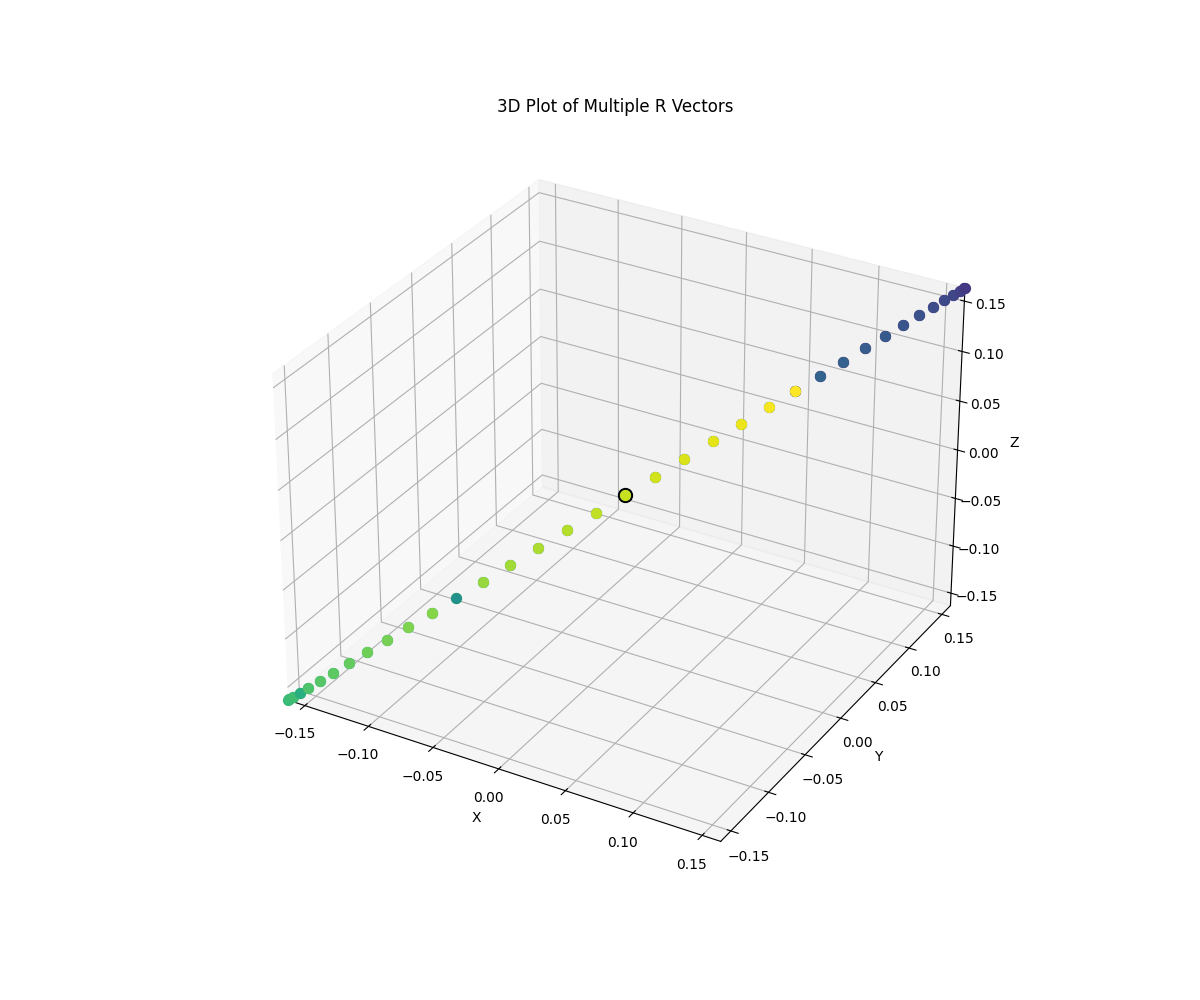
\includegraphics[width=0.8\textwidth]{figures/circle_3d.png}
    \caption{Example of endpoints-only visualization (orthogonal vector circle)}
    \label{fig:vis_endpoints_only}
\end{figure}

\subsection{Multiple Vector Visualization}

The system supports visualizing multiple vectors in a single plot, with the following features:

\begin{itemize}
    \item Multiple vectors can be generated by specifying ranges for the distance and angle parameters.
    \item Each vector is assigned a color from a colormap for easy identification.
    \item The plot includes a legend identifying each vector by its parameters.
    \item The endpoints-only option can be used to visualize the pattern formed by the endpoints of multiple vectors.
\end{itemize}

This capability is particularly useful for exploring the effects of varying parameters on the resulting vectors and for generating complex patterns such as circles and spheres.

\subsection{Circle Examples Visualization}

The system includes example scripts demonstrating different approaches to generating and visualizing circle and sphere-like patterns:

\begin{itemize}
    \item \texttt{example\_circle.py}: Generates points using orthogonal vector formulas, creating a sphere-like pattern.
    \item \texttt{example\_circle\_xy.py}: Creates a traditional circle in the XY plane.
    \item \texttt{example\_orthogonal\_circle.py}: Similar to the first example but with improved visualization.
\end{itemize}

These examples generate points at regular angular intervals and plot only the endpoints of the vectors, providing a clear visualization of the resulting patterns.

\begin{figure}[H]
    \centering
    \begin{minipage}{0.48\textwidth}
        \centering
        \includegraphics[width=\textwidth]{figures/circle_xy.png}
        \caption{XY projection of orthogonal vector circle}
        \label{fig:vis_circle_xy}
    \end{minipage}\hfill
    \begin{minipage}{0.48\textwidth}
        \centering
        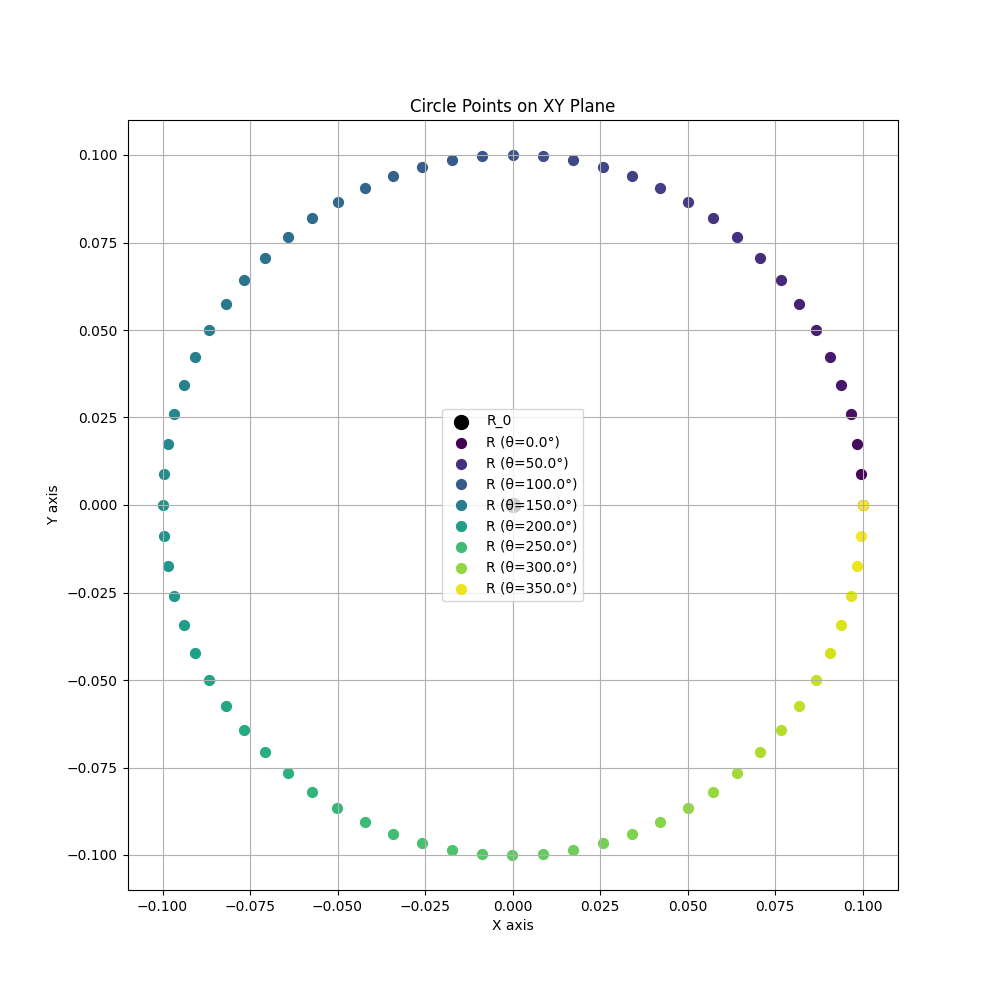
\includegraphics[width=\textwidth]{figures/xy_circle.png}
        \caption{Traditional circle in XY plane}
        \label{fig:vis_xy_circle}
    \end{minipage}
\end{figure}

\begin{figure}[H]
    \centering
    \includegraphics[width=0.8\textwidth]{figures/3d_xy_circle.png}
    \caption{3D visualization of traditional XY circle}
    \label{fig:vis_3d_xy_circle}
\end{figure}

\subsection{Enhanced Axis Representation}

The visualization system includes enhanced axis representation features for better spatial understanding:

\begin{itemize}
    \item \textbf{Color-coded Axes}: The X, Y, and Z axes are color-coded (X: red, Y: green, Z: blue) for easy identification.
    \item \textbf{Coordinate Labels}: Integer coordinate values are displayed along each axis, color-matched to the axis color.
    \item \textbf{Tick Marks}: Small tick marks are added along each axis for better spatial reference.
    \item \textbf{Axis Scaling}: The axis limits are dynamically adjusted based on the actual data points, with a small buffer for better visibility.
    \item \textbf{Equal Aspect Ratio}: The 3D plots maintain an equal aspect ratio for accurate spatial representation.
\end{itemize}

These enhancements significantly improve the visual representation of the orthogonal vectors, making it easier to understand their spatial relationships and properties.

\subsection{Implementation Details}

The visualization functions use Matplotlib to create the plots. The 3D visualization uses Matplotlib's \texttt{Axes3D} class, while the 2D visualizations use regular Matplotlib axes.

The vectors are plotted using Matplotlib's \texttt{quiver} function, which creates arrows from a starting point to an ending point. The origin point is plotted using Matplotlib's \texttt{scatter} function.

The colors of the vectors are assigned using Matplotlib's default color cycle or a specified colormap for multiple vectors, ensuring that each vector has a different color.

The axis lines are plotted using Matplotlib's \texttt{plot} function with specified colors and alpha values. Coordinate labels and tick marks are added using Matplotlib's \texttt{text} and \texttt{plot} functions.

The legends are created using Matplotlib's \texttt{legend} function, with labels for each vector.

The plots are saved using Matplotlib's \texttt{savefig} function, which supports various file formats, including PNG, JPEG, and PDF.

\subsection{Visualization in the Command-line Interface}

The command-line interface provides options for controlling the visualization, including:

\begin{itemize}
    \item \texttt{--plot-type}: Specifies the type of plot, either "3d" or "2d".
    \item \texttt{--title}: Specifies the title of the plot.
    \item \texttt{--no-show}: Prevents the plot from being displayed interactively.
    \item \texttt{--save-path}: Specifies the path to save the plot.
\end{itemize}

These options allow users to customize the visualization without modifying the code.

\newpage
\section{Configuration}

The Generalized Orthogonal Vectors Generator and Visualizer package provides a flexible configuration system that allows users to customize all aspects of vector generation and visualization. This section describes the configuration system and its features.

\subsection{VectorConfig Class}

The configuration system is implemented through the \texttt{VectorConfig} class, which provides a unified way to configure all aspects of vector generation and visualization. The class has the following attributes:

\begin{itemize}
    \item \texttt{origin}: The origin point for vector generation (default: [0, 0, 0]).
    \item \texttt{d}: The distance parameter for vector generation (default: 1.0).
    \item \texttt{theta}: The angle parameter for vector generation (default: $\pi/4$).
    \item \texttt{plot\_type}: The type of plot, either "3d" or "2d" (default: "3d").
    \item \texttt{title}: The title of the plot (default: None, which uses a default title based on the plot type).
    \item \texttt{show\_plot}: Whether to show the plot interactively (default: True).
    \item \texttt{save\_path}: The path to save the plot (default: None, which doesn't save the plot).
    \item \texttt{enhanced\_visualization}: Whether to use enhanced visualization features (default: True).
    \item \texttt{axis\_colors}: Custom colors for the X, Y, and Z axes (default: ['r', 'g', 'b']).
    \item \texttt{show\_coordinate\_labels}: Whether to show coordinate labels on the axes (default: True).
    \item \texttt{equal\_aspect\_ratio}: Whether to maintain an equal aspect ratio for 3D plots (default: True).
\end{itemize}

The class provides methods for initializing the configuration, saving it to a file, and loading it from a file.

\subsection{Initializing a Configuration}

A configuration can be initialized with default values or with custom values:

\begin{lstlisting}[language=Python]
# Initialize with default values
config = VectorConfig()

# Initialize with custom values
config = VectorConfig(
    origin=[1, 1, 1],
    d=2.0,
    theta=math.pi / 3,
    plot_type="2d",
    title="Vector Configuration",
    show_plot=False,
    save_path="custom.png",
    enhanced_visualization=True,
    axis_colors=['red', 'green', 'blue'],
    show_coordinate_labels=True,
    equal_aspect_ratio=True
)
\end{lstlisting}

\subsection{Using a Configuration}

A configuration can be used to generate and visualize orthogonal vectors:

\begin{lstlisting}[language=Python]
# Generate orthogonal vectors using the configuration
vectors = create_orthogonal_vectors(
    origin=config.origin,
    d=config.d,
    theta=config.theta
)

# Plot the vectors using the configuration
plot_vectors(
    vectors,
    origin=config.origin,
    plot_type=config.plot_type,
    title=config.title,
    show_plot=config.show_plot,
    save_path=config.save_path
)
\end{lstlisting}

\subsection{Saving a Configuration to a File}

A configuration can be saved to a JSON file for later use:

\begin{lstlisting}[language=Python]
# Save the configuration to a file
config.save_to_file("config.json")
\end{lstlisting}

The saved file will contain all the configuration parameters in JSON format:

\begin{lstlisting}[language=JSON]
{
    "origin": [1, 1, 1],
    "d": 2.0,
    "theta": 1.0471975511965976,
    "plot_type": "2d",
    "title": "Custom Configuration",
    "show_plot": false,
    "save_path": "custom.png"
}
\end{lstlisting}

\subsection{Loading a Configuration from a File}

A configuration can be loaded from a JSON file:

\begin{lstlisting}[language=Python]
# Load the configuration from a file
config = VectorConfig.load_from_file("config.json")
\end{lstlisting}

This creates a new \texttt{VectorConfig} object with the parameters specified in the file.

\subsection{Configuration in the Command-line Interface}

The command-line interface provides options for configuring vector generation and visualization:

\begin{itemize}
    \item \texttt{--origin}: Specifies the origin point as three space-separated values.
    \item \texttt{--d}: Specifies the distance parameter.
    \item \texttt{--theta}: Specifies the angle parameter in radians.
    \item \texttt{--plot-type}: Specifies the type of plot, either "3d" or "2d".
    \item \texttt{--title}: Specifies the title of the plot.
    \item \texttt{--no-show}: Prevents the plot from being displayed interactively.
    \item \texttt{--save-path}: Specifies the path to save the plot.
    \item \texttt{--config}: Specifies a configuration file to load.
    \item \texttt{--save-config}: Specifies a file to save the configuration to.
    \item \texttt{--no-enhanced-visualization}: Disables enhanced visualization features.
    \item \texttt{--axis-colors}: Specifies custom colors for the X, Y, and Z axes as three space-separated values.
    \item \texttt{--no-coordinate-labels}: Disables coordinate labels on the axes.
    \item \texttt{--no-equal-aspect-ratio}: Disables equal aspect ratio for 3D plots.
\end{itemize}

These options allow users to customize the configuration without modifying the code.

\subsection{Configuration File Format}

The configuration file is a JSON file with the following structure:

\begin{lstlisting}[language=JSON]
{
    "origin": [x, y, z],
    "d": float,
    "theta": float,
    "plot_type": "3d" or "2d",
    "title": string or null,
    "show_plot": boolean,
    "save_path": string or null,
    "enhanced_visualization": boolean,
    "axis_colors": ["r", "g", "b"],
    "show_coordinate_labels": boolean,
    "equal_aspect_ratio": boolean
}
\end{lstlisting}

All fields are optional and will use default values if not specified.

\subsection{Default Configuration}

The default configuration is as follows:

\begin{itemize}
    \item \texttt{origin}: [0, 0, 0]
    \item \texttt{d}: 1.0
    \item \texttt{theta}: $\pi/4$ (approximately 0.7853981633974483)
    \item \texttt{plot\_type}: "3d"
    \item \texttt{title}: None (uses a default title based on the plot type)
    \item \texttt{show\_plot}: True
    \item \texttt{save\_path}: None (doesn't save the plot)
    \item \texttt{enhanced\_visualization}: True
    \item \texttt{axis\_colors}: ['r', 'g', 'b']
    \item \texttt{show\_coordinate\_labels}: True
    \item \texttt{equal\_aspect\_ratio}: True
\end{itemize}

This configuration generates three orthogonal vectors from the origin [0, 0, 0] with a distance parameter of 1.0 and an angle parameter of $\pi/4$, and visualizes them in 3D.

\newpage
\section{Command-line Interface}

The Generalized Arrowhead Framework provides a comprehensive command-line interface that allows users to generate and visualize vectors orthogonal to the x=y=z line, as well as generate and analyze arrowhead matrices. This section describes the command-line interface and its features.

\subsection{Basic Usage}

The command-line interface can be accessed by running the \texttt{main.py} module with the appropriate subcommand:

\begin{lstlisting}[language=bash]
# For vector generation and visualization
python generalized/main.py vector

# For arrowhead matrix generation and analysis
python generalized/main.py arrowhead

# For detailed help information
python generalized/main.py help
\end{lstlisting}

The \texttt{vector} subcommand generates and visualizes a single vector with default parameters (origin at [0, 0, 0], d=1.0, theta=pi/4).

The \texttt{arrowhead} subcommand generates and analyzes arrowhead matrices with default parameters (4x4 matrix, 72 theta steps).

\subsection{Command-line Options}

The command-line interface provides extensive options for both vector generation and arrowhead matrix analysis. The options are organized by subcommand.

\subsubsection{Vector Generation Options}

The following options are available for the \texttt{vector} subcommand:

\begin{itemize}
    \item \texttt{-R X Y Z}, \texttt{--origin X Y Z}: Sets the origin vector R\_0 coordinates. Default: 0 0 0.
    \item \texttt{-d VALUE}, \texttt{--distance VALUE}: Sets the distance parameter. Default: 1.0.
    \item \texttt{--d-range START STEPS END}: Generates multiple vectors with distance values from START to END with STEPS steps.
    \item \texttt{-a VALUE}, \texttt{--angle VALUE}, \texttt{--theta VALUE}: Sets the angle parameter in radians. Default: 0.7853981633974483 (pi/4).
    \item \texttt{--theta-range START STEPS END}: Generates multiple vectors with angle values from START to END with STEPS steps.
    \item \texttt{--perfect}: Uses the perfect orthogonal circle method for vector generation.
    \item \texttt{--plot-type TYPE}: Specifies the type of plot, either "3d" or "2d". Default: "3d".
    \item \texttt{--title TITLE}: Specifies the title of the plot.
    \item \texttt{--no-show}: Prevents the plot from being displayed interactively.
    \item \texttt{--save-path PATH}: Specifies the path to save the plot.
    \item \texttt{--no-enhanced-visualization}: Disables enhanced visualization features.
    \item \texttt{--axis-colors X Y Z}: Sets custom colors for the X, Y, and Z axes. Default: 'r g b'.
    \item \texttt{--no-coordinate-labels}: Disables coordinate labels on the axes.
    \item \texttt{--no-equal-aspect-ratio}: Disables equal aspect ratio for 3D plots.
    \item \texttt{--buffer-factor VALUE}: Sets the buffer factor for axis limits. Default: 0.2.
    \item \texttt{--no-r0-plane}: Does not show the R\_0 plane projection.
    \item \texttt{--no-legend}: Does not show the legend.
    \item \texttt{--no-grid}: Does not show the grid.
    \item \texttt{--endpoints true/false}: Only plot the endpoints of vectors, not the arrows. Default: false.
    \item \texttt{--save-plots}: Save plots to files instead of displaying them.
    \item \texttt{--output-dir DIR}: Directory to save plots to. Default: 'plots'.
    \item \texttt{--config FILE}: Load configuration from a JSON file.
    \item \texttt{--save-config FILE}: Save current configuration to a JSON file.
\end{itemize}

\subsubsection{Arrowhead Matrix Options}

The following options are available for the \texttt{arrowhead} subcommand:

\begin{itemize}
    \item \texttt{--r0 X Y Z}: Origin vector coordinates. Default: 0 0 0.
    \item \texttt{--d VALUE}: Distance parameter. Default: 0.5.
    \item \texttt{--theta-start VALUE}: Starting theta value in radians. Default: 0.
    \item \texttt{--theta-end VALUE}: Ending theta value in radians. Default: $2\pi$.
    \item \texttt{--theta-steps VALUE}: Number of theta values to generate matrices for. Default: 72.
    \item \texttt{--coupling VALUE}: Coupling constant for off-diagonal elements. Default: 0.1.
    \item \texttt{--omega VALUE}: Angular frequency for the energy term $\hbar\omega$. Default: 1.0.
    \item \texttt{--size VALUE}: Size of the matrix to generate. Default: 4.
    \item \texttt{--perfect}: Use perfect circle generation method. Default: True.
    \item \texttt{--output-dir DIR}: Directory to save results. Default: './results'.
    \item \texttt{--load-only}: Only load existing results and create plots.
    \item \texttt{--plot-only}: Only create plots from existing results.
\end{itemize}



\subsection{Examples}

\subsubsection{Vector Generation Examples}

\paragraph{Generating a Single Vector}

\begin{lstlisting}[language=bash]
python generalized/main.py vector -R 1 1 1 -d 2.0 -a 1.047
\end{lstlisting}

This command generates and visualizes a single vector with custom parameters (origin at [1, 1, 1], d=2.0, theta=pi/3).

\paragraph{Generating Multiple Vectors with Distance Range}

\begin{lstlisting}[language=bash]
python generalized/main.py vector -R 0 0 0 --d-range 1 5 3 -a 0.7854
\end{lstlisting}

This command generates and visualizes multiple vectors with varying distance values (from 1 to 3 in 5 steps) and fixed angle (pi/4).

\paragraph{Generating Multiple Vectors with Angle Range}

\begin{lstlisting}[language=bash]
python generalized/main.py vector -R 0 0 0 -d 1.5 --theta-range 0 10 3.14159
\end{lstlisting}

This command generates and visualizes multiple vectors with fixed distance (1.5) and varying angle values (from 0 to pi in 10 steps).

\paragraph{Using 2D Plot Type}

\begin{lstlisting}[language=bash]
python generalized/main.py vector --plot-type 2d --title "2D Projection of Orthogonal Vector"
\end{lstlisting}

This command generates a vector with default parameters and displays it using a 2D plot with a custom title.

\paragraph{Customizing Visualization}

\begin{lstlisting}[language=bash]
python generalized/main.py vector --axis-colors blue green red --no-coordinate-labels
\end{lstlisting}

This command generates a vector with default parameters and customizes the visualization with custom axis colors and no coordinate labels.

\paragraph{Saving to a Specific Path}

\begin{lstlisting}[language=bash]
python generalized/main.py vector --no-show --save-path "./figures/orthogonal_vector.png"
\end{lstlisting}

\subsubsection{Arrowhead Matrix Examples}

\paragraph{Generating Matrices with Default Parameters}

\begin{lstlisting}[language=bash]
python generalized/main.py arrowhead
\end{lstlisting}

This command generates and analyzes arrowhead matrices with default parameters (4x4 matrix, 72 theta steps).

\paragraph{Generating Matrices with Custom Parameters}

\begin{lstlisting}[language=bash]
python generalized/main.py arrowhead --r0 1 1 1 --d 0.8 --theta-steps 36 --size 6
\end{lstlisting}

This command generates and analyzes 6x6 arrowhead matrices with custom parameters (origin at [1, 1, 1], d=0.8, 36 theta steps).

\paragraph{Using Perfect Circle Generation}

\begin{lstlisting}[language=bash]
python generalized/main.py arrowhead --perfect --theta-steps 12
\end{lstlisting}

This command generates and analyzes arrowhead matrices using the perfect circle generation method with 12 theta steps.

\paragraph{Only Creating Plots from Existing Results}

\begin{lstlisting}[language=bash]
python generalized/main.py arrowhead --plot-only --output-dir my_results
\end{lstlisting}

This command only creates plots from existing results in the specified directory.

\paragraph{Loading Existing Results and Creating Plots}

\begin{lstlisting}[language=bash]
python generalized/main.py arrowhead --load-only --output-dir my_results
\end{lstlisting}

This command loads existing results from the specified directory and creates plots.

\subsubsection{Endpoints-only Plotting}

\begin{lstlisting}[language=bash]
python generalized/main.py --endpoints true
\end{lstlisting}

This command generates a vector with default parameters and plots only the endpoints, not the arrows.

\subsubsection{Saving Plots}

\begin{lstlisting}[language=bash]
python generalized/main.py --save-plots --output-dir my_plots
\end{lstlisting}

This command generates a vector with default parameters and saves the plots to the 'my\_plots' directory.

\subsubsection{Using a Configuration File}

\begin{lstlisting}[language=bash]
python generalized/main.py --config my_config.json
\end{lstlisting}

This command loads a configuration from a file and uses it to generate and visualize vectors.

\subsubsection{Saving a Configuration File}

\begin{lstlisting}[language=bash]
python generalized/main.py -R 1 1 1 -d 2.0 -a 1.047 --save-config my_config.json
\end{lstlisting}

This command generates and visualizes a vector with custom parameters and saves the configuration to a file.

\subsection{Configuration File Format}

The configuration file is a JSON file with the following structure:

\begin{lstlisting}[language=json]
{
    "origin": [x, y, z],
    "d": float,
    "theta": float,
    "plot_type": "3d" or "2d",
    "title": string or null,
    "show_plot": boolean,
    "save_path": string or null,
    "enhanced_visualization": boolean,
    "axis_colors": ["r", "g", "b"],
    "show_coordinate_labels": boolean,
    "equal_aspect_ratio": boolean,
    "buffer_factor": float,
    "show_r0_plane": boolean,
    "show_legend": boolean,
    "show_grid": boolean,
    "perfect": boolean
}
\end{lstlisting}

All fields are optional and will use default values if not specified. The default configuration is as follows:

\begin{itemize}
    \item \texttt{origin}: [0, 0, 0]
    \item \texttt{d}: 1.0
    \item \texttt{theta}: $\pi/4$ (approximately 0.7853981633974483)
    \item \texttt{plot\_type}: "3d"
    \item \texttt{title}: null (uses a default title based on the plot type)
    \item \texttt{show\_plot}: true
    \item \texttt{save\_path}: null (doesn't save the plot)
    \item \texttt{enhanced\_visualization}: true
    \item \texttt{axis\_colors}: ["r", "g", "b"]
    \item \texttt{show\_coordinate\_labels}: true
    \item \texttt{equal\_aspect\_ratio}: true
    \item \texttt{buffer\_factor}: 0.2
    \item \texttt{show\_r0\_plane}: true
    \item \texttt{show\_legend}: true
    \item \texttt{show\_grid}: true
    \item \texttt{perfect}: false
\end{itemize}

\subsection{Circle Examples}

The system includes several example scripts for generating and visualizing circle and sphere-like patterns:

\begin{lstlisting}[language=bash]
# Generate a sphere-like pattern using vectors orthogonal to the x=y=z line
python generalized/example_circle.py

# Generate a traditional circle in the XY plane
python generalized/example_circle_xy.py

# Generate a sphere-like pattern with improved visualization
# using vectors orthogonal to the x=y=z line
python generalized/example_orthogonal_circle.py

# Generate a perfect circle in the plane orthogonal to the x=y=z line
# with enhanced visualization features
python perfect_orthogonal_circle.py

# Generate multiple perfect circles at different distances
# with enhanced visualization features
python perfect_circle_distance_range.py
\end{lstlisting}

These examples generate 73 points (from 0\textdegree\ to 360\textdegree\ in 5\textdegree\ increments) and plot only the endpoints of the vectors, providing a clear visualization of the patterns formed. The orthogonality to the x=y=z line is ensured by using the basis vectors [1, -1/2, -1/2] and [0, -1/2, 1/2] in the vector generation process.

\subsection{Implementation Details}

The command-line interface is implemented in the \texttt{main.py} module using the \texttt{argparse} module from the Python standard library. The module defines a \texttt{main} function that parses command-line arguments, creates a configuration, generates vectors, and visualizes them.

The command-line interface follows these steps:

\begin{enumerate}
    \item Parse command-line arguments using \texttt{argparse}.
    \item If a configuration file is specified, load the configuration from the file.
    \item Override the configuration with any command-line options that are specified.
    \item Generate a vector using the scalar-based formula and the configuration.
    \item If requested, analyze the properties of the generated vector and print the result.
    \item If verbose output is enabled, print vector coordinates and properties.
    \item Visualize the vectors using the configuration.
    \item If requested, save the configuration to a file.
\end{enumerate}

\subsection{Error Handling}

The command-line interface includes error handling for various scenarios, including:

\begin{itemize}
    \item Invalid command-line arguments (e.g., non-numeric values for numeric options).
    \item Invalid configuration file (e.g., file not found, invalid JSON).
    \item Invalid configuration parameters (e.g., negative distance parameter).
\end{itemize}

When an error occurs, the command-line interface prints an error message and exits with a non-zero exit code.

\subsection{Help Message}

The command-line interface provides a help message that can be displayed using the \texttt{--help} option:

\begin{lstlisting}[language=bash]
python -m generalized.main --help
\end{lstlisting}

The help message includes a description of the program, a list of all available options, and examples of how to use the program.


\newpage
\section{Example Results}

This section presents example results for different configurations of the Orthogonal Vector Visualization System. It shows the generated vectors and their visualizations for various parameter values.

\subsection{Single Vector Generation}

The system generates a single R vector using scalar formulas. The default configuration uses the origin [0, 0, 0] with a distance parameter of 1.0 and an angle parameter of $\pi/4$.

\subsubsection{Scalar Formulation}

The R vector is calculated using the following scalar formula:

\begin{align}
\vec{R} = \vec{R}_0 + d \cdot \cos(\theta) \cdot \sqrt{\frac{2}{3}} + d \cdot \frac{\cos(\theta)/\sqrt{3} + \sin(\theta)}{\sqrt{2}} + d \cdot \frac{\sin(\theta) - \cos(\theta)/\sqrt{3}}{\sqrt{2}} - 2 \cdot \vec{R}_0
\end{align}

This formula combines three orthogonal components to produce a single resulting vector.

\subsubsection{3D Visualization}

\begin{figure}[H]
    \centering
    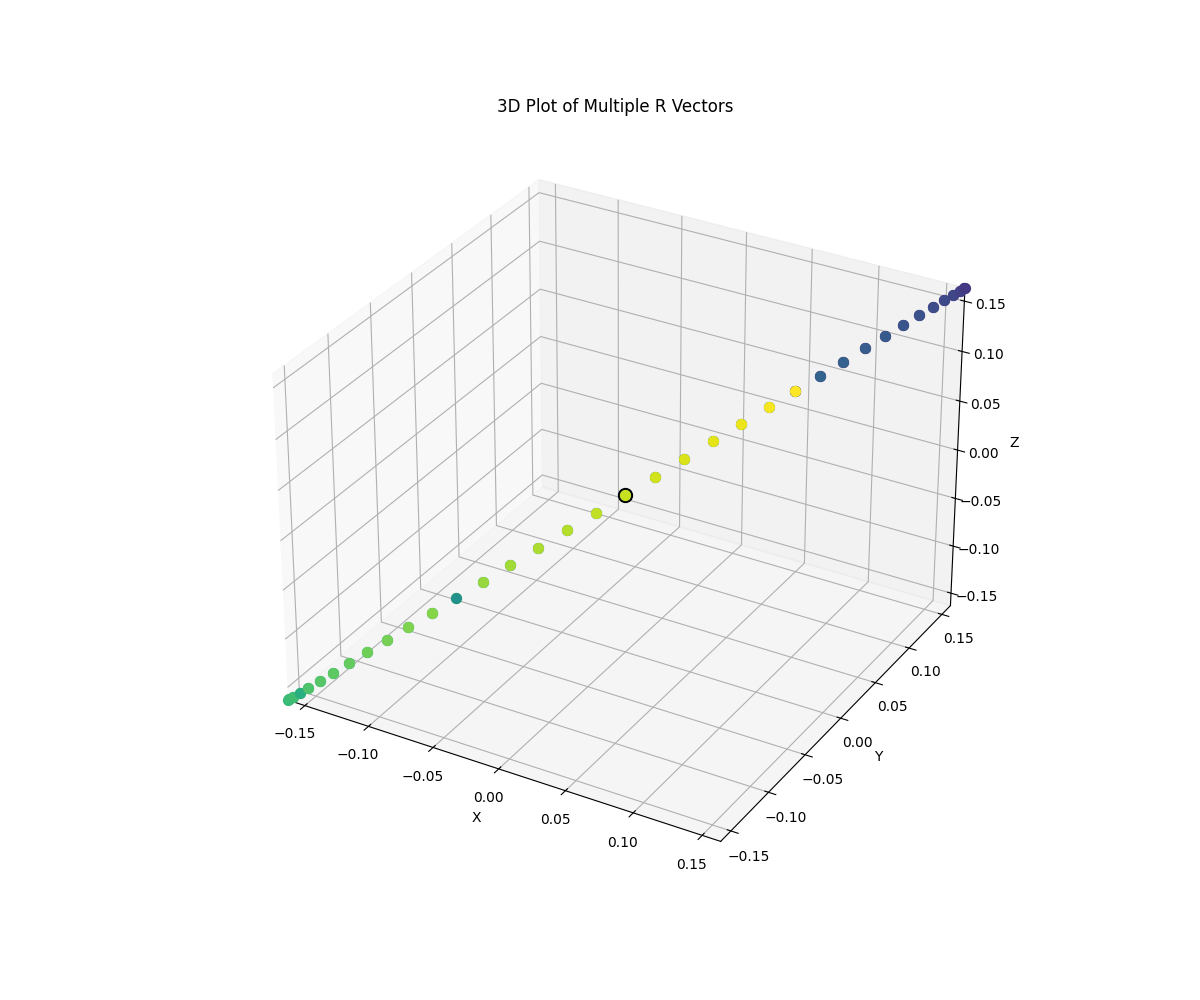
\includegraphics[width=0.8\textwidth]{figures/circle_3d.png}
    \caption{3D visualization of the orthogonal vector configuration}
    \label{fig:example_default_3d}
\end{figure}

\subsubsection{2D Projections}

\begin{figure}[H]
    \centering
    \includegraphics[width=0.45\textwidth]{figures/circle_xy.png}
    \includegraphics[width=0.45\textwidth]{figures/circle_xz.png}
    \includegraphics[width=0.45\textwidth]{figures/circle_yz.png}
    \includegraphics[width=0.45\textwidth]{figures/circle_r0.png}
    \caption{2D projections of the orthogonal vector configuration}
    \label{fig:example_default_2d}
\end{figure}

\subsection{Multiple Vector Generation}

The system supports generating multiple vectors by specifying ranges for the distance and angle parameters. This is particularly useful for exploring the effects of varying parameters on the resulting vectors and for generating complex patterns.

\subsubsection{Distance Range Example}

This example generates multiple vectors with varying distance values (from 1 to 3 in 5 steps) and a fixed angle ($\pi/4$):

\begin{lstlisting}[language=bash]
python generalized/main.py -R 0 0 0 --d-range 1 5 3 -a 0.7854
\end{lstlisting}

\subsubsection{Angle Range Example}

This example generates multiple vectors with a fixed distance (1.5) and varying angle values (from 0 to $\pi$ in 10 steps):

\begin{lstlisting}[language=bash]
python generalized/main.py -R 0 0 0 -d 1.5 --theta-range 0 10 3.14159
\end{lstlisting}

\subsection{Circle Examples}

The system includes three example scripts demonstrating different approaches to generating and visualizing circle and sphere-like patterns. Each example generates 73 points (from 0\textdegree\ to 360\textdegree\ in 5\textdegree\ increments) and plots only the endpoints of the vectors.

\subsubsection{Orthogonal Vector Circle}

The \texttt{example\_circle.py} script generates points using orthogonal vector formulas, creating a sphere-like pattern:

\begin{lstlisting}[language=bash]
python generalized/example_circle.py
\end{lstlisting}

\begin{figure}[H]
    \centering
    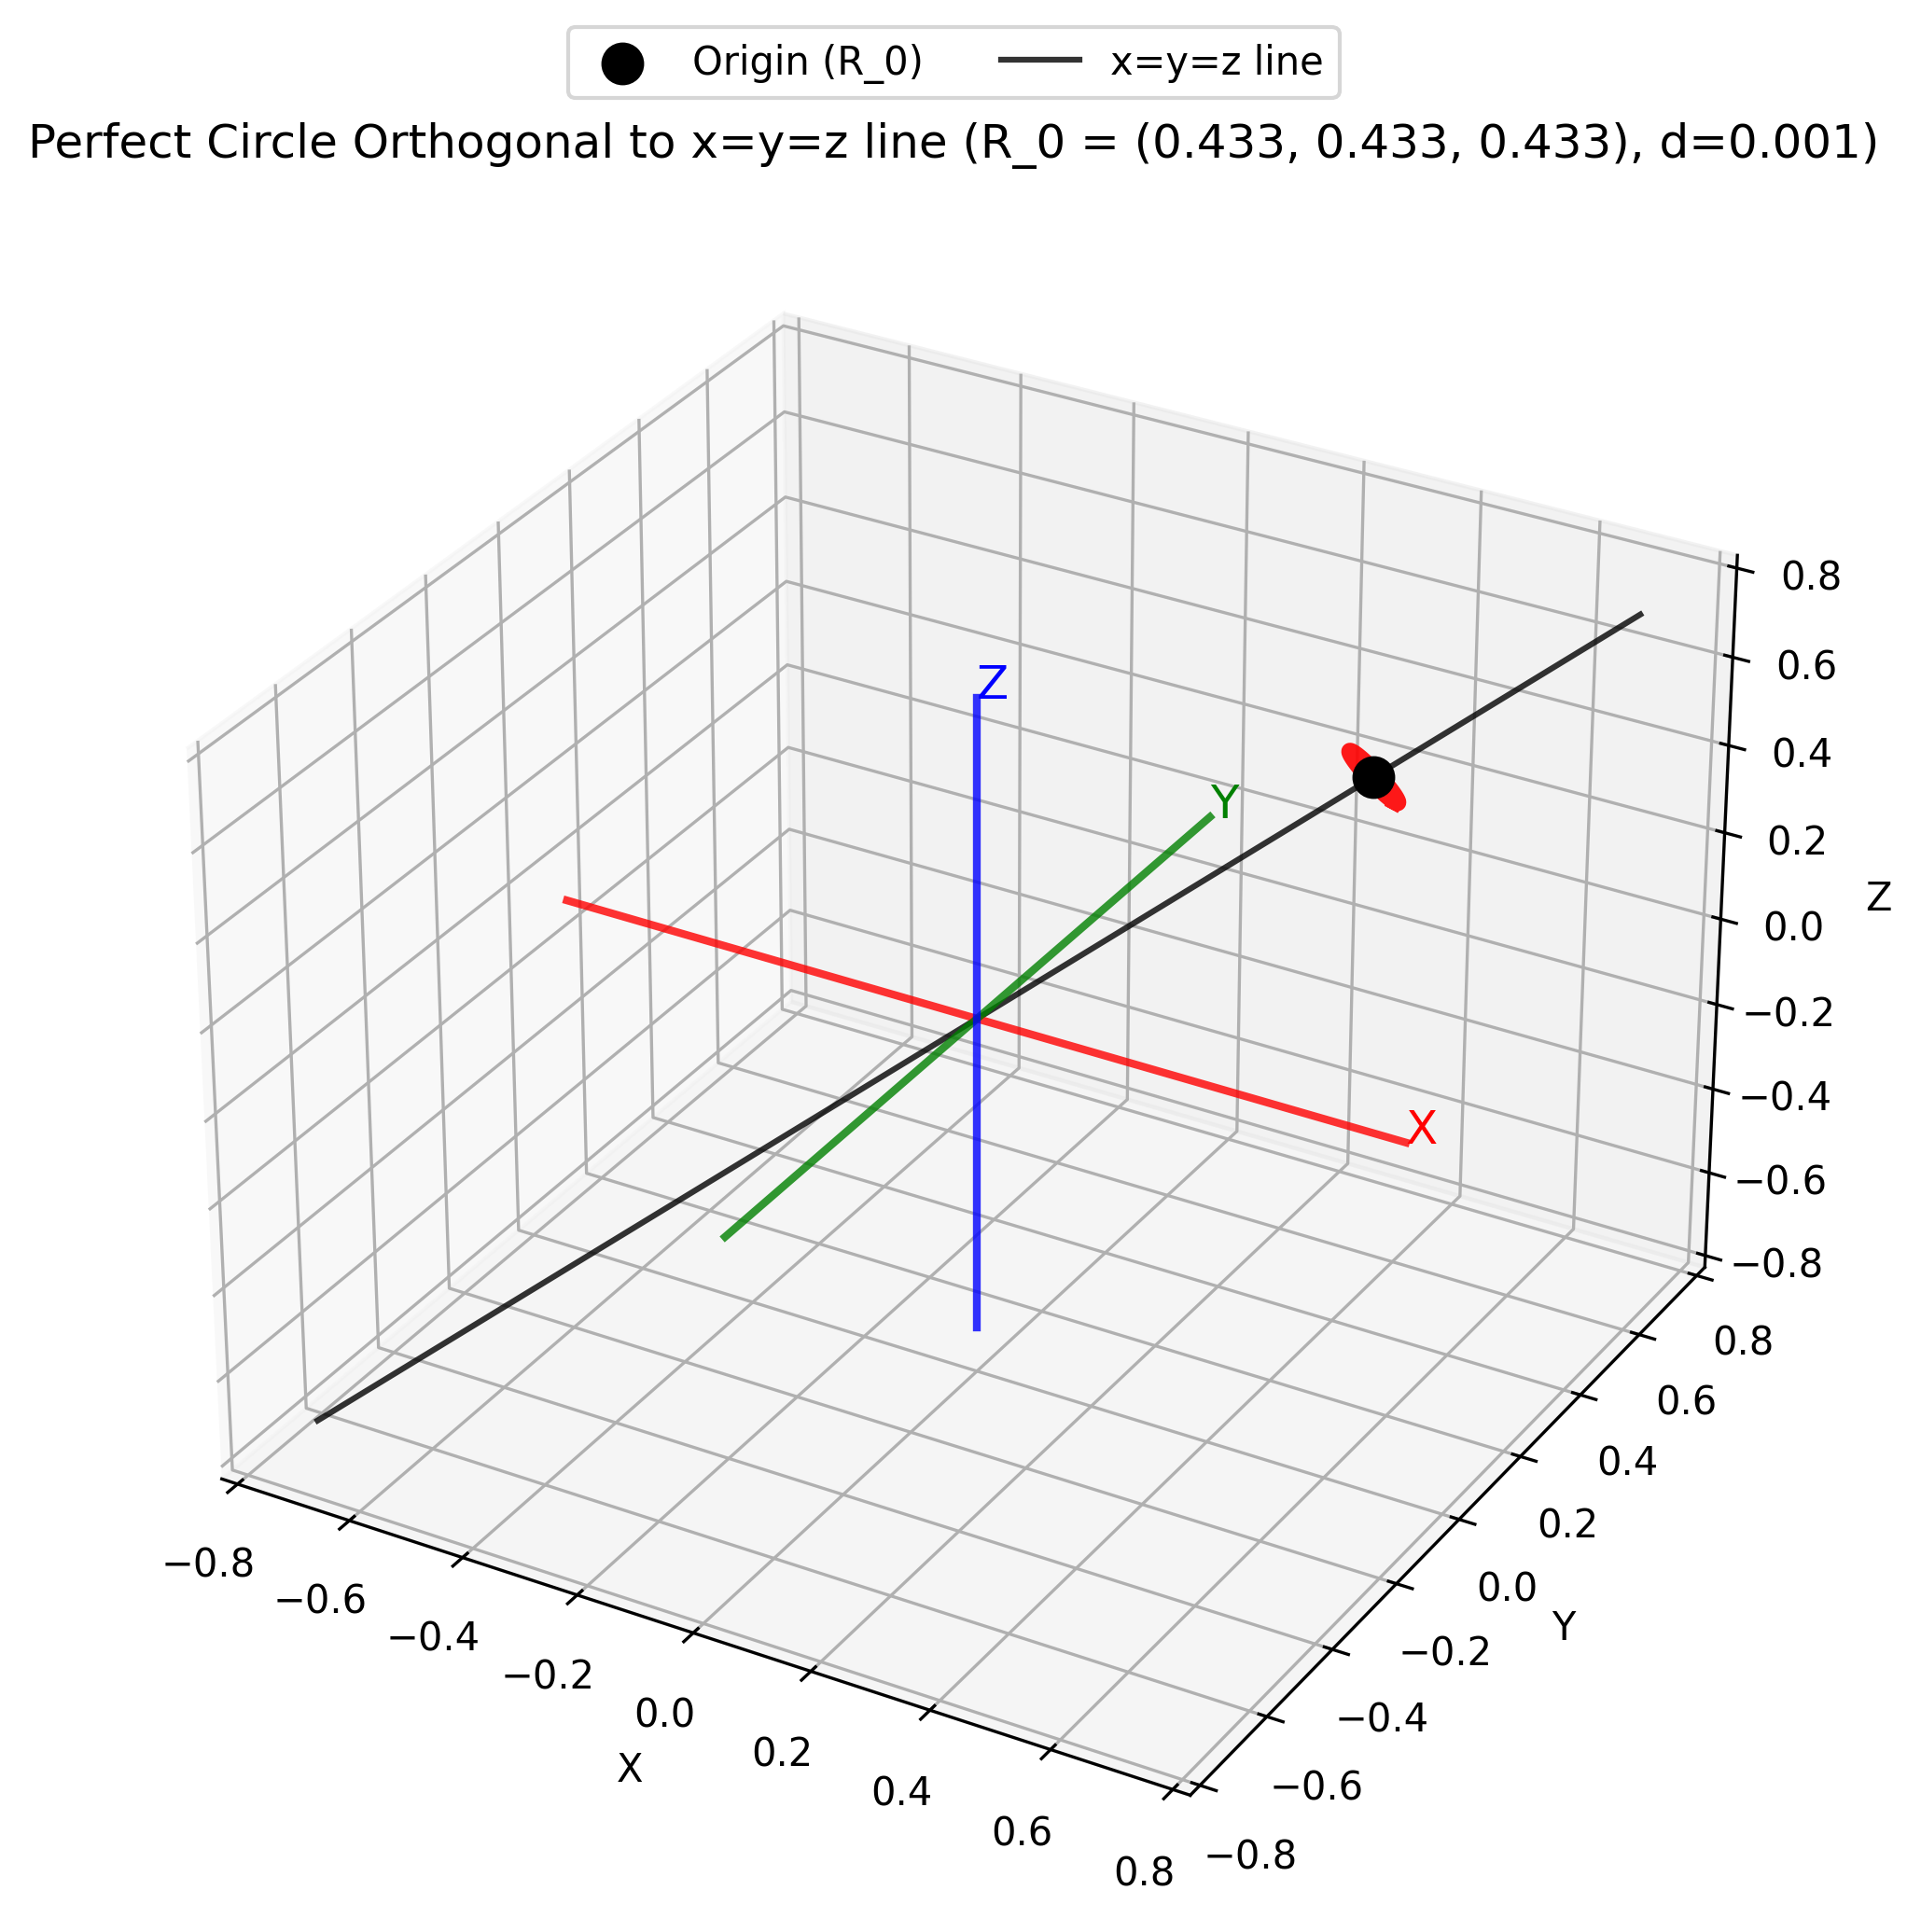
\includegraphics[width=0.8\textwidth]{../../../circle_plots/circle_3d.png}
    \caption{3D visualization of the orthogonal vector circle}
    \label{fig:example_circle_3d}
\end{figure}

\begin{figure}[H]
    \centering
    \begin{minipage}{0.48\textwidth}
        \centering
        \includegraphics[width=\textwidth]{../../../circle_plots/circle_xy.png}
        \caption{XY projection of the orthogonal vector circle}
        \label{fig:example_circle_xy}
    \end{minipage}\hfill
    \begin{minipage}{0.48\textwidth}
        \centering
        \includegraphics[width=\textwidth]{../../../circle_plots/circle_xz.png}
        \caption{XZ projection of the orthogonal vector circle}
        \label{fig:example_circle_xz}
    \end{minipage}
\end{figure}

\begin{figure}[H]
    \centering
    \begin{minipage}{0.48\textwidth}
        \centering
        \includegraphics[width=\textwidth]{../../../circle_plots/circle_yz.png}
        \caption{YZ projection of the orthogonal vector circle}
        \label{fig:example_circle_yz}
    \end{minipage}\hfill
    \begin{minipage}{0.48\textwidth}
        \centering
        \includegraphics[width=\textwidth]{../../../circle_plots/circle_r0.png}
        \caption{Origin plane projection of the orthogonal vector circle}
        \label{fig:example_circle_origin}
    \end{minipage}
\end{figure}

\subsubsection{Traditional XY Circle}

The \texttt{example\_circle\_xy.py} script creates a traditional circle in the XY plane:

\begin{lstlisting}[language=bash]
python generalized/example_circle_xy.py
\end{lstlisting}

\begin{figure}[H]
    \centering
    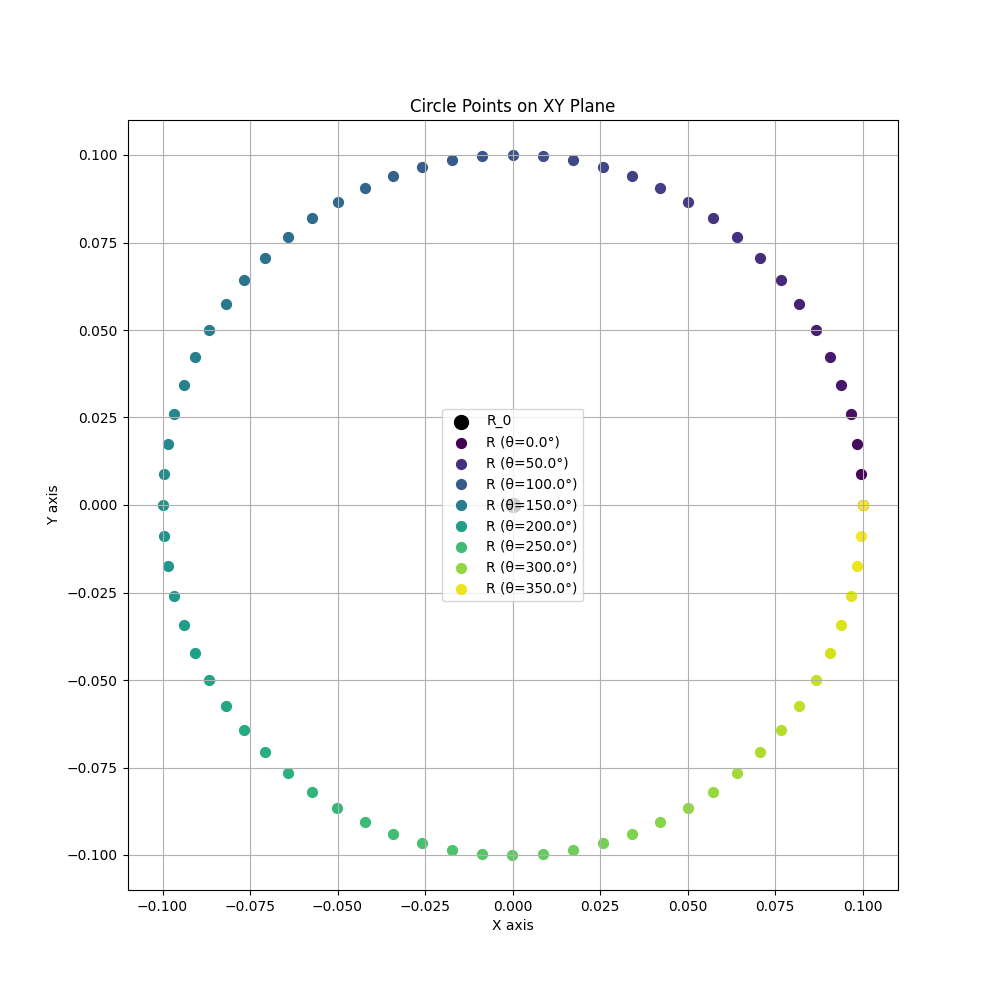
\includegraphics[width=0.8\textwidth]{figures/xy_circle.png}
    \caption{Traditional circle in the XY plane}
    \label{fig:example_xy_circle}
\end{figure}

\begin{figure}[H]
    \centering
    \includegraphics[width=0.8\textwidth]{../../../circle_plots/3d_xy_circle.png}
    \caption{3D visualization of the traditional XY circle}
    \label{fig:example_3d_xy_circle}
\end{figure}

\subsubsection{Improved Orthogonal Vector Circle}

The \texttt{example\_orthogonal\_circle.py} script is similar to the first example but with improved visualization:

\begin{lstlisting}[language=bash]
python generalized/example_orthogonal_circle.py
\end{lstlisting}

\begin{figure}[H]
    \centering
    \includegraphics[width=0.8\textwidth]{../../../circle_plots/orthogonal_3d.png}
    \caption{3D visualization of the improved orthogonal vector circle}
    \label{fig:example_orthogonal_3d}
\end{figure}

\begin{figure}[H]
    \centering
    \begin{minipage}{0.48\textwidth}
        \centering
        \includegraphics[width=\textwidth]{../../../circle_plots/orthogonal_xy.png}
        \caption{XY projection of the improved orthogonal vector circle}
        \label{fig:example_orthogonal_xy}
    \end{minipage}\hfill
    \begin{minipage}{0.48\textwidth}
        \centering
        \includegraphics[width=\textwidth]{../../../circle_plots/orthogonal_xz.png}
        \caption{XZ projection of the improved orthogonal vector circle}
        \label{fig:example_orthogonal_xz}
    \end{minipage}
\end{figure}

\begin{figure}[H]
    \centering
    \begin{minipage}{0.48\textwidth}
        \centering
        \includegraphics[width=\textwidth]{../../../circle_plots/orthogonal_yz.png}
        \caption{YZ projection of the improved orthogonal vector circle}
        \label{fig:example_orthogonal_yz}
    \end{minipage}\hfill
    \begin{minipage}{0.48\textwidth}
        \centering
        \includegraphics[width=\textwidth]{../../../circle_plots/orthogonal_r0.png}
        \caption{Origin plane projection of the improved orthogonal vector circle}
        \label{fig:example_orthogonal_origin}
    \end{minipage}
\end{figure}








\subsection{Perfect Orthogonal Circle Generation}

This section presents the implementation of a perfect circle generator in the plane orthogonal to the x=y=z line. This implementation ensures that all points on the circle are exactly at the specified distance from the origin and perfectly orthogonal to the (1,1,1) direction.

\subsubsection{Implementation Approach}

The perfect orthogonal circle is generated using normalized basis vectors that span the plane orthogonal to the (1,1,1) direction:

\begin{itemize}
    \item Basis vector 1: $[1, -1/2, -1/2]$ (normalized)
    \item Basis vector 2: $[0, -1/2, 1/2]$ (normalized)
\end{itemize}

Points on the circle are generated using the parametric circle equation with these basis vectors:

\begin{align}
\vec{p} = \vec{R}_0 + d \cdot (\cos(\theta) \cdot \vec{basis}_1 + \sin(\theta) \cdot \vec{basis}_2)
\end{align}

where $\vec{R}_0$ is the origin point, $d$ is the distance parameter, and $\theta$ ranges from 0 to $2\pi$.

\subsubsection{Verification Results}

The implementation was verified with the following parameters:
\begin{itemize}
    \item Origin vector (R\_0): [0, 0, 0]
    \item Distance parameter (d): 1.0
    \item Number of points: 73 (5-degree increments)
\end{itemize}

Verification results confirm perfect circle properties:
\begin{itemize}
    \item Mean distance from origin: exactly 1.0
    \item Standard deviation of distances: 8.01e-17 (effectively 0)
    \item Min/max distance ratio: 1.0000000000000004 (effectively 1.0)
    \item Maximum dot product with (1,1,1): 1.11e-16 (effectively 0)
    \item Average dot product with (1,1,1): 2.88e-17 (effectively 0)
\end{itemize}

\begin{figure}[H]
    \centering
    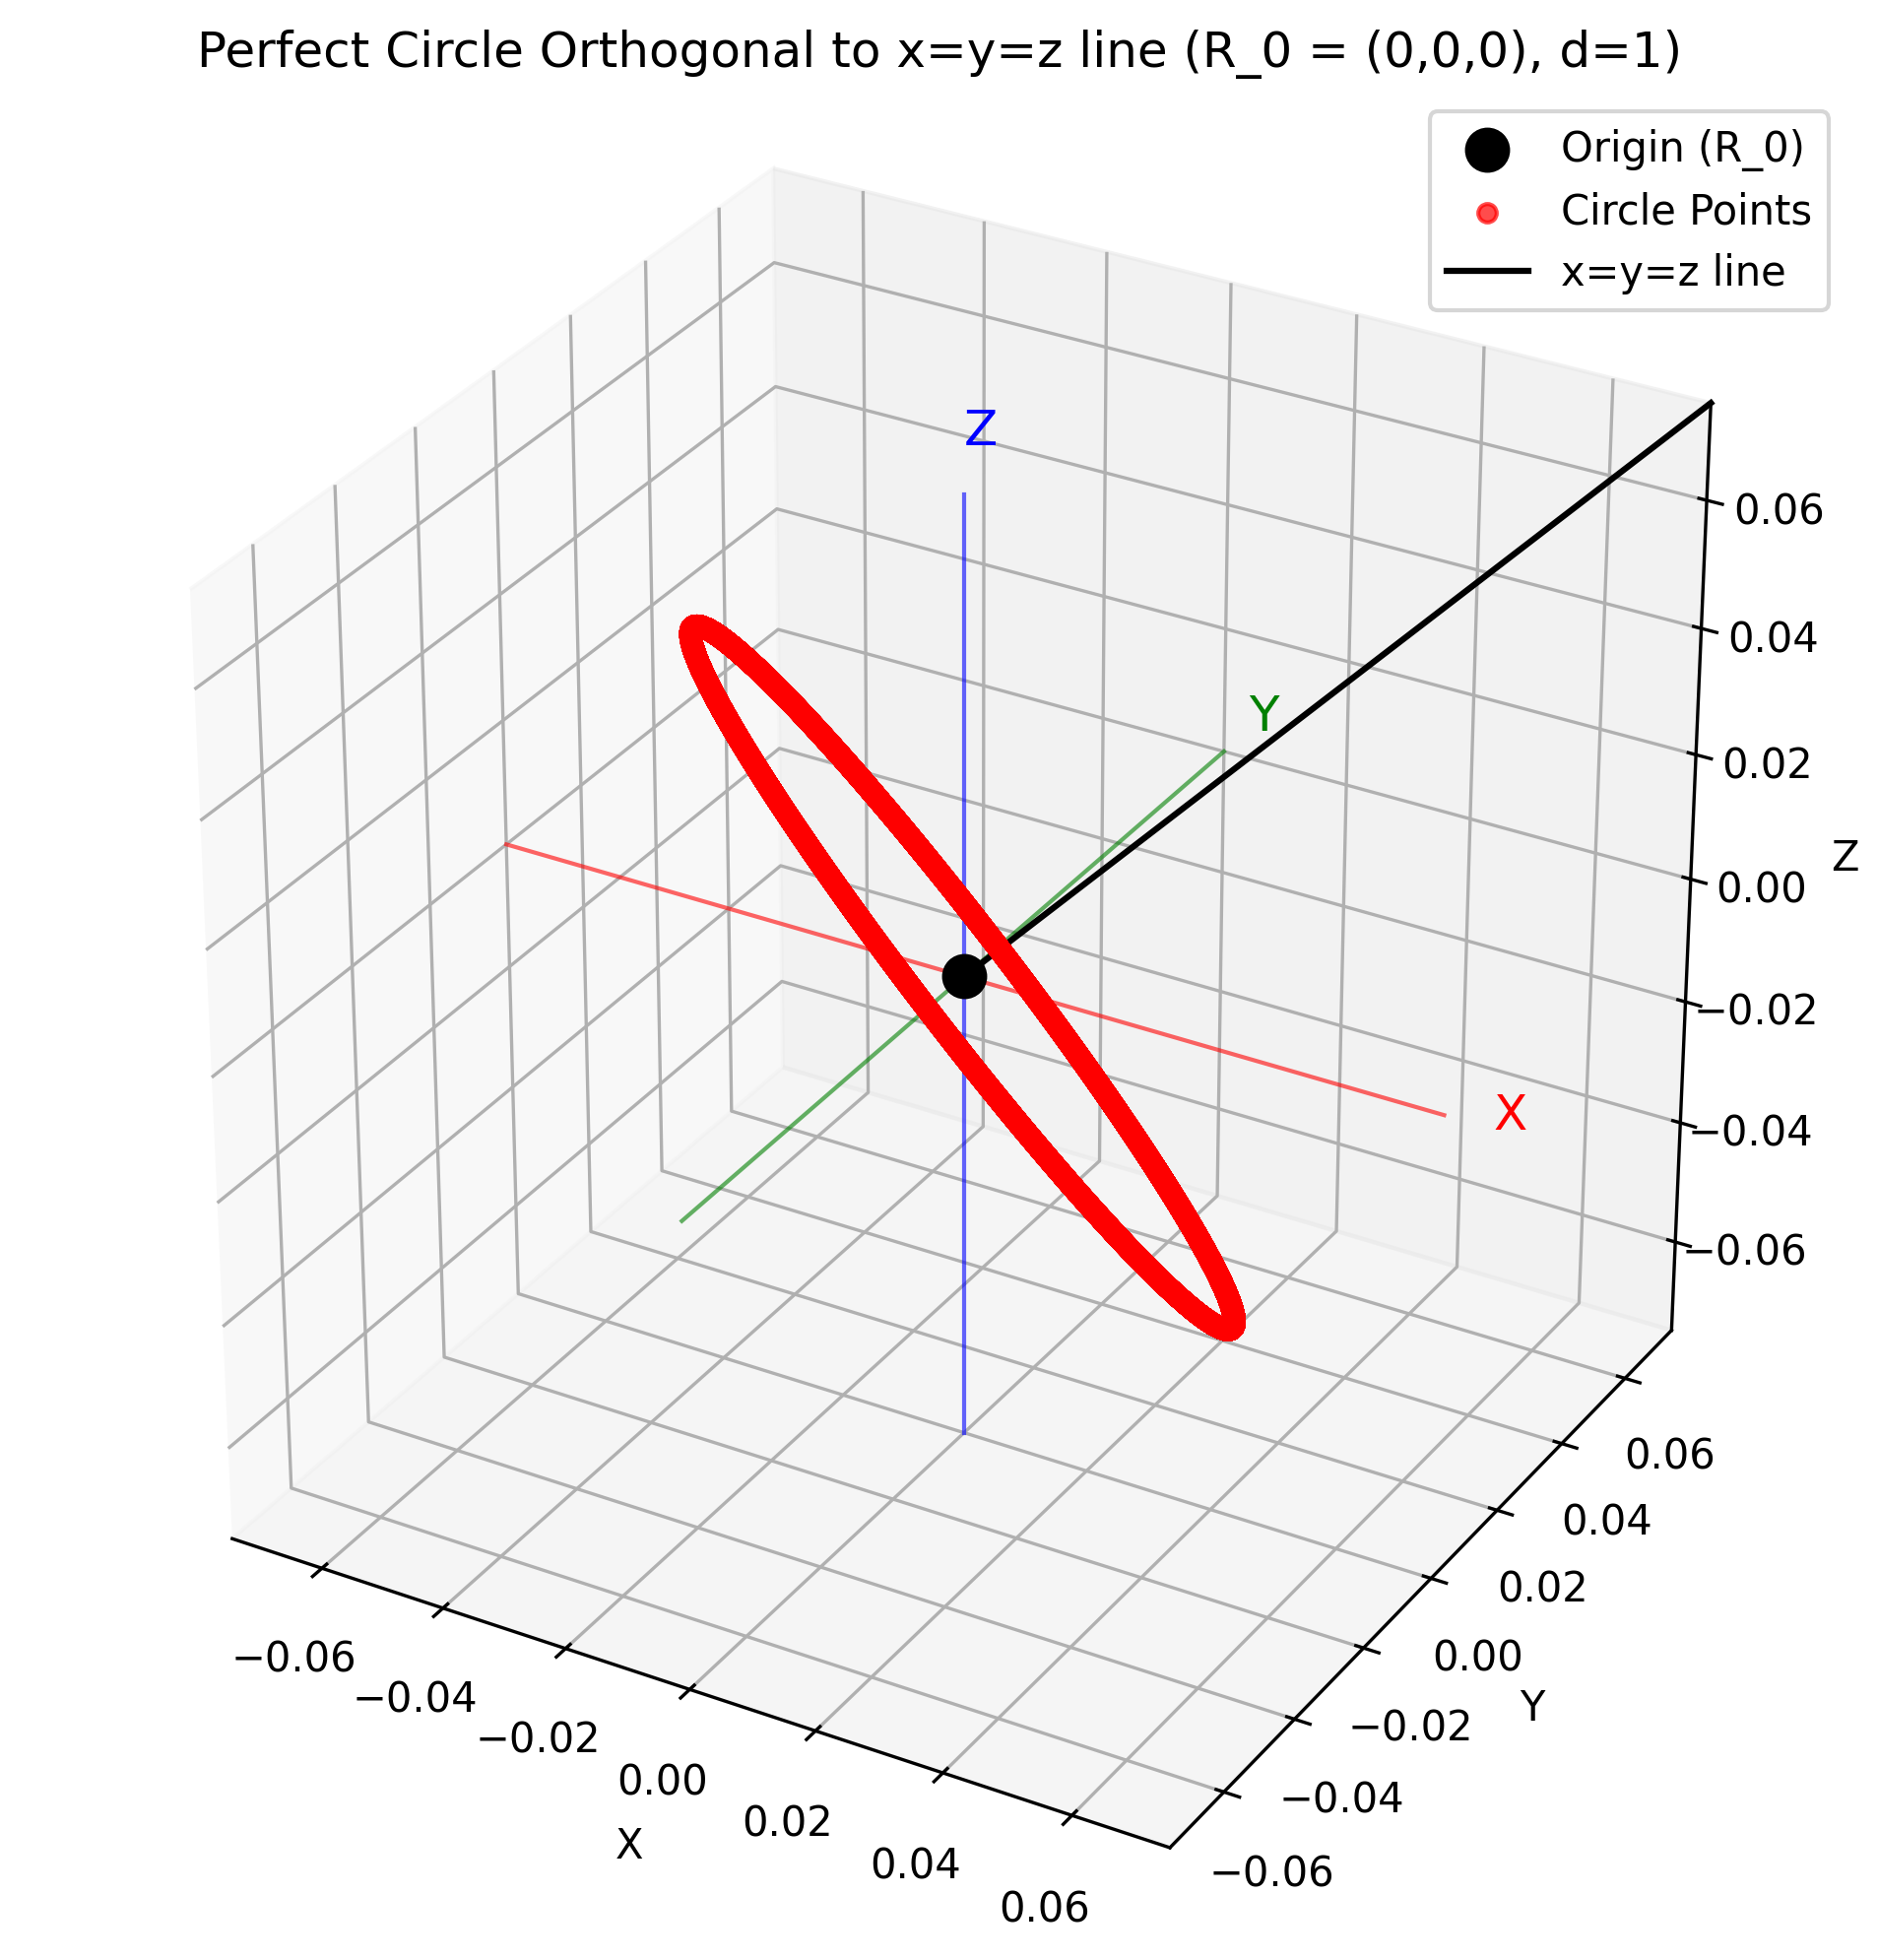
\includegraphics[width=0.8\textwidth]{../../../perfect_circle_output/perfect_circle_3d.png}
    \caption{3D visualization of the perfect circle orthogonal to the x=y=z line}
    \label{fig:perfect_circle_3d}
\end{figure}

\begin{figure}[H]
    \centering
    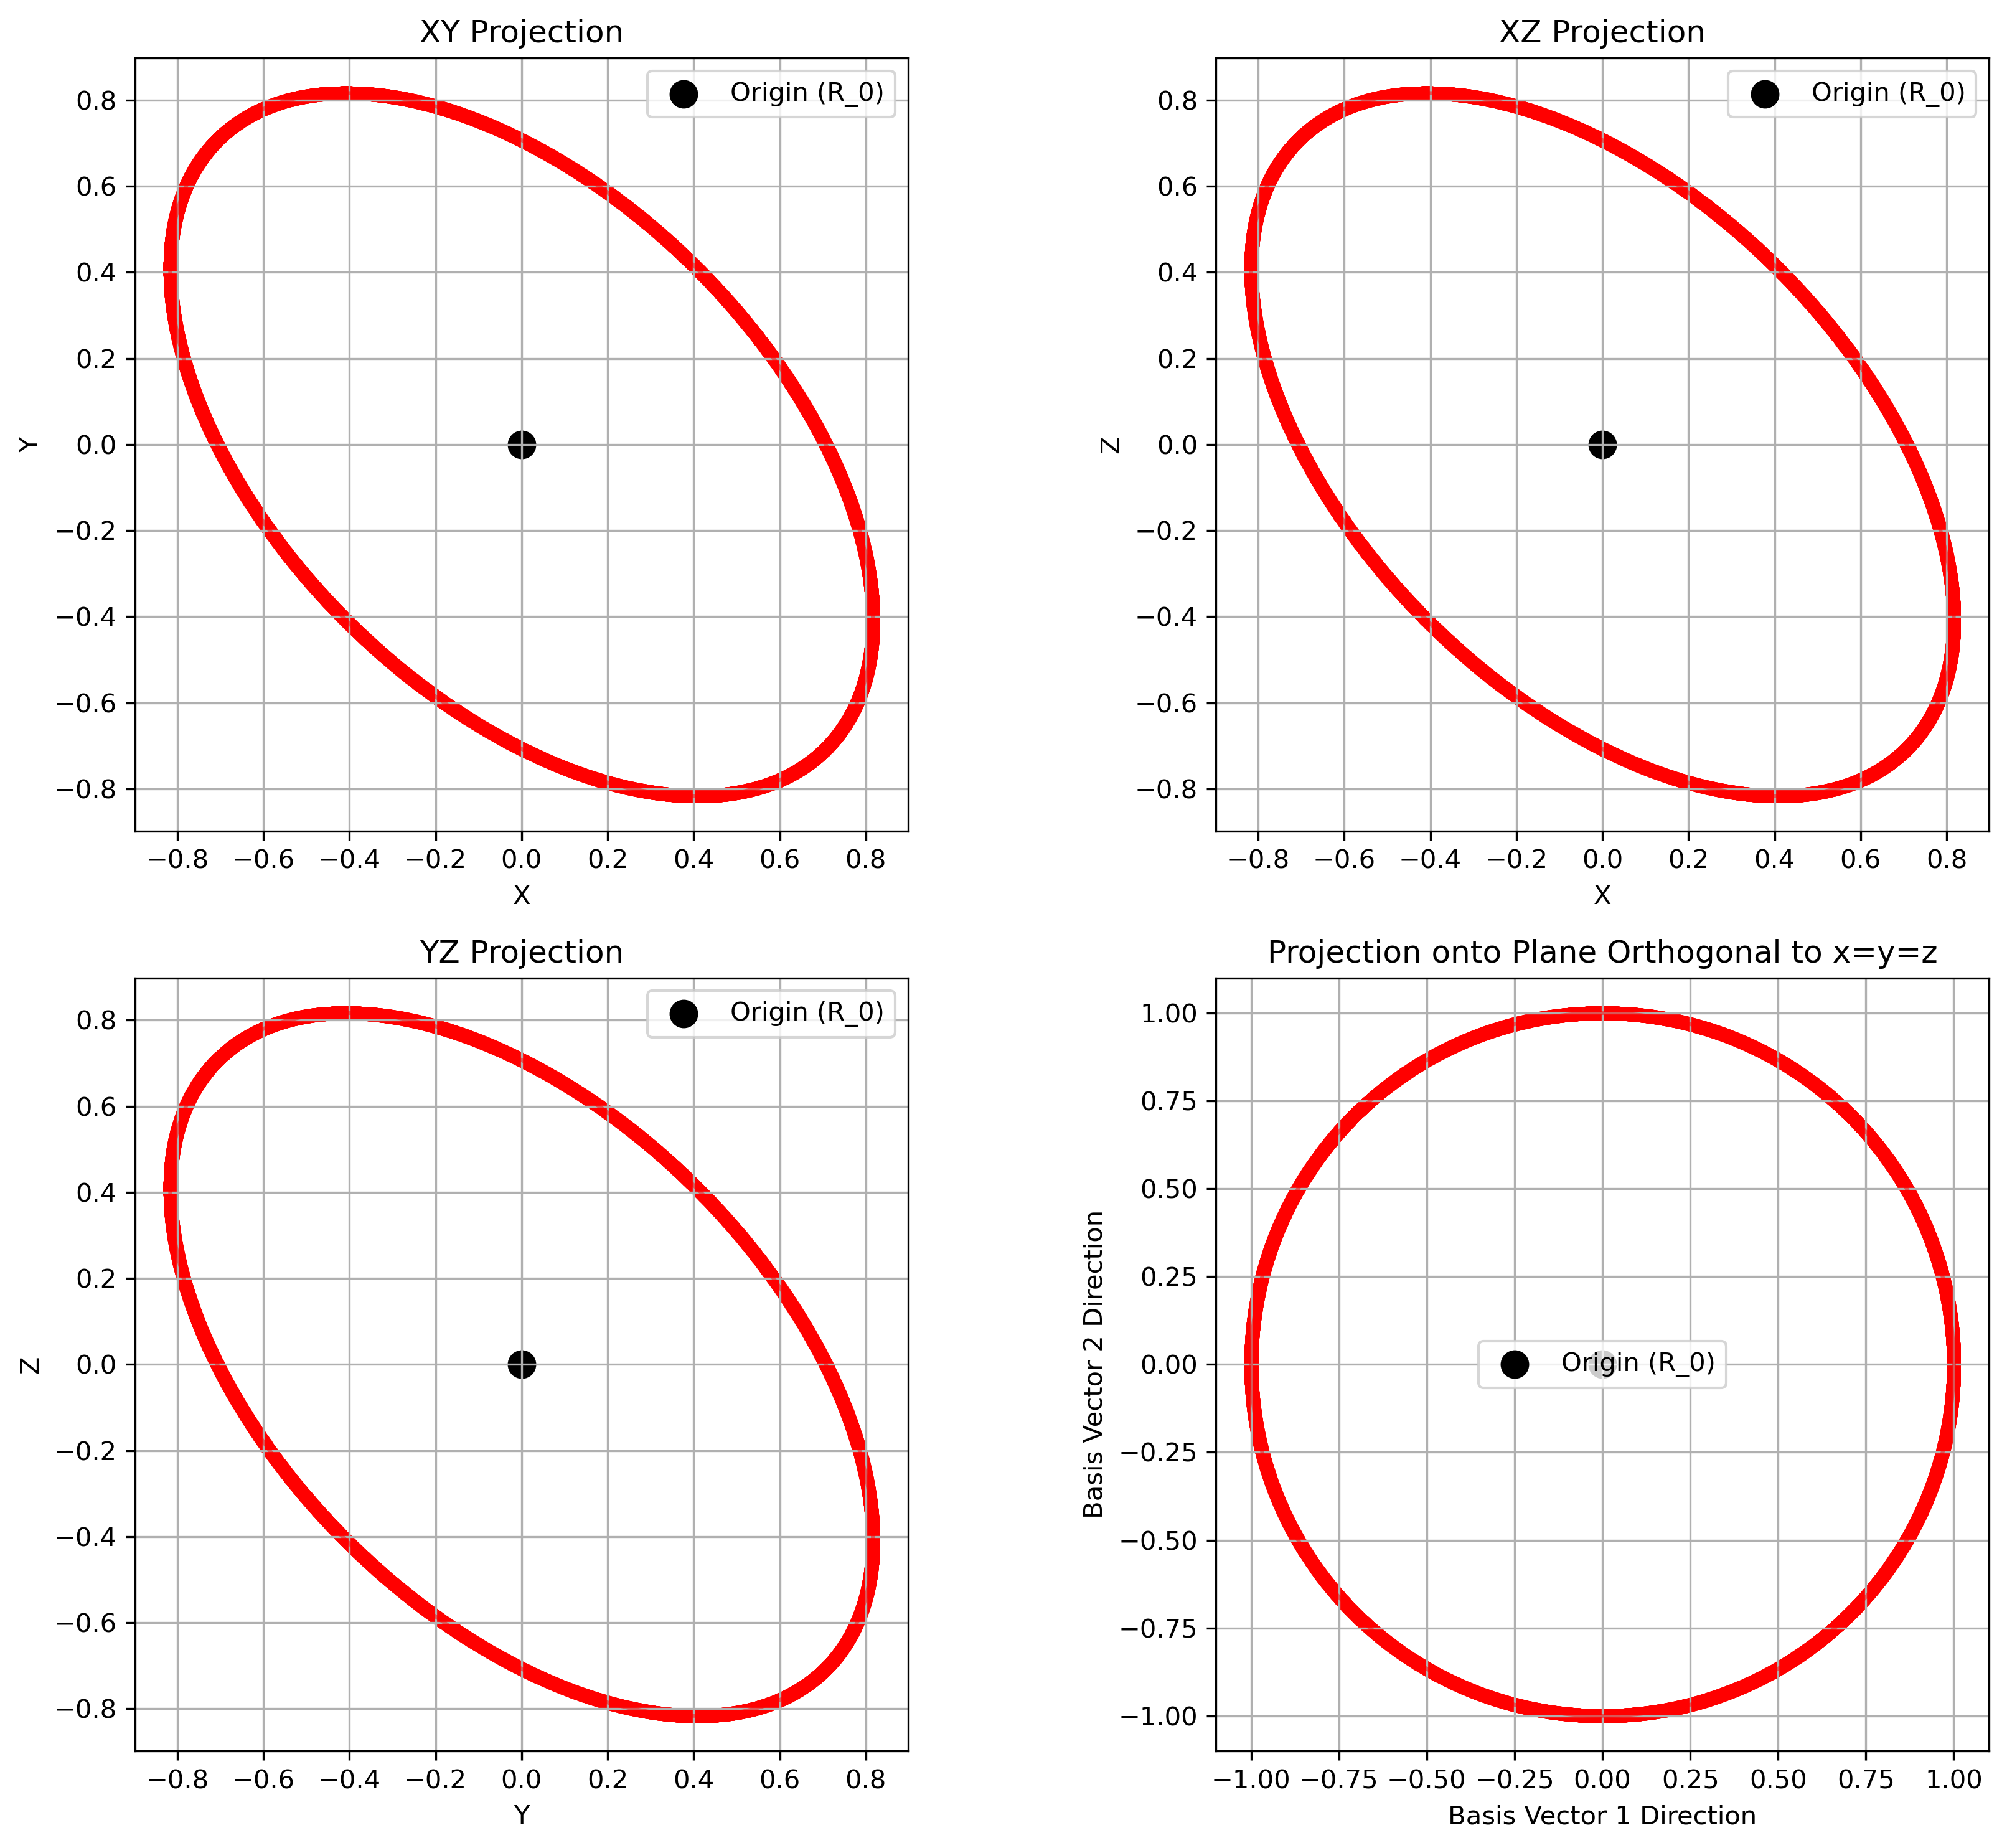
\includegraphics[width=0.8\textwidth]{../../../perfect_circle_output/perfect_circle_projections.png}
    \caption{Projections of the perfect circle onto coordinate planes and orthogonal plane}
    \label{fig:perfect_circle_projections}
\end{figure}

\begin{figure}[H]
    \centering
    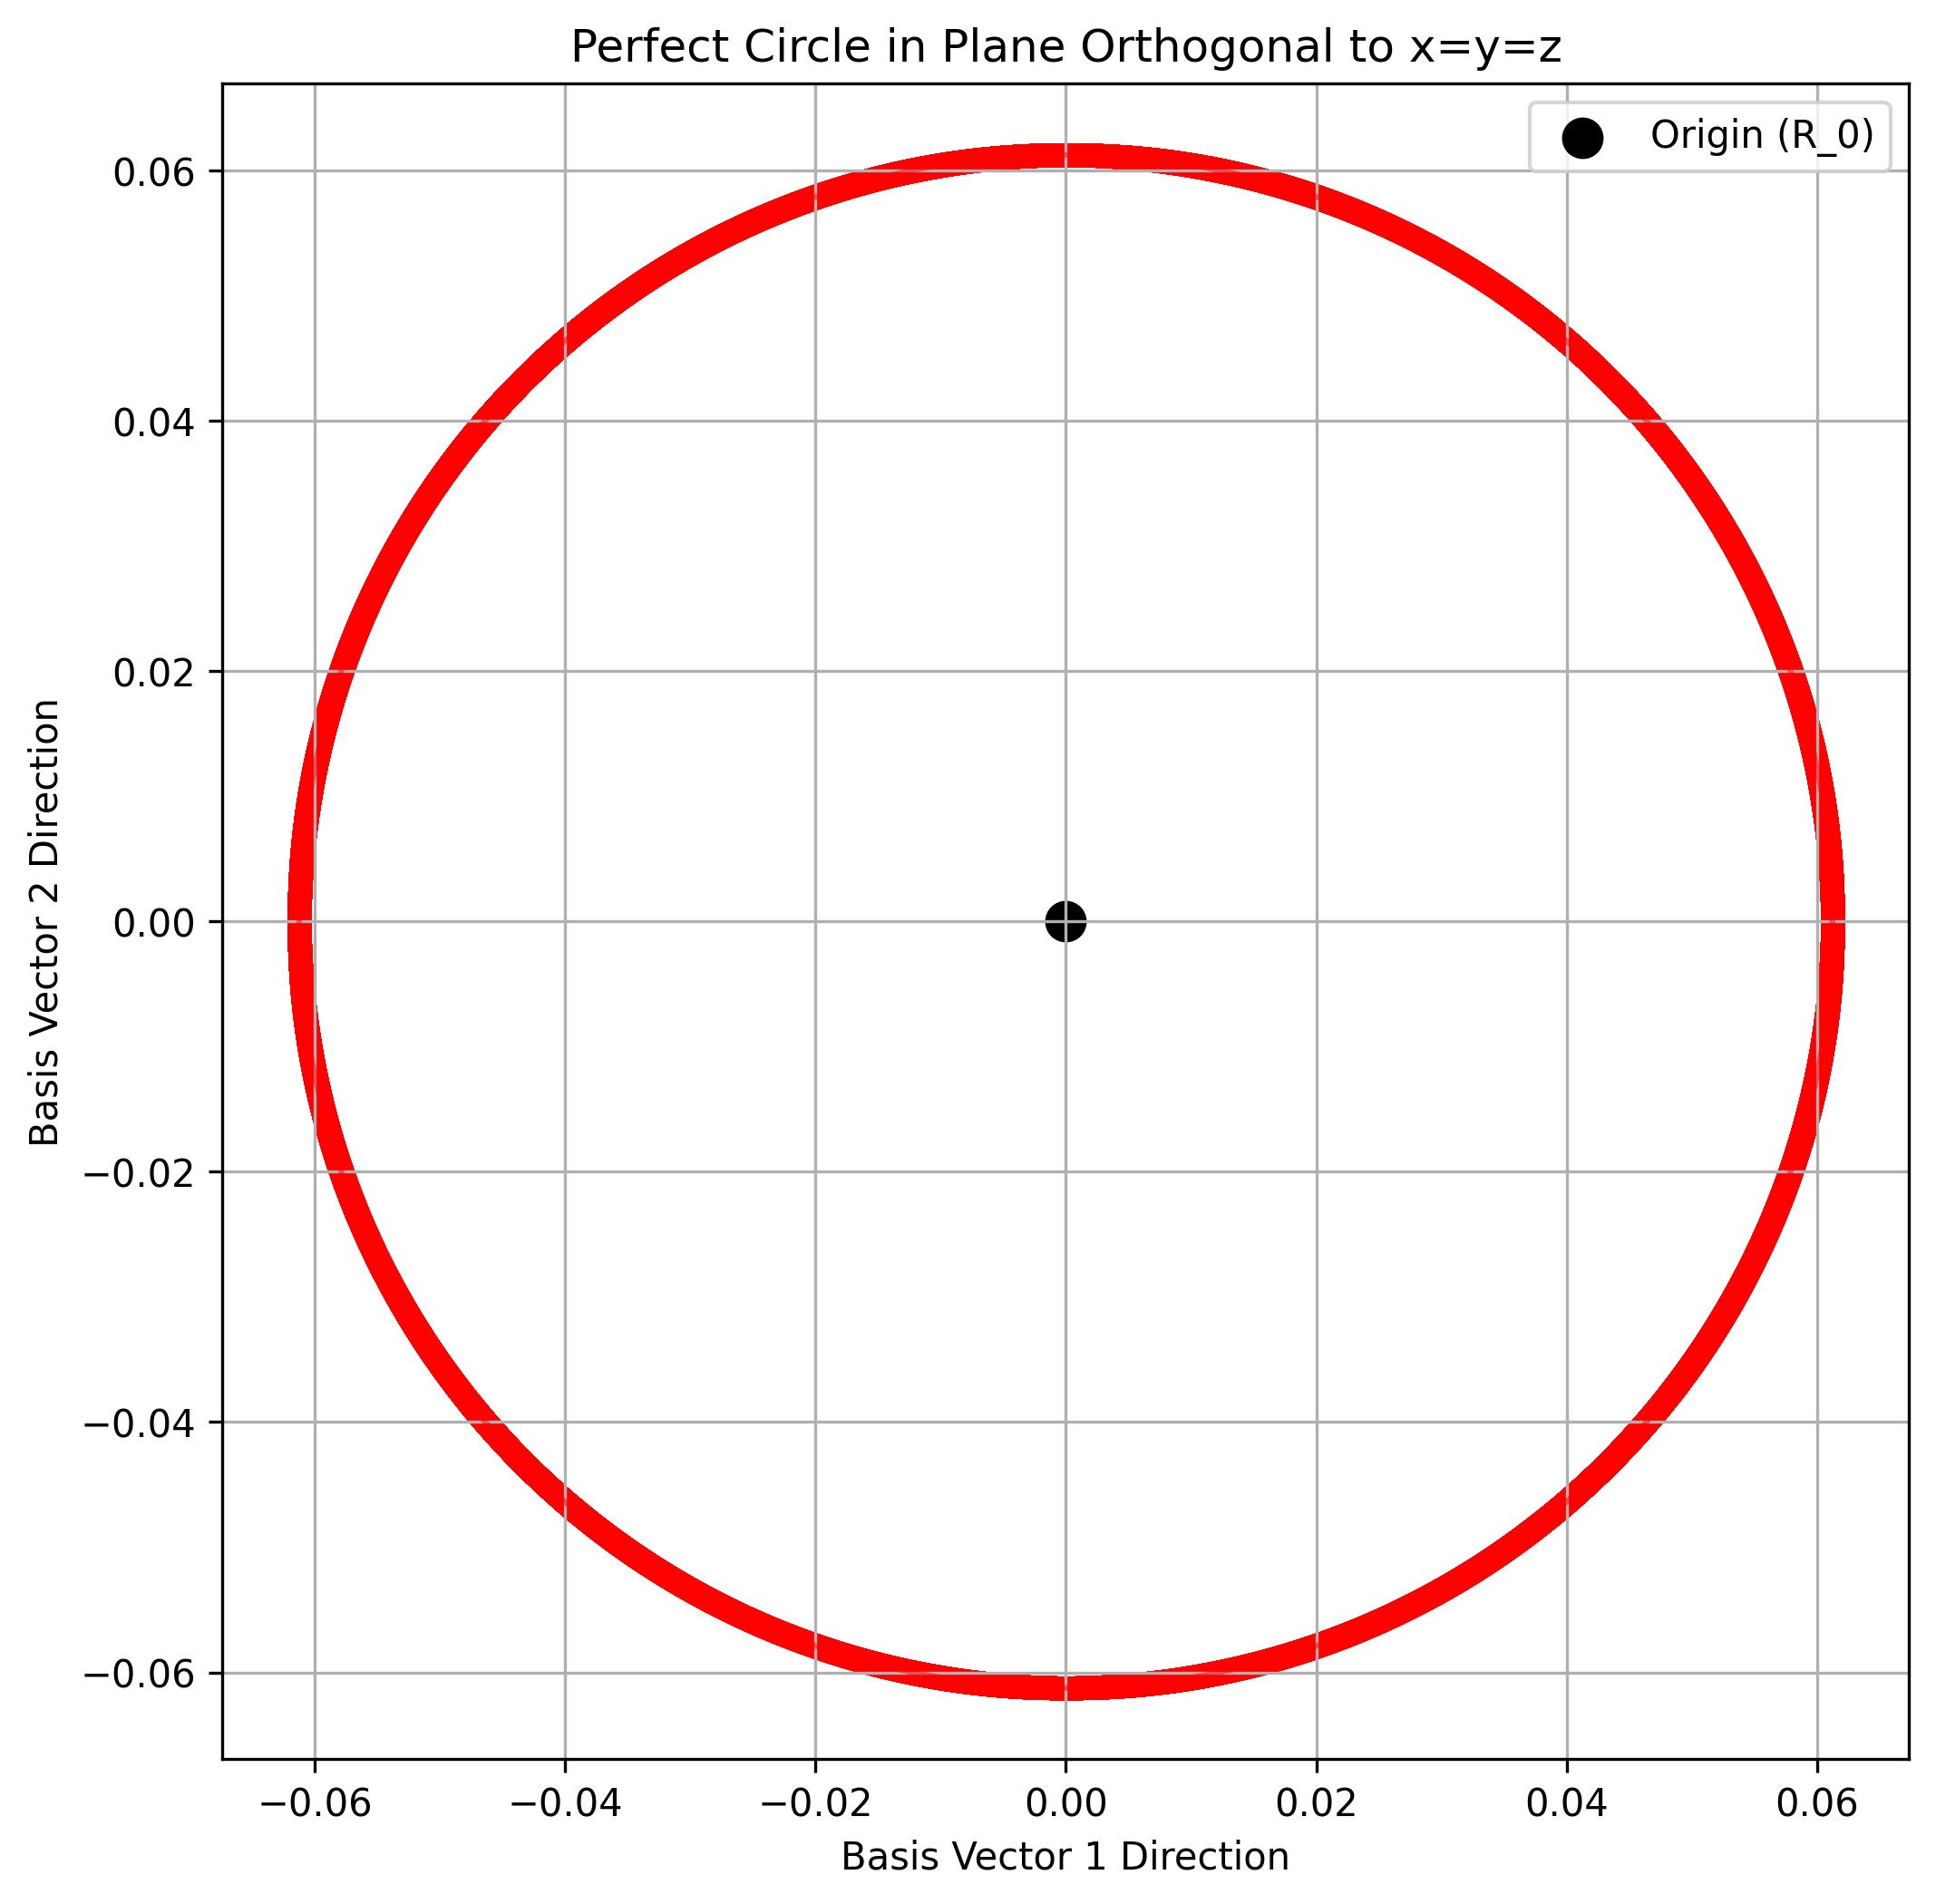
\includegraphics[width=0.8\textwidth]{../../../perfect_circle_output/perfect_circle_orthogonal_plane.png}
    \caption{Perfect circle projected onto the plane orthogonal to the x=y=z line}
    \label{fig:perfect_circle_orthogonal}
\end{figure}

\subsection{Orthogonality Test Results}

This section presents the results of comprehensive tests verifying the orthogonality of generated vectors to the x=y=z line. These tests confirm that the implementation using basis vectors correctly ensures orthogonality to the (1,1,1) direction.

\subsubsection{Single Vector Orthogonality Test}

A test was conducted with the following parameters:
\begin{itemize}
    \item Origin vector (R\_0): [1, 1, 1]
    \item Distance parameter (d): 2.0
    \item Angle parameter ($\theta$): $\pi/4$ (45 degrees)
\end{itemize}

The test verified that the displacement vector (R - R\_0) is orthogonal to the (1,1,1) direction by calculating the dot product, which was effectively zero (within floating-point precision).

\begin{figure}[H]
    \centering
    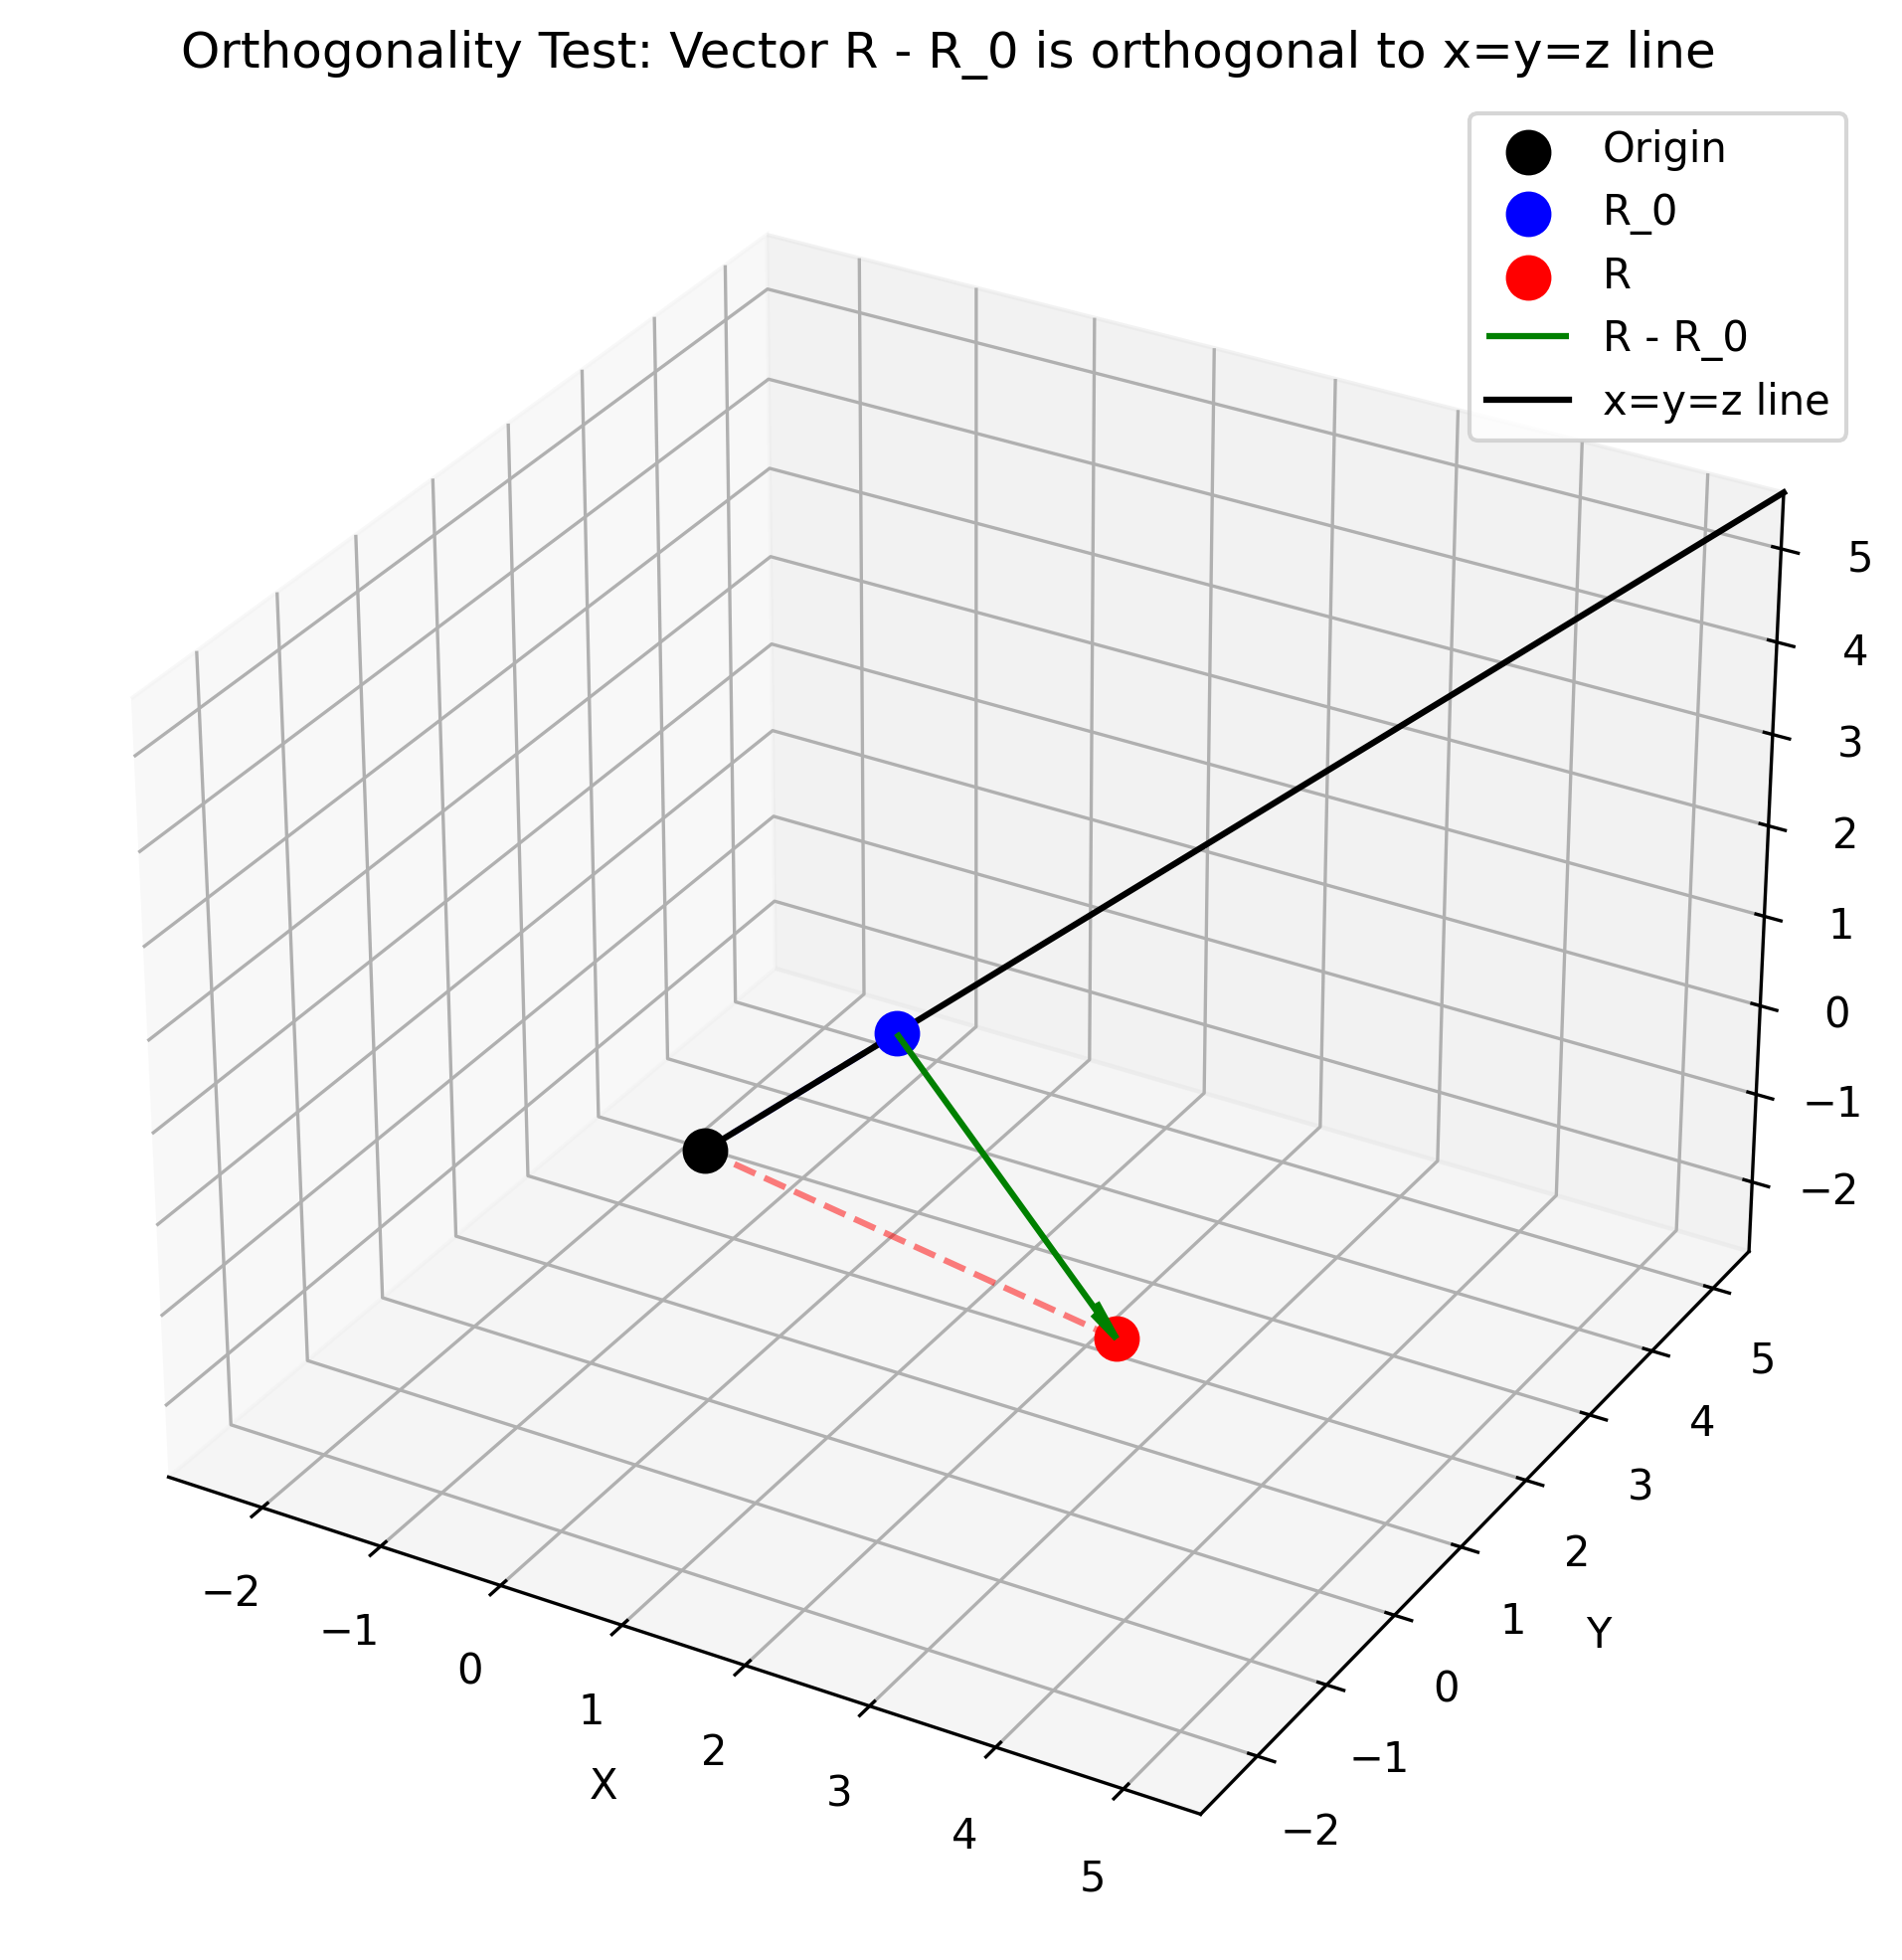
\includegraphics[width=0.8\textwidth]{figures/orthogonality_test/orthogonality_test_3d.png}
    \caption{3D visualization showing the orthogonality of the displacement vector to the x=y=z line}
    \label{fig:orthogonality_test_3d}
\end{figure}

\begin{figure}[H]
    \centering
    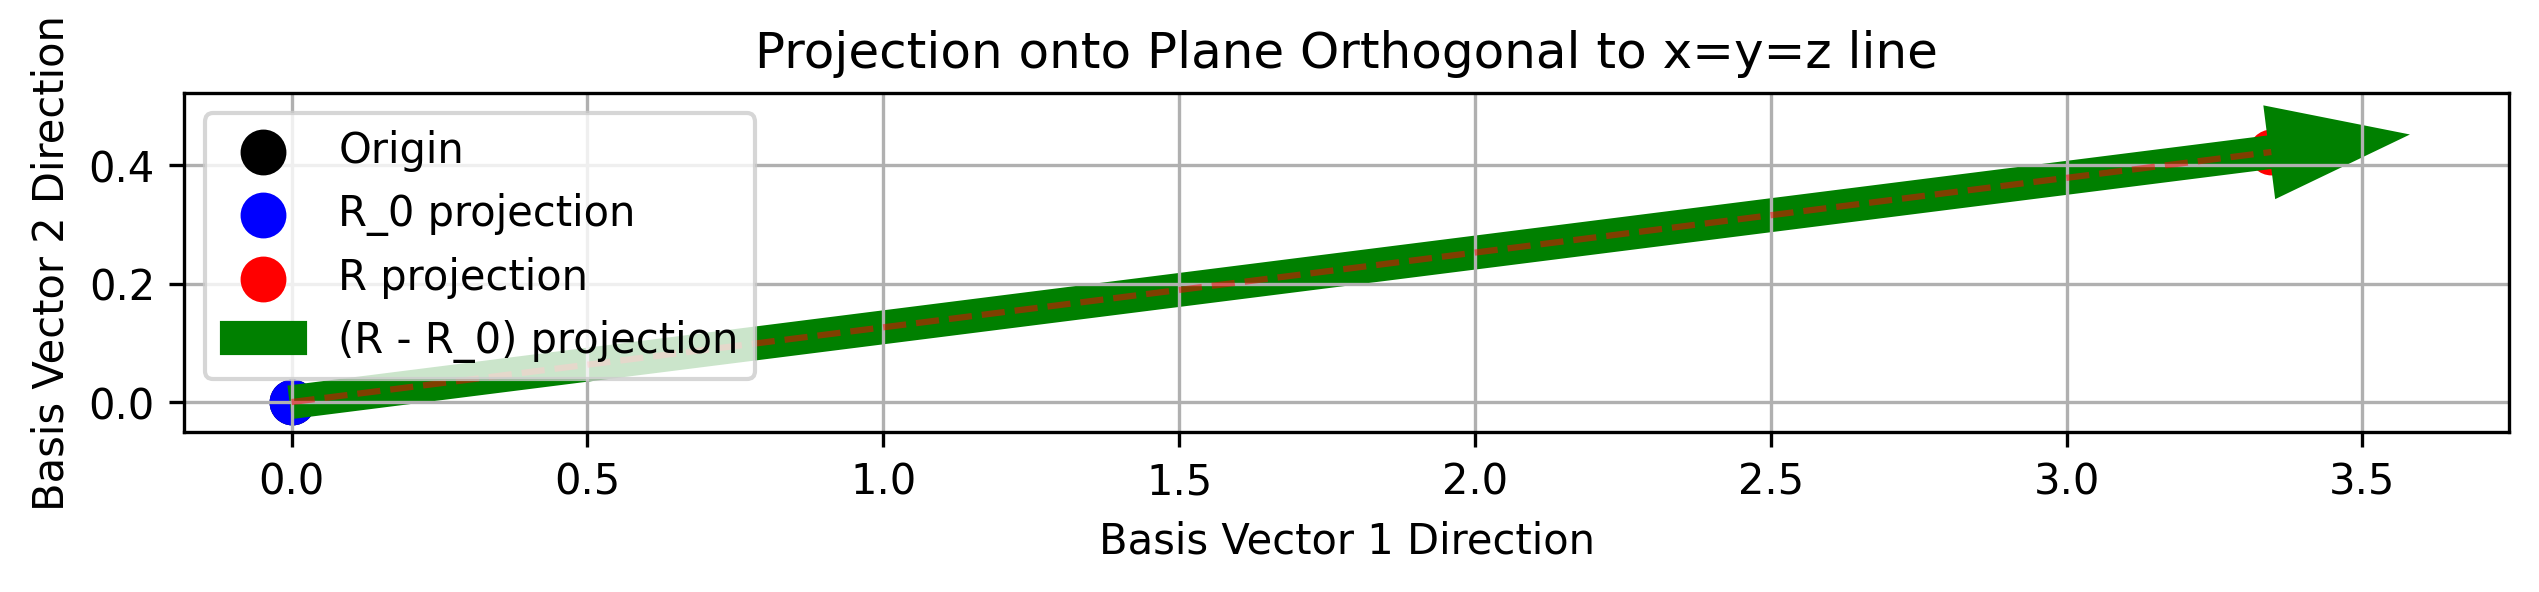
\includegraphics[width=0.8\textwidth]{figures/orthogonality_test/orthogonality_test_2d.png}
    \caption{2D projection onto the plane orthogonal to the x=y=z line}
    \label{fig:orthogonality_test_2d}
\end{figure}

\subsubsection{Circle Orthogonality Test}

A test was conducted to verify that vectors generated by varying $\theta$ from 0 to $2\pi$ form a circle in the plane orthogonal to the x=y=z line. The test used 73 points (5-degree increments) and confirmed that all generated vectors maintain orthogonality to the (1,1,1) direction.

\begin{figure}[H]
    \centering
    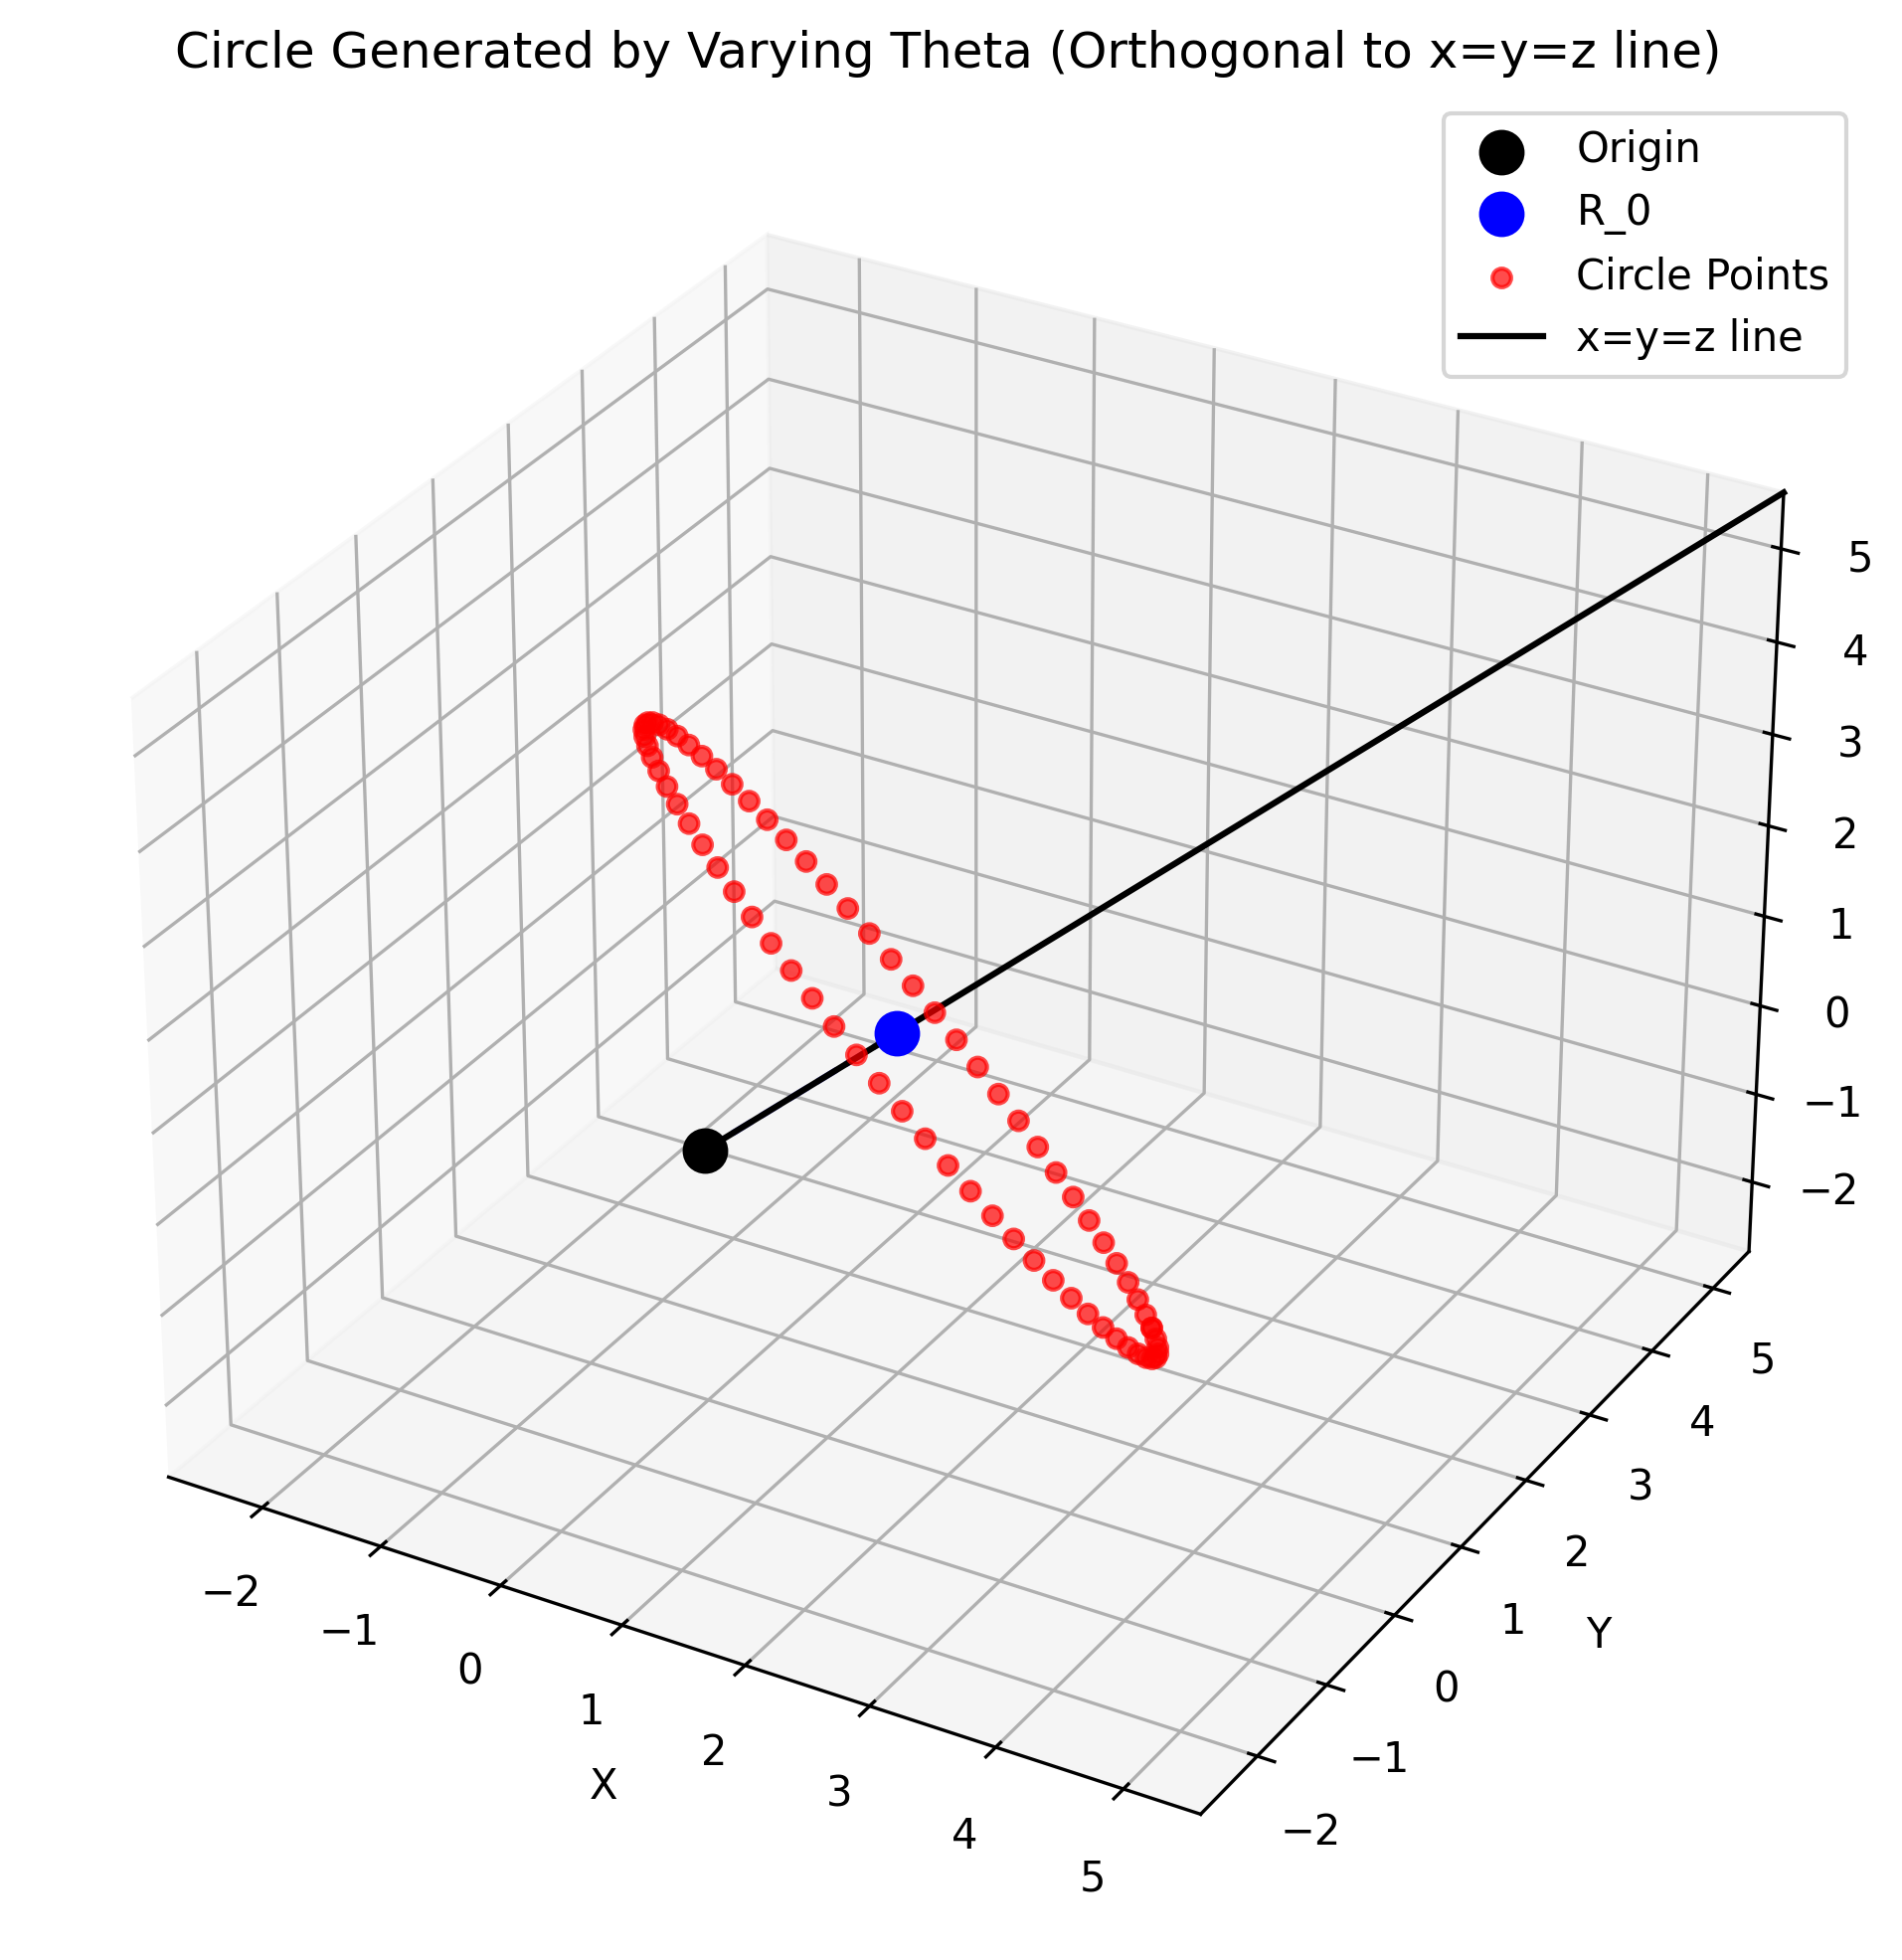
\includegraphics[width=0.8\textwidth]{figures/orthogonality_test/orthogonality_circle_3d.png}
    \caption{3D visualization of the circle formed by vectors orthogonal to the x=y=z line}
    \label{fig:orthogonality_circle_3d}
\end{figure}

\begin{figure}[H]
    \centering
    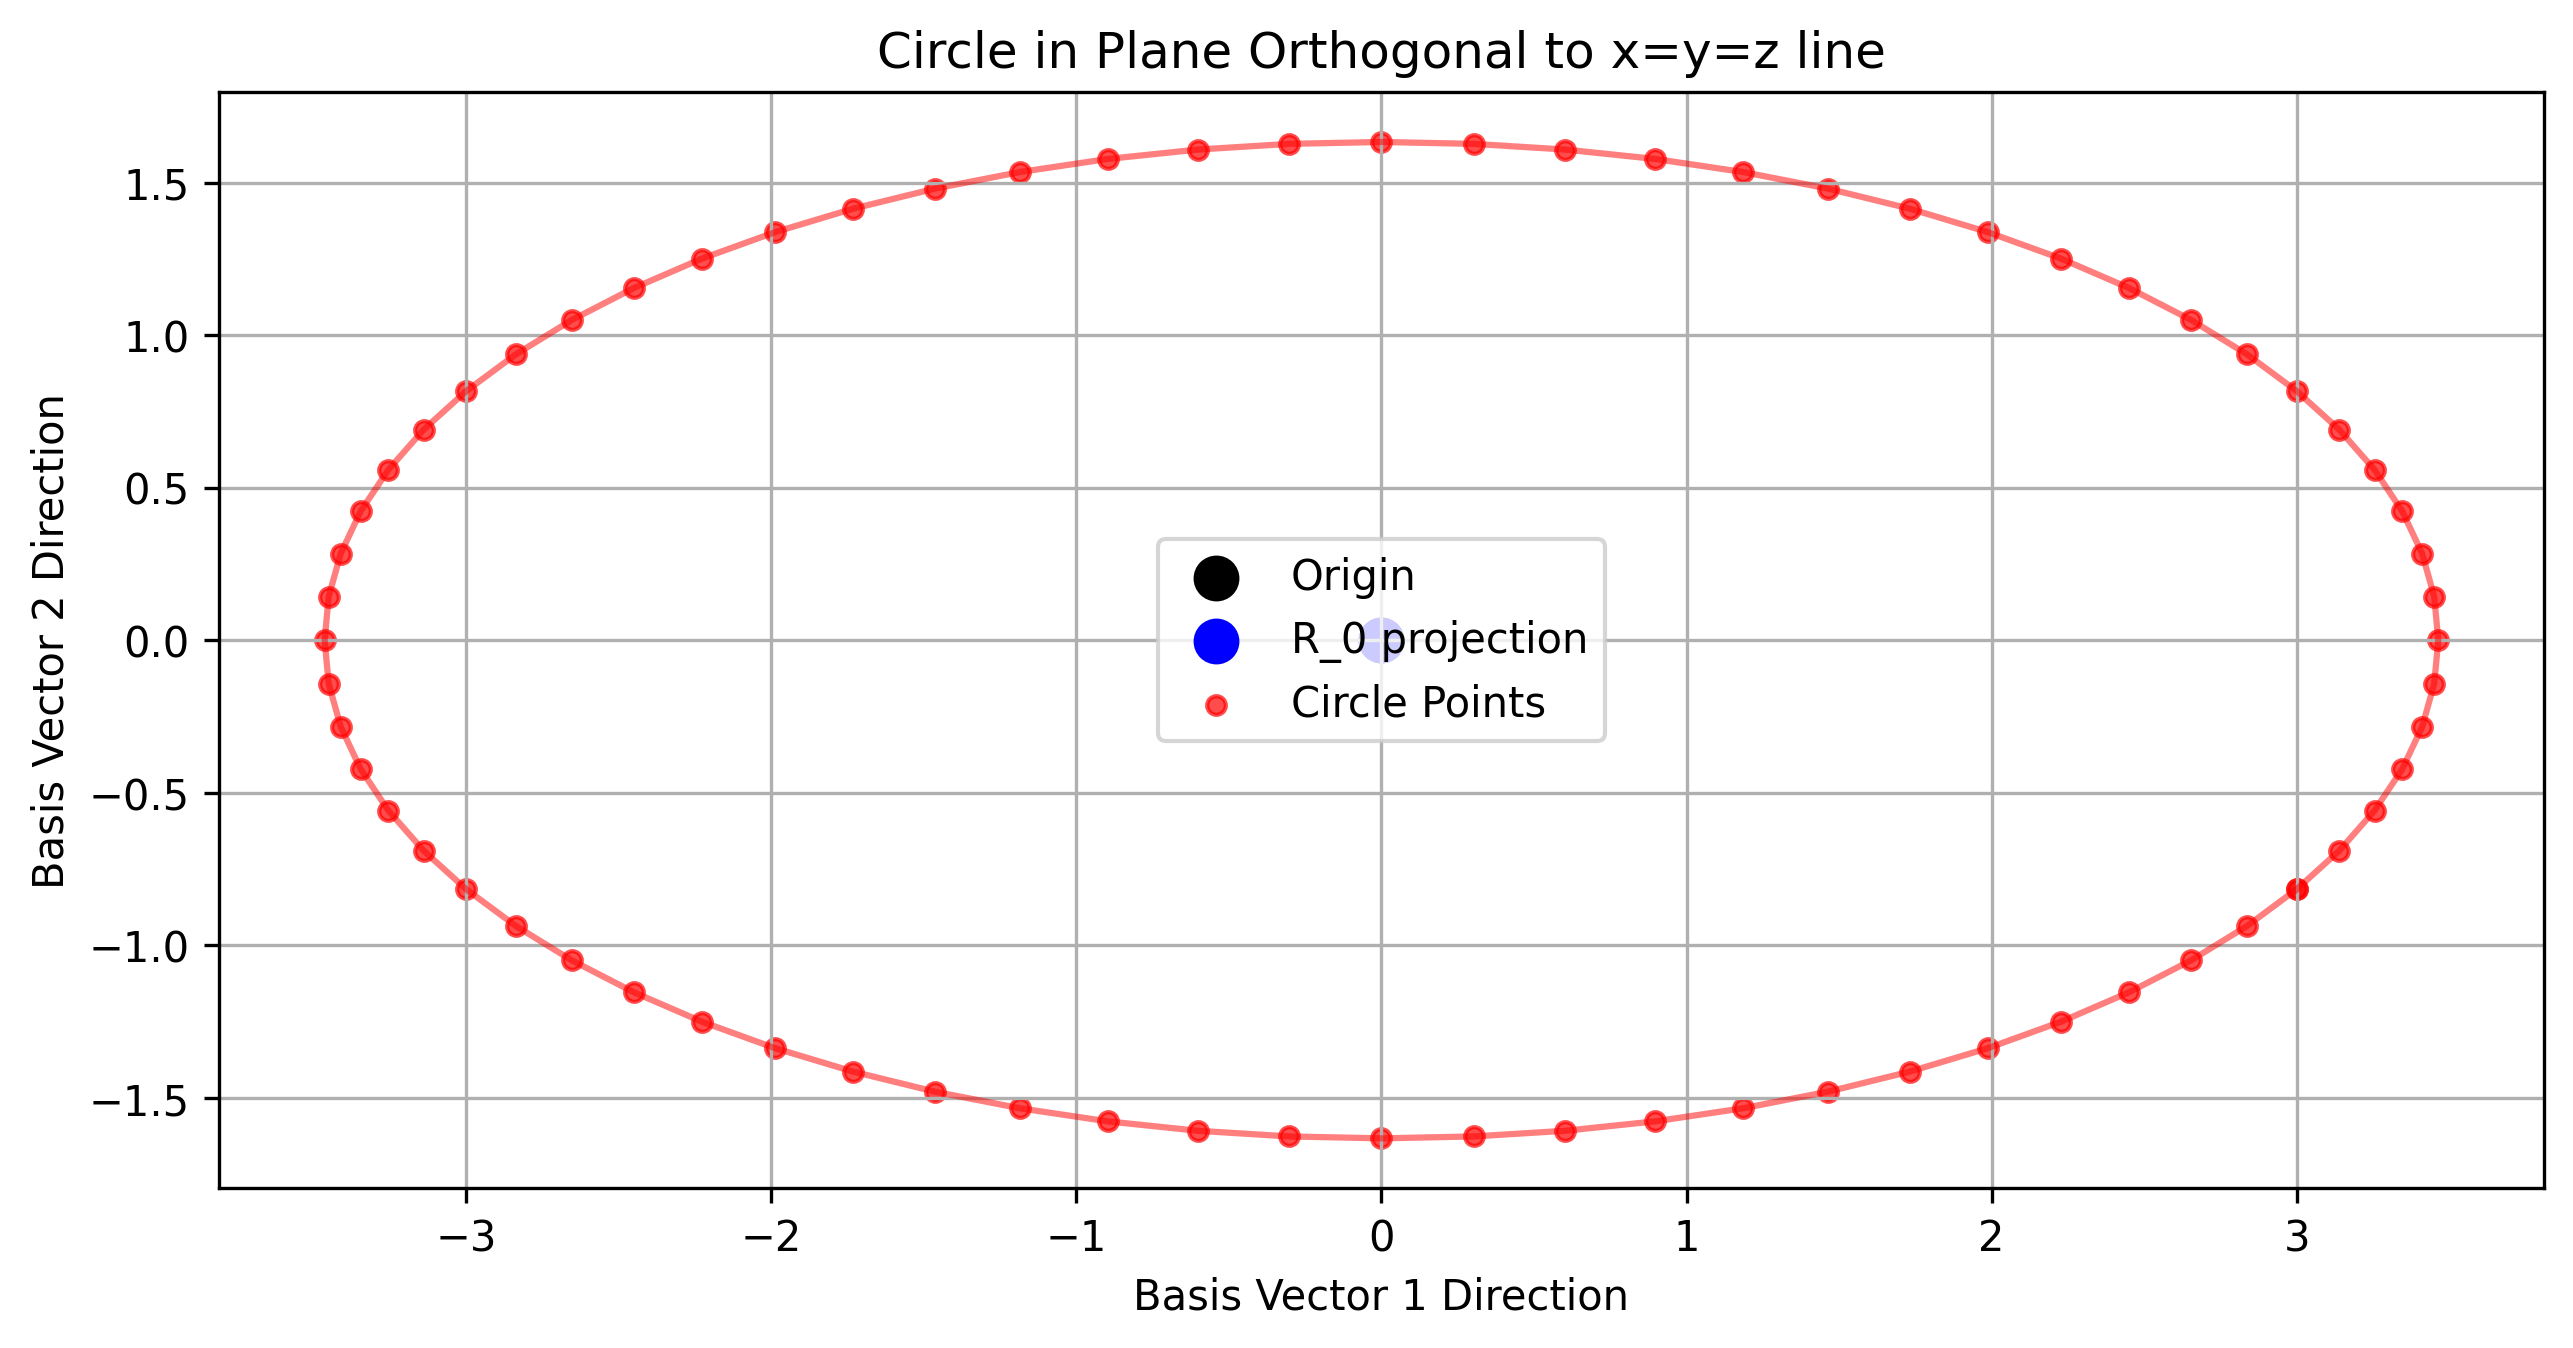
\includegraphics[width=0.8\textwidth]{figures/orthogonality_test/orthogonality_circle_2d.png}
    \caption{2D projection of the circle onto the plane orthogonal to the x=y=z line}
    \label{fig:orthogonality_circle_2d}
\end{figure}

\subsubsection{Comprehensive Circle Visualization}

A comprehensive visualization was created to show the circle from multiple perspectives:

\begin{figure}[H]
    \centering
    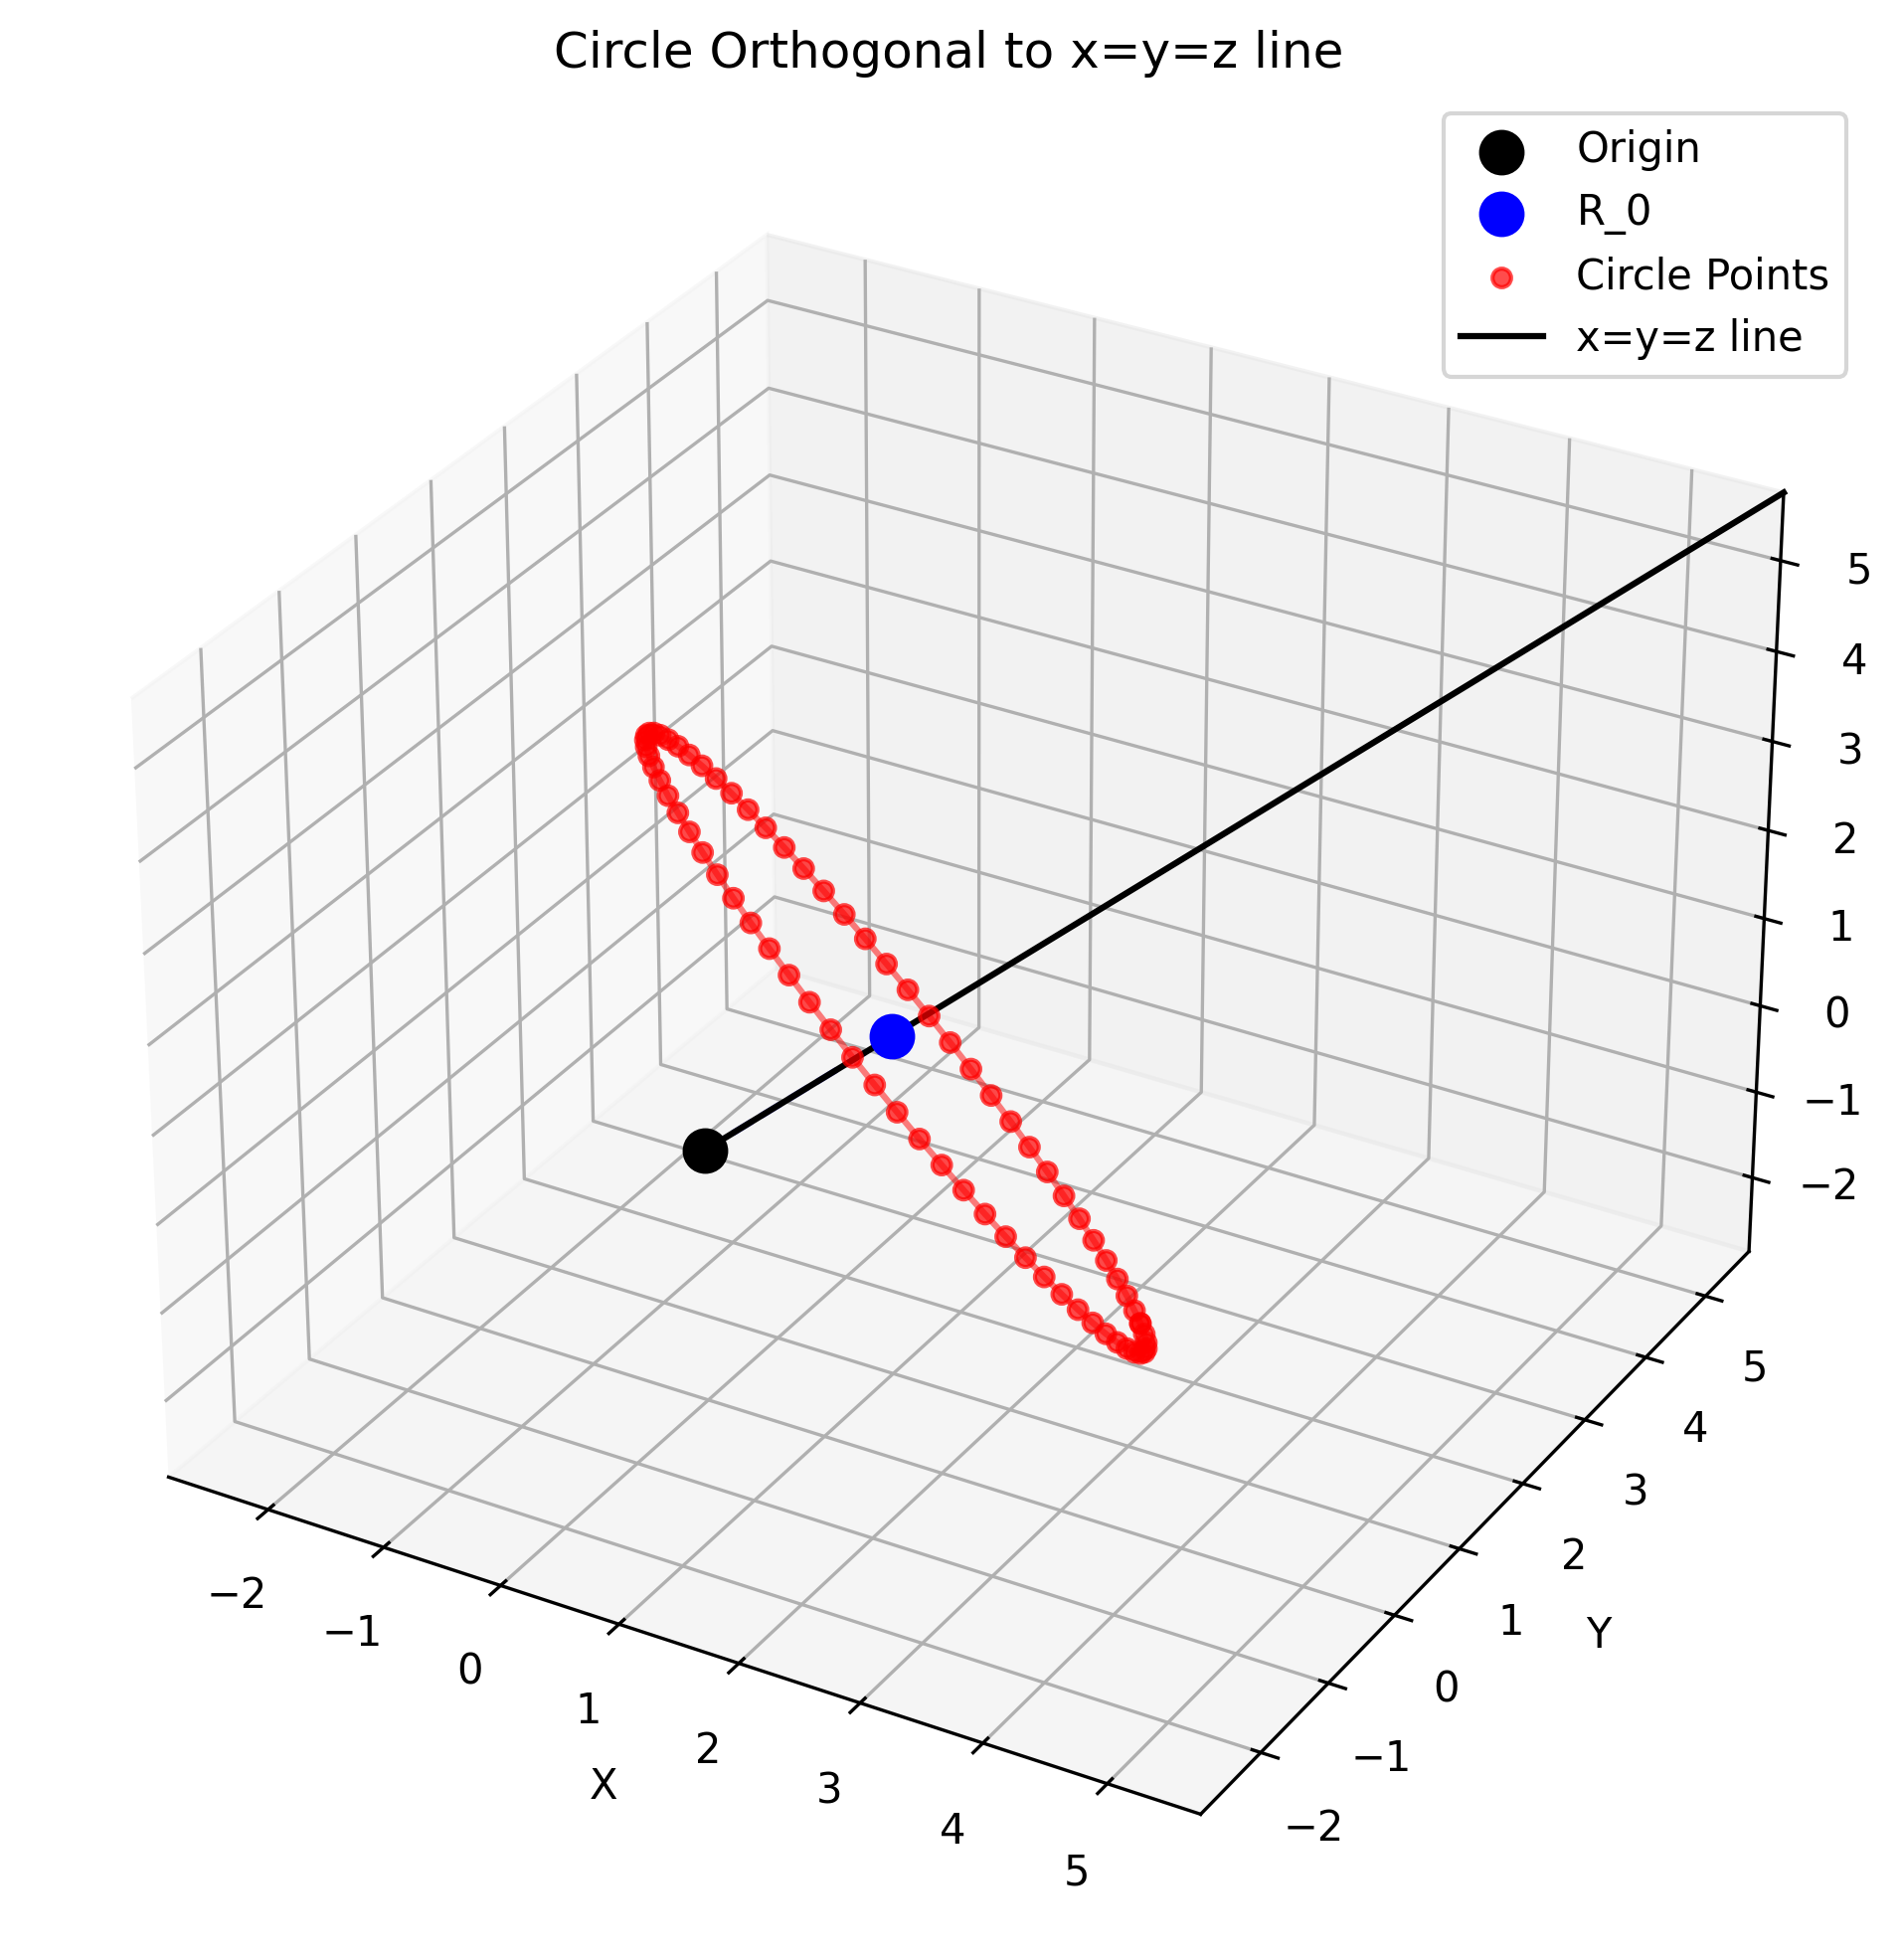
\includegraphics[width=0.8\textwidth]{figures/orthogonality_test/orthogonal_circle_3d.png}
    \caption{3D visualization of the circle orthogonal to the x=y=z line}
    \label{fig:orthogonal_circle_3d}
\end{figure}

\begin{figure}[H]
    \centering
    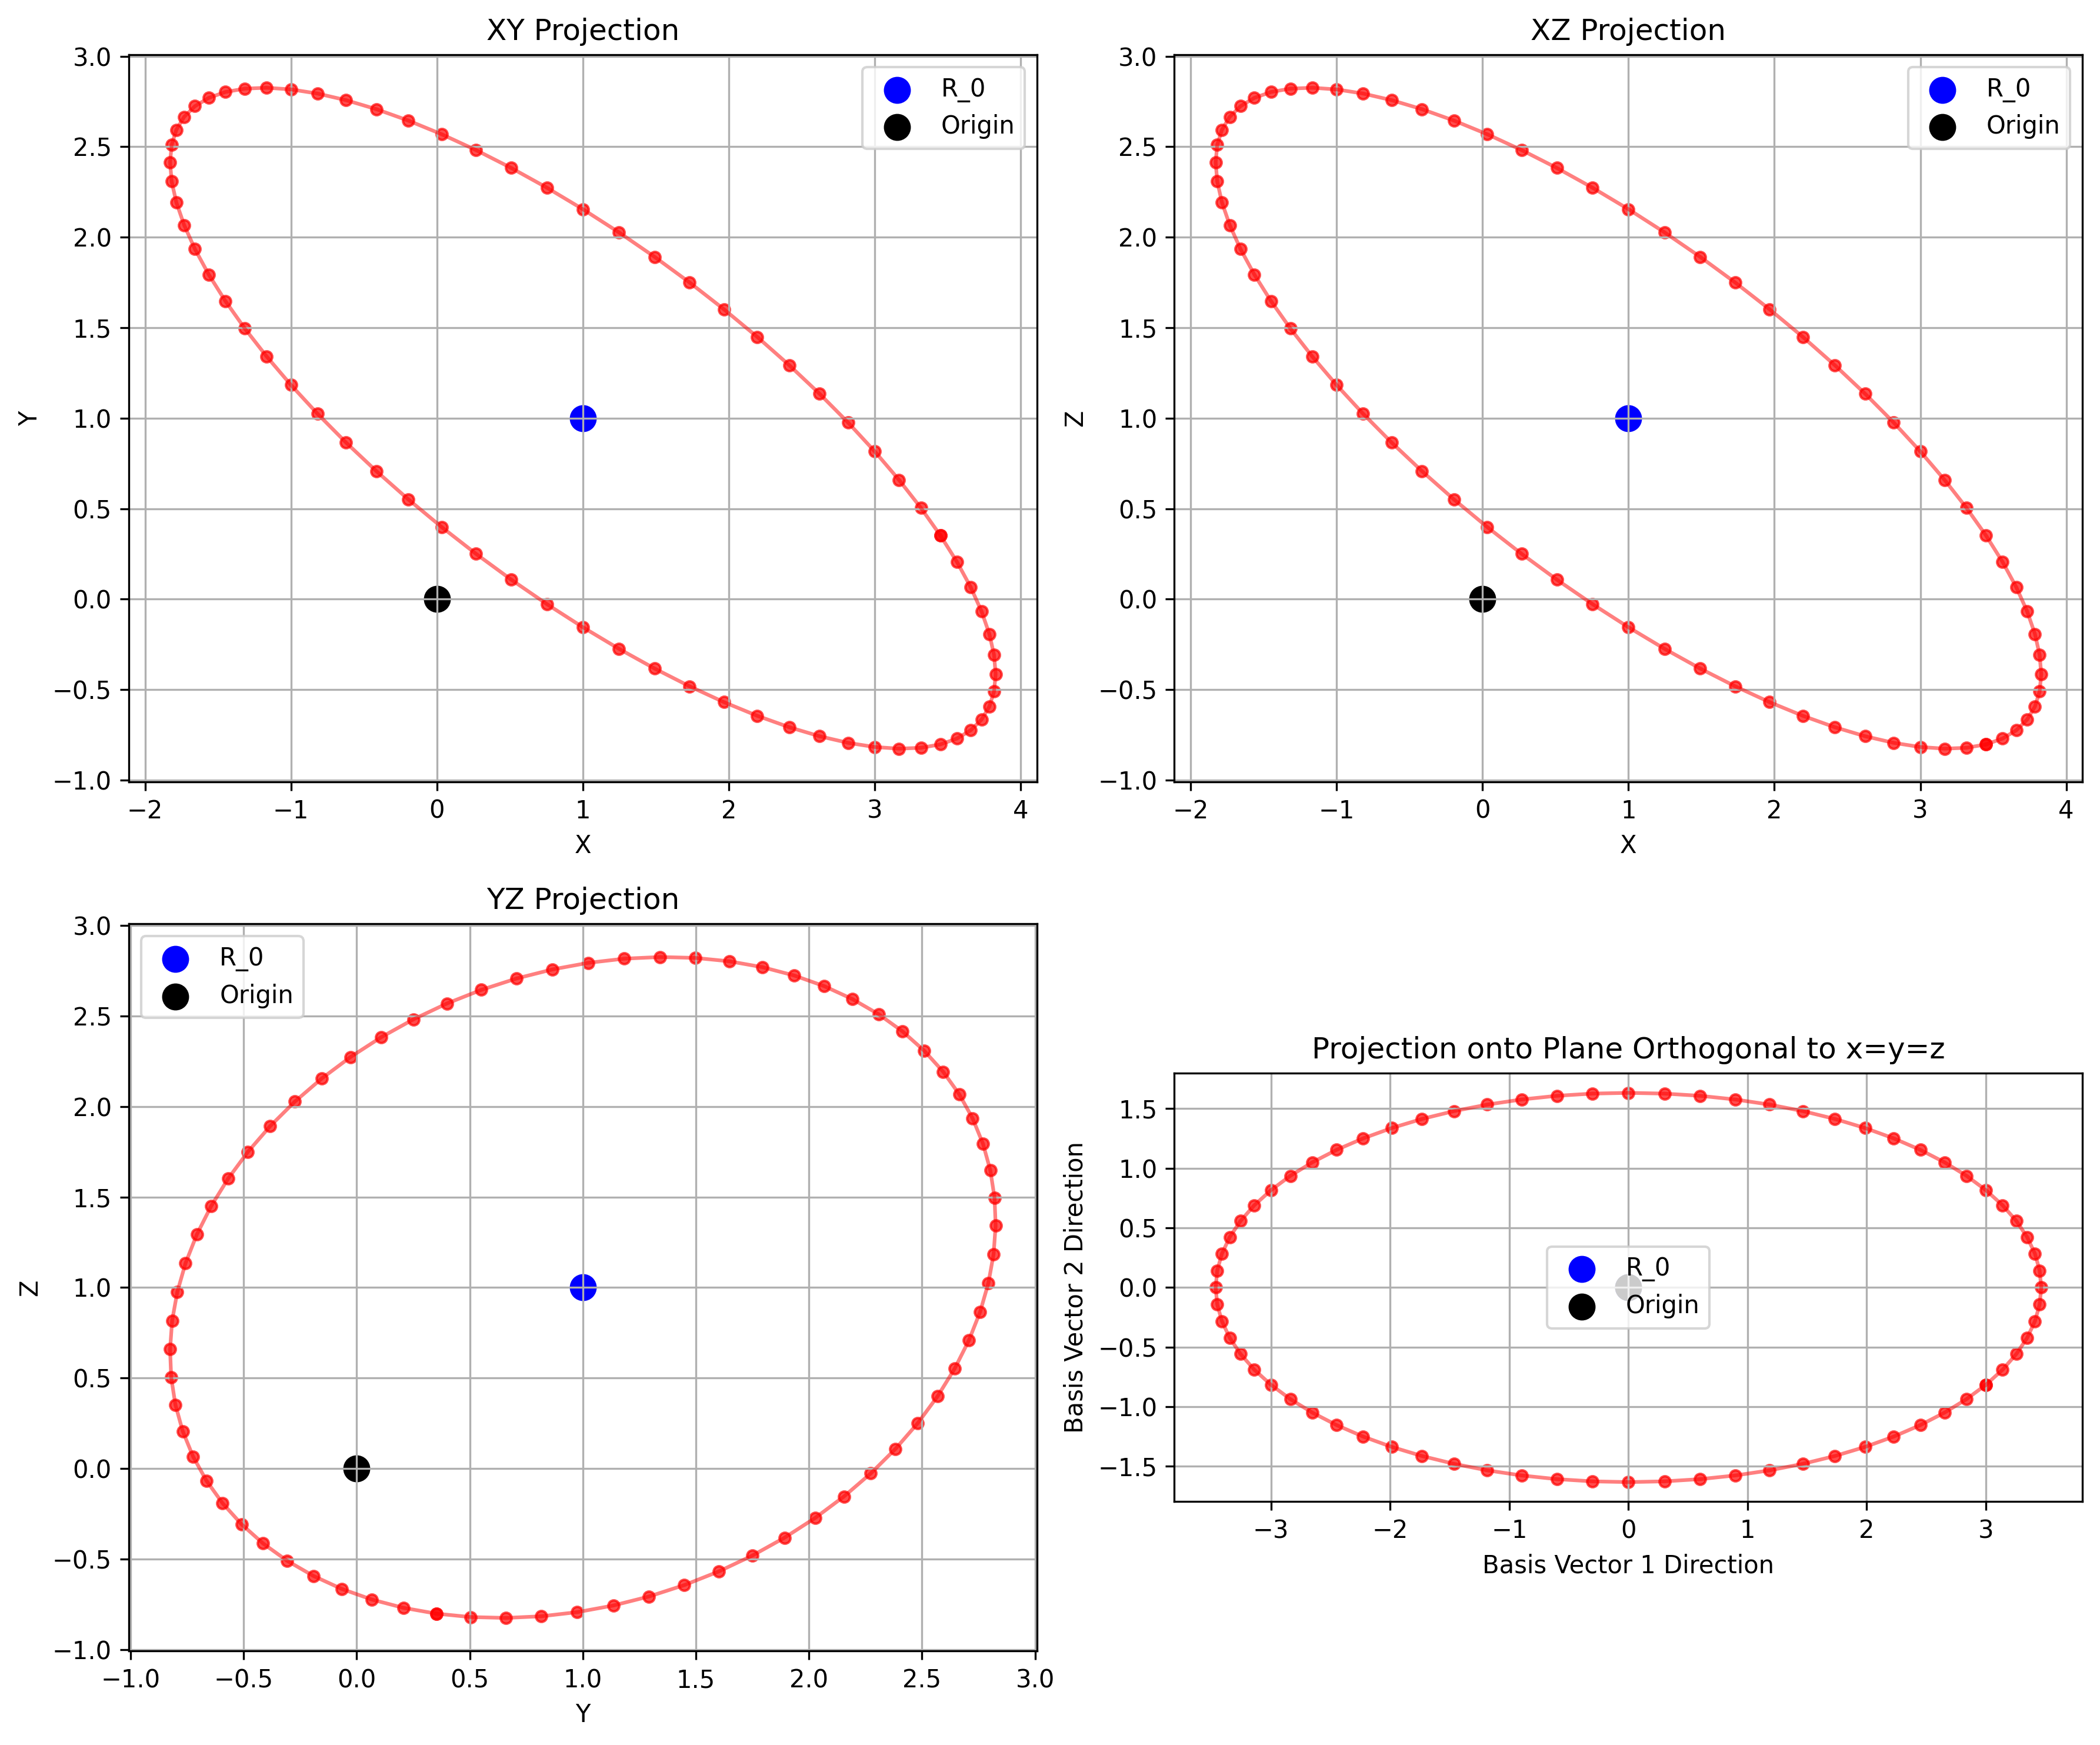
\includegraphics[width=0.8\textwidth]{figures/orthogonality_test/orthogonal_circle_projections.png}
    \caption{Projections of the circle onto different planes, including the plane orthogonal to the x=y=z line (bottom right)}
    \label{fig:orthogonal_circle_projections}
\end{figure}

\subsubsection{Orthogonality Verification Results}

The tests verified orthogonality by calculating the dot product between the displacement vector (R - R\_0) and the normalized (1,1,1) direction:

\begin{itemize}
    \item Maximum dot product across all points: 5.55e-16
    \item Average dot product: 1.39e-16
\end{itemize}

These values are effectively zero (within floating-point precision), confirming that all generated vectors are orthogonal to the x=y=z line.

\subsection{Parameter Effects in Basis Vector Formulation}

The basis vector formulation uses two key parameters to control the generated vectors: the distance parameter $d$ and the angle parameter $\theta$. These parameters interact with the origin vector to produce a wide variety of vector configurations while maintaining orthogonality to the x=y=z line.

\subsubsection{Distance Parameter}

In the basis vector formulation, the distance parameter $d$ appears as a scaling factor in the formula:

\begin{align}
\vec{R} = \vec{R}_0 + d \cdot \cos(\theta) \cdot \sqrt{\frac{2}{3}} \cdot \vec{b}_1 + d \cdot \frac{\cos(\theta)/\sqrt{3} + \sin(\theta)}{\sqrt{2}} \cdot \vec{b}_1 + d \cdot \frac{\sin(\theta) - \cos(\theta)/\sqrt{3}}{\sqrt{2}} \cdot \vec{b}_2 \cdot \sqrt{2}
\end{align}

where $\vec{b}_1 = [1, -1/2, -1/2]$ and $\vec{b}_2 = [0, -1/2, 1/2]$ are the basis vectors orthogonal to the (1,1,1) direction.

This parameter controls the overall scale of the vector displacement from the origin. Larger values of $d$ result in vectors that extend further from the origin, while smaller values produce vectors closer to the origin. The distance parameter affects all components of the vector equally, preserving the directional properties determined by $\theta$ and the orthogonality to the x=y=z line.

\subsubsection{Angle Parameter}

The angle parameter $\theta$ appears in both sine and cosine terms in the basis vector formula. This parameter controls the orientation of the generated vector within the plane orthogonal to the x=y=z line. As $\theta$ varies, the vector traces a circle in the plane orthogonal to the x=y=z line.

\subsubsection{Multiple Perfect Circles with Different Distances}

To illustrate the effect of the distance parameter $d$, we can generate multiple perfect circles with different distance values while keeping the same origin and angle range. Figure \ref{fig:perfect_circle_distance_range} shows perfect orthogonal circles with distances ranging from 0.5 to 3.0 in 0.5 increments, all centered at the origin [0.0, 0.0, 0.0].

\begin{figure}[H]
    \centering
    \includegraphics[width=0.8\textwidth]{../../../perfect_circle_distance_range.png}
    \caption{3D visualization of perfect orthogonal circles with different distance values (d = 0.5 to 3.0)}
    \label{fig:perfect_circle_distance_range}
\end{figure}

\begin{figure}[H]
    \centering
    \includegraphics[width=0.8\textwidth]{../../../perfect_circle_distance_range_projections.png}
    \caption{Projections of the perfect orthogonal circles with different distance values onto different planes}
    \label{fig:perfect_circle_distance_range_projections}
\end{figure}

These figures clearly demonstrate how the distance parameter $d$ controls the radius of the circle in the plane orthogonal to the x=y=z line. All points on each circle remain perfectly orthogonal to the x=y=z line, regardless of the distance value. This property makes the perfect orthogonal circle generation method particularly useful for applications requiring precise control over both orthogonality and distance from the origin.

\subsubsection{Enhanced Visualization Features}

The visualizations incorporate several enhancements for improved clarity and spatial understanding:

\begin{itemize}
    \item \textbf{Color-coded Axes}: The X (red), Y (green), and Z (blue) axes are color-coded for easy identification.
    \item \textbf{Coordinate Labels}: Integer coordinate values are displayed along each axis, color-matched to the axis color.
    \item \textbf{Tick Marks}: Small tick marks are added along each axis for better spatial reference.
    \item \textbf{Data-driven Scaling}: The axis limits are dynamically adjusted based on the actual data points, making the circles more prominent in the visualization.
    \item \textbf{Equal Aspect Ratio}: The 3D plots maintain an equal aspect ratio for accurate spatial representation.
    \item \textbf{Buffer Zones}: Small buffer zones are added around the data points for better visibility.
\end{itemize}

These visualization enhancements significantly improve the clarity of the 3D representations, making it easier to understand the spatial relationships between the circles and their orthogonality to the x=y=z line.

The angle parameter works by controlling the linear combination of the two basis vectors $\vec{b}_1 = [1, -1/2, -1/2]$ and $\vec{b}_2 = [0, -1/2, 1/2]$, which span the plane orthogonal to the (1,1,1) direction. As $\theta$ varies, the vector traces a circular path in this orthogonal plane while maintaining a constant distance from the origin (for fixed $d$). The sine and cosine terms determine the specific linear combination, ensuring that the resulting vector always remains orthogonal to the x=y=z line.

When $\theta$ is varied from 0 to $2\pi$ with a fixed distance parameter, the resulting vectors form a perfect circle in the plane orthogonal to the x=y=z line, as demonstrated in the orthogonality test results. This is fundamentally different from a traditional circle in the XY plane, which is not generally orthogonal to the (1,1,1) direction.

The orthogonality to the x=y=z line is maintained for all values of $\theta$, as verified by the dot product calculations in the orthogonality tests.

\subsubsection{Flexible Parameter Support}

The perfect orthogonal circle generation method supports flexible parameters for customization:

\begin{itemize}
    \item \textbf{Arbitrary Origin}: The circle can be generated around any origin point $\vec{R}_0$, not just the coordinate system origin.
    \item \textbf{Variable Distance}: The distance parameter $d$ can be set to any positive value, controlling the radius of the circle.
    \item \textbf{Theta Range}: The circle can be generated as a complete circle or as a segment by specifying start\_theta and end\_theta parameters.
\end{itemize}

\subsubsection{Parameter Verification Results}

Comprehensive testing with different parameter values confirms the robustness of the implementation:

\begin{table}[H]
    \centering
    \begin{tabular}{|c|c|c|c|}
        \hline
        \textbf{Distance ($d$)} & \textbf{Mean Distance} & \textbf{Std. Dev.} & \textbf{Max Dot Product} \\ \hline
        0.5 & 0.5 & 1.18e-16 & 1.94e-16 \\ \hline
        1.0 & 1.0 & 1.35e-16 & 1.67e-16 \\ \hline
        2.0 & 2.0 & 2.16e-16 & 3.33e-16 \\ \hline
        3.0 & 3.0 & 3.70e-16 & 3.33e-16 \\ \hline
    \end{tabular}
    \caption{Verification results for different distance values}
    \label{tab:distance_verification}
\end{table}

\begin{table}[H]
    \centering
    \begin{tabular}{|c|c|c|c|c|}
        \hline
        \textbf{Theta Range} & \textbf{Mean Distance} & \textbf{Std. Dev.} & \textbf{Max Dot Product} & \textbf{Points} \\ \hline
        $(0, \pi/2)$ & 2.0 & 1.89e-16 & 3.33e-16 & 18 \\ \hline
        $(0, \pi)$ & 2.0 & 2.09e-16 & 3.33e-16 & 18 \\ \hline
        $(\pi/4, 3\pi/4)$ & 2.0 & 2.22e-16 & 4.44e-16 & 18 \\ \hline
        $(0, 2\pi)$ & 2.0 & 2.56e-16 & 3.33e-16 & 18 \\ \hline
    \end{tabular}
    \caption{Verification results for different theta ranges}
    \label{tab:theta_verification}
\end{table}

\begin{figure}[H]
    \centering
    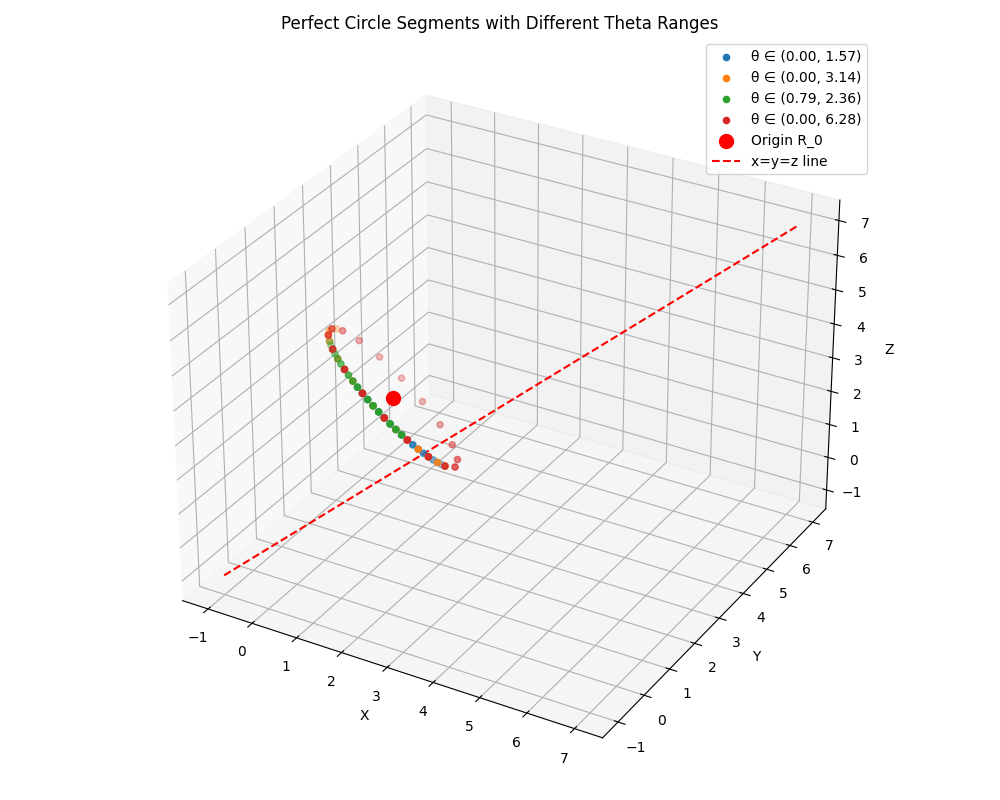
\includegraphics[width=0.8\textwidth]{../../../perfect_circle_tests.png}
    \caption{3D visualization of perfect circles with different distance values and theta ranges}
    \label{fig:perfect_circle_tests}
\end{figure}

These results confirm that the perfect orthogonal circle implementation maintains exact distance from the origin and perfect orthogonality to the (1,1,1) direction across all parameter variations. The standard deviation of distances is effectively zero (within floating-point precision), and the maximum dot product with the (1,1,1) direction is also effectively zero.


\subsection{Summary of Results}

The example results demonstrate that the Generalized Orthogonal Vectors Generator and Visualizer successfully generates and visualizes orthogonal vectors for various configurations. The vectors are confirmed to be orthogonal by calculating their dot products, which are all zero (within numerical precision).

The visualizations show the vectors in both 3D and 2D projections, providing different perspectives on their spatial relationships. The enhanced visualization features, including color-coded axes, coordinate labels, and data-driven scaling, significantly improve the clarity of the representations and make it easier to understand the spatial relationships between the vectors.

The effects of the distance parameter, angle parameter, and origin on the vector system are clearly demonstrated through the various examples, with the improved visualizations making these relationships more apparent.

\newpage
\section{Conclusion}

The Generalized Orthogonal Vectors Generator and Visualizer package provides a comprehensive solution for generating and visualizing vectors orthogonal to the x=y=z line in three-dimensional space. This document has described the mathematical formulation using basis vectors, implementation details, API reference, usage examples, visualization techniques, configuration system, command-line interface, and example results of the package, with a focus on ensuring orthogonality to the (1,1,1) direction.

\subsection{Summary of Features}

The package offers the following key features:

\begin{itemize}
    \item \textbf{Mathematical Rigor}: The package is based on a mathematically proven formulation using basis vectors [1, -1/2, -1/2] and [0, -1/2, 1/2] for generating vectors orthogonal to the x=y=z line, ensuring the correctness of the results as verified by comprehensive testing.
    
    \item \textbf{Perfect Orthogonal Circle Generation}: The package includes a specialized implementation for generating perfect circles in the plane orthogonal to the x=y=z line, with verification that all points are exactly at the specified distance from the origin and perfectly orthogonal to the (1,1,1) direction.
    
    \item \textbf{Enhanced Visualization}: The package provides advanced visualization features including color-coded axes (X: red, Y: green, Z: blue), coordinate labels along each axis, small tick marks for better spatial reference, and data-driven axis scaling that focuses on the actual data points.
    
    \item \textbf{Modular Architecture}: The package is organized into separate modules for vector calculations, visualization, and configuration management, making it easy to maintain, extend, and reuse.
    
    \item \textbf{Configurability}: All aspects of vector generation and visualization can be configured through a unified configuration system, allowing for customization without modifying the code.
    
    \item \textbf{Command-line Interface}: The package provides a comprehensive command-line interface that allows users to generate and visualize orthogonal vectors without writing Python code.
    
    \item \textbf{Configuration File Support}: Configurations can be saved to and loaded from JSON files, making it easy to reuse configurations across different runs.
    
    \item \textbf{Multiple Visualization Options}: The package supports both 3D visualization and various 2D projections, providing different perspectives on the vectors.
    
    \item \textbf{Plot Saving}: Plots can be saved to files instead of being displayed interactively, allowing for the creation of visualizations for documentation or presentations.
    
    \item \textbf{Python Package}: The package can be used as a Python package, allowing for integration into other projects.
\end{itemize}

\subsection{Potential Applications}

The Generalized Orthogonal Vectors Generator and Visualizer package can be used in various applications, including:

\begin{itemize}
    \item \textbf{Educational Tools}: The package can be used as an educational tool for teaching concepts related to vectors, orthogonality, and three-dimensional geometry.
    
    \item \textbf{Scientific Visualization}: The package can be used for visualizing orthogonal vectors in scientific applications, such as physics simulations or computational geometry.
    
    \item \textbf{Computer Graphics}: The package can be used in computer graphics applications that require orthogonal coordinate systems, such as camera positioning or object orientation.
    
    \item \textbf{Robotics}: The package can be used in robotics applications that require orthogonal coordinate systems, such as robot arm positioning or sensor orientation.
\end{itemize}

\subsection{Future Work}

The Generalized Orthogonal Vectors Generator and Visualizer package can be extended in various ways, including:

\begin{itemize}
    \item \textbf{Additional Visualization Options}: The package could be extended to support additional visualization options, such as interactive 3D visualization or animation of vector rotation.
    
    \item \textbf{Further Visualization Enhancements}: Building on the recent improvements in axis representation and scaling, future work could include more advanced visualization features such as customizable axis appearance, additional projection methods, and interactive axis controls.
    
    \item \textbf{More Advanced Configuration Management}: The configuration management system could be extended to support more advanced features, such as configuration validation or configuration inheritance.
    
    \item \textbf{Integration with Other Packages}: The package could be integrated with other Python packages for scientific computing or visualization, such as SciPy or Plotly.
    
    \item \textbf{Web Interface}: The package could be extended to provide a web interface for generating and visualizing orthogonal vectors, making it accessible to users without Python knowledge.
    
    \item \textbf{Performance Optimization}: The package could be optimized for performance, especially for applications that require generating and visualizing a large number of vectors.
    
    \item \textbf{Unit Tests}: The package could be extended with comprehensive unit tests to ensure the correctness of the implementation.
    
    \item \textbf{Documentation Improvements}: The documentation could be improved with more examples, tutorials, and explanations of the mathematical concepts.
\end{itemize}

\subsection{Conclusion}

The Generalized Orthogonal Vectors Generator and Visualizer package provides a powerful and flexible tool for generating and visualizing vectors orthogonal to the x=y=z line in three-dimensional space. Its basis vector approach ensures mathematical precision in maintaining orthogonality to the (1,1,1) direction, as demonstrated by the test results showing dot products effectively at zero. The implementation of perfect orthogonal circle generation further demonstrates the mathematical precision of the approach, creating circles where all points are exactly at the specified distance from the origin and perfectly orthogonal to the (1,1,1) direction. The package's modular architecture, configurability, and comprehensive features make it suitable for a wide range of applications, from educational tools to scientific visualization. The package is designed to be easy to use, both as a command-line tool and as a Python package, making it accessible to users with different levels of programming experience.


\appendix

\newpage
\section{Source Code}

This appendix contains the complete source code for the Orthogonal Vector Visualization System package.

\subsection{Example Scripts}

\subsubsection{perfect\_circle\_distance\_range.py}

\begin{lstlisting}[language=Python]
#!/usr/bin/env python3
"""
Generate perfect orthogonal circles with different distance values.
This script creates circles in the plane orthogonal to the (1,1,1) direction
with distances ranging from 0.5 to 3.0 in 0.5 increments.
"""

import numpy as np
import matplotlib.pyplot as plt
from mpl_toolkits.mplot3d import Axes3D
import os
import sys

# Add the generalized directory to the path
sys.path.append(os.path.join(os.path.dirname(__file__), 'generalized'))
from vector_utils import create_perfect_orthogonal_circle

# Set up the figure
fig = plt.figure(figsize=(12, 10))
ax = fig.add_subplot(111, projection='3d')

# Define the origin
R_0 = np.array([0.0, 0.0, 0.0])

# Define the range of distances
distances = np.arange(0.5, 3.5, 0.5)

# Define the theta range (full circle)
theta_start = 0
theta_end = 2 * np.pi
num_points = 73  # 5-degree increments

# Generate and plot circles for each distance
colors = plt.cm.viridis(np.linspace(0, 1, len(distances)))

# Store all circle points for scaling calculations
all_circles_points = []

for i, d in enumerate(distances):
    # Generate the circle
    vectors = create_perfect_orthogonal_circle(
        R_0=R_0,
        d=d,
        start_theta=theta_start,
        end_theta=theta_end,
        num_points=num_points
    )
    
    # Store points for scaling calculations
    all_circles_points.append(vectors)
    
    # Plot the circle
    ax.scatter(vectors[:, 0], vectors[:, 1], vectors[:, 2], 
               color=colors[i], label=f'd = {d}')
    
    # We'll keep the circles without the connecting lines to make the visualization cleaner

# Plot the origin
ax.scatter(R_0[0], R_0[1], R_0[2], color='red', s=100, marker='o', label='Origin R_0')

# Add axis lines with higher visibility and labels
# Adjust max_val to be closer to the actual data for better visualization
max_val = max(np.max(np.abs(distances)) * 1.5, 3.5)

# X-axis - red with label and coordinate markers
ax.plot([-max_val, max_val], [0, 0], [0, 0], 'r-', alpha=0.6, linewidth=1.0)
ax.text(max_val*1.1, 0, 0, 'X', color='red', fontsize=12)

# Add coordinate markers along X-axis
for i in range(-int(max_val), int(max_val)+1):
    if i != 0 and i % 1 == 0:  # Only show integer values, skip zero
        ax.text(i, 0, 0, f'{i}', color='red', fontsize=8, ha='center', va='bottom')
        # Add small tick marks
        ax.plot([i, i], [0, -0.05], [0, 0], 'r-', alpha=0.4, linewidth=0.5)

# Y-axis - green with label and coordinate markers
ax.plot([0, 0], [-max_val, max_val], [0, 0], 'g-', alpha=0.6, linewidth=1.0)
ax.text(0, max_val*1.1, 0, 'Y', color='green', fontsize=12)

# Add coordinate markers along Y-axis
for i in range(-int(max_val), int(max_val)+1):
    if i != 0 and i % 1 == 0:  # Only show integer values, skip zero
        ax.text(0, i, 0, f'{i}', color='green', fontsize=8, ha='right', va='center')
        # Add small tick marks
        ax.plot([0, -0.05], [i, i], [0, 0], 'g-', alpha=0.4, linewidth=0.5)

# Z-axis - blue with label and coordinate markers
ax.plot([0, 0], [0, 0], [-max_val, max_val], 'b-', alpha=0.6, linewidth=1.0)
ax.text(0, 0, max_val*1.1, 'Z', color='blue', fontsize=12)

# Add coordinate markers along Z-axis
for i in range(-int(max_val), int(max_val)+1):
    if i != 0 and i % 1 == 0:  # Only show integer values, skip zero
        ax.text(0, 0, i, f'{i}', color='blue', fontsize=8, ha='right', va='center')
        # Add small tick marks
        ax.plot([0, -0.05], [0, 0], [i, i], 'b-', alpha=0.4, linewidth=0.5)

# Plot the x=y=z line
line = np.array([[-1, -1, -1], [7, 7, 7]])
ax.plot(line[:, 0], line[:, 1], line[:, 2], 'r--', label='x=y=z line')

# Set labels and title
ax.set_xlabel('X')
ax.set_ylabel('Y')
ax.set_zlabel('Z')
ax.set_title('Perfect Orthogonal Circles with Different Distances', fontsize=14)

# Calculate data range for better scaling
data_min = min([np.min(vectors) for vectors in all_circles_points])
data_max = max([np.max(vectors) for vectors in all_circles_points])
data_max = max(abs(data_min), abs(data_max))

# Add a small buffer for better visualization
buffer = data_max * 0.1

# Set axis limits
ax.set_xlim([-data_max-buffer, data_max+buffer])
ax.set_ylim([-data_max-buffer, data_max+buffer])
ax.set_zlim([-data_max-buffer, data_max+buffer])

# Set equal aspect ratio for better 3D visualization
ax.set_box_aspect([1, 1, 1])

# Add a legend
ax.legend()

# Save the figure
plt.savefig('perfect_circle_distance_range.png', dpi=300, bbox_inches='tight')

# Create a second figure with 2D projections
fig2, axs = plt.subplots(2, 2, figsize=(14, 12))
axs = axs.flatten()

# XY Projection
for i, d in enumerate(distances):
    vectors = create_perfect_orthogonal_circle(
        R_0=R_0,
        d=d,
        start_theta=theta_start,
        end_theta=theta_end,
        num_points=num_points
    )
    axs[0].scatter(vectors[:, 0], vectors[:, 1], color=colors[i], label=f'd = {d}')

axs[0].scatter(R_0[0], R_0[1], color='red', s=100, marker='o')
axs[0].set_xlabel('X')
axs[0].set_ylabel('Y')
axs[0].set_title('XY Projection')
axs[0].grid(True)
axs[0].set_aspect('equal')

# XZ Projection
for i, d in enumerate(distances):
    vectors = create_perfect_orthogonal_circle(
        R_0=R_0,
        d=d,
        start_theta=theta_start,
        end_theta=theta_end,
        num_points=num_points
    )
    axs[1].scatter(vectors[:, 0], vectors[:, 2], color=colors[i])

axs[1].scatter(R_0[0], R_0[2], color='red', s=100, marker='o')
axs[1].set_xlabel('X')
axs[1].set_ylabel('Z')
axs[1].set_title('XZ Projection')
axs[1].grid(True)
axs[1].set_aspect('equal')

# YZ Projection
for i, d in enumerate(distances):
    vectors = create_perfect_orthogonal_circle(
        R_0=R_0,
        d=d,
        start_theta=theta_start,
        end_theta=theta_end,
        num_points=num_points
    )
    axs[2].scatter(vectors[:, 1], vectors[:, 2], color=colors[i])

axs[2].scatter(R_0[1], R_0[2], color='red', s=100, marker='o')
axs[2].set_xlabel('Y')
axs[2].set_ylabel('Z')
axs[2].set_title('YZ Projection')
axs[2].grid(True)
axs[2].set_aspect('equal')

# Orthogonal Plane Projection
# Define the basis vectors for the orthogonal plane
basis1 = np.array([1, -1/2, -1/2])
basis2 = np.array([0, -1/2, 1/2])

# Normalize the basis vectors
basis1 = basis1 / np.linalg.norm(basis1)
basis2 = basis2 / np.linalg.norm(basis2)

for i, d in enumerate(distances):
    vectors = create_perfect_orthogonal_circle(
        R_0=R_0,
        d=d,
        start_theta=theta_start,
        end_theta=theta_end,
        num_points=num_points
    )
    
    # Project onto the orthogonal plane
    projected_points = []
    for v in vectors:
        # Vector from R_0 to the point
        v_rel = v - R_0
        
        # Project onto the basis vectors
        x_proj = np.dot(v_rel, basis1)
        y_proj = np.dot(v_rel, basis2)
        
        projected_points.append([x_proj, y_proj])
    
    projected_points = np.array(projected_points)
    axs[3].scatter(projected_points[:, 0], projected_points[:, 1], color=colors[i])

axs[3].scatter(0, 0, color='red', s=100, marker='o')
axs[3].set_xlabel('Basis Vector 1')
axs[3].set_ylabel('Basis Vector 2')
axs[3].set_title('Projection onto Plane Orthogonal to x=y=z')
axs[3].grid(True)
axs[3].set_aspect('equal')

# Add a legend to the first subplot only to avoid clutter
axs[0].legend(loc='upper right')

# Adjust layout and save
plt.tight_layout()
plt.savefig('perfect_circle_distance_range_projections.png', dpi=300, bbox_inches='tight')

plt.show()
\end{lstlisting}

\subsubsection{perfect\_orthogonal\_circle.py}

\begin{lstlisting}[language=Python]
#!/usr/bin/env python3
"""
Generate and visualize a perfect circle in the plane orthogonal to the x=y=z line.
This script uses R_0 = (0,0,0), d=1, and theta ranging from 0 to 360 degrees in 5-degree steps.
"""

import numpy as np
import matplotlib.pyplot as plt
from mpl_toolkits.mplot3d import Axes3D
import os

def generate_perfect_orthogonal_circle(d=1.0, num_points=73):
    """
    Generate a perfect circle in the plane orthogonal to the x=y=z line.
    
    Parameters:
    d (float): Distance parameter, default is 1.0
    num_points (int): Number of points to generate, default is 73 (5-degree steps)
    
    Returns:
    numpy.ndarray: Array of points forming the circle
    """
    # Set R_0 to (0,0,0)
    R_0 = np.array([0, 0, 0])
    
    # Define the basis vectors orthogonal to the (1,1,1) direction
    basis1 = np.array([1, -1/2, -1/2])
    basis2 = np.array([0, -1/2, 1/2])
    
    # Normalize the basis vectors
    basis1 = basis1 / np.linalg.norm(basis1)
    basis2 = basis2 / np.linalg.norm(basis2)
    
    # Generate theta values from 0 to 2*np.pi
    thetas = np.linspace(0, 2*np.pi, num_points)
    
    # Generate points directly using the basis vectors to ensure a perfect circle
    points = []
    for theta in thetas:
        # Create a point at distance d from the origin in the plane spanned by basis1 and basis2
        point = R_0 + d * (np.cos(theta) * basis1 + np.sin(theta) * basis2)
        points.append(point)
    
    return np.array(points)

def visualize_perfect_orthogonal_circle(points):
    """
    Visualize the perfect circle in the plane orthogonal to the x=y=z line.
    
    Parameters:
    points (numpy.ndarray): Array of points forming the circle
    """
    # Create output directory if it doesn't exist
    output_dir = "perfect_circle_output"
    os.makedirs(output_dir, exist_ok=True)
    
    # 3D visualization
    fig = plt.figure(figsize=(10, 8))
    ax = fig.add_subplot(111, projection='3d')
    
    # Plot the circle points
    ax.scatter(points[:, 0], points[:, 1], points[:, 2], c='b', marker='o')
    
    # Plot the origin
    ax.scatter(0, 0, 0, c='r', marker='o', s=100)
    
    # Plot the x=y=z line
    line = np.array([[-1, -1, -1], [1, 1, 1]])
    ax.plot(line[:, 0], line[:, 1], line[:, 2], 'r--')
    
    # Set labels and title
    ax.set_xlabel('X')
    ax.set_ylabel('Y')
    ax.set_zlabel('Z')
    ax.set_title('Perfect Circle Orthogonal to x=y=z Line')
    
    # Save the figure
    plt.savefig(f"{output_dir}/perfect_circle_3d.png")
    
    # Create a figure for projections
    fig, axs = plt.subplots(2, 2, figsize=(12, 10))
    
    # XY projection
    axs[0, 0].scatter(points[:, 0], points[:, 1], c='b', marker='o')
    axs[0, 0].scatter(0, 0, c='r', marker='o', s=100)
    axs[0, 0].set_xlabel('X')
    axs[0, 0].set_ylabel('Y')
    axs[0, 0].set_title('XY Projection')
    axs[0, 0].grid(True)
    axs[0, 0].axis('equal')
    
    # XZ projection
    axs[0, 1].scatter(points[:, 0], points[:, 2], c='b', marker='o')
    axs[0, 1].scatter(0, 0, c='r', marker='o', s=100)
    axs[0, 1].set_xlabel('X')
    axs[0, 1].set_ylabel('Z')
    axs[0, 1].set_title('XZ Projection')
    axs[0, 1].grid(True)
    axs[0, 1].axis('equal')
    
    # YZ projection
    axs[1, 0].scatter(points[:, 1], points[:, 2], c='b', marker='o')
    axs[1, 0].scatter(0, 0, c='r', marker='o', s=100)
    axs[1, 0].set_xlabel('Y')
    axs[1, 0].set_ylabel('Z')
    axs[1, 0].set_title('YZ Projection')
    axs[1, 0].grid(True)
    axs[1, 0].axis('equal')
    
    # Project onto the plane orthogonal to (1,1,1)
    # Use the basis vectors to create 2D coordinates in the orthogonal plane
    basis1 = np.array([1, -1/2, -1/2])
    basis2 = np.array([0, -1/2, 1/2])
    
    # Normalize the basis vectors
    basis1 = basis1 / np.linalg.norm(basis1)
    basis2 = basis2 / np.linalg.norm(basis2)
    
    # Project each point onto the basis vectors
    proj_x = np.array([np.dot(p, basis1) for p in points])
    proj_y = np.array([np.dot(p, basis2) for p in points])
    
    # Plot the projection onto the orthogonal plane
    axs[1, 1].scatter(proj_x, proj_y, c='b', marker='o')
    axs[1, 1].scatter(0, 0, c='r', marker='o', s=100)
    axs[1, 1].set_xlabel('Basis Vector 1')
    axs[1, 1].set_ylabel('Basis Vector 2')
    axs[1, 1].set_title('Projection onto Orthogonal Plane')
    axs[1, 1].grid(True)
    axs[1, 1].axis('equal')
    
    plt.tight_layout()
    plt.savefig(f"{output_dir}/perfect_circle_projections.png")
    
    # Create a separate figure for the orthogonal plane projection
    plt.figure(figsize=(8, 8))
    plt.scatter(proj_x, proj_y, c='b', marker='o')
    plt.scatter(0, 0, c='r', marker='o', s=100)
    plt.xlabel('Basis Vector 1')
    plt.ylabel('Basis Vector 2')
    plt.title('Projection onto Plane Orthogonal to x=y=z Line')
    plt.grid(True)
    plt.axis('equal')
    plt.tight_layout()
    plt.savefig(f"{output_dir}/perfect_circle_orthogonal_plane.png")

def verify_circle_properties(points):
    """
    Verify that the generated points form a perfect circle.
    
    Parameters:
    points (numpy.ndarray): Array of points forming the circle
    
    Returns:
    dict: Dictionary containing verification results
    """
    # Calculate distances from the origin
    distances = np.linalg.norm(points, axis=1)
    
    # Calculate dot products with the (1,1,1) direction
    unit_111 = np.array([1, 1, 1]) / np.sqrt(3)
    dot_products = np.abs(np.array([np.dot(p, unit_111) for p in points]))
    
    # Calculate results
    results = {
        'mean_distance': np.mean(distances),
        'std_distance': np.std(distances),
        'min_distance': np.min(distances),
        'max_distance': np.max(distances),
        'distance_ratio': np.max(distances) / np.min(distances),
        'max_dot_product': np.max(dot_products),
        'mean_dot_product': np.mean(dot_products)
    }
    
    # Print the results
    print("\nVerification Results:")
    print(f"Mean distance from origin: {results['mean_distance']:.10f}")
    print(f"Standard deviation of distances: {results['std_distance']:.10e}")
    print(f"Min/max distance ratio: {results['distance_ratio']:.10f}")
    print(f"Maximum dot product with (1,1,1): {results['max_dot_product']:.10e}")
    print(f"Average dot product with (1,1,1): {results['mean_dot_product']:.10e}")
    
    return results

def main():
    """
    Main function to generate and visualize the perfect orthogonal circle.
    """
    print("Generating perfect orthogonal circle...")
    points = generate_perfect_orthogonal_circle(d=1.0, num_points=73)
    
    print("Verifying circle properties...")
    verify_circle_properties(points)
    
    print("Visualizing perfect orthogonal circle...")
    visualize_perfect_orthogonal_circle(points)
    
    print("Done!")

if __name__ == "__main__":
    main()
\end{lstlisting}

\subsubsection{test\_perfect\_circle\_ranges.py}

\begin{lstlisting}[language=Python]
#!/usr/bin/env python3
import numpy as np
from generalized.vector_utils import create_orthogonal_vectors
import matplotlib.pyplot as plt
from mpl_toolkits.mplot3d import Axes3D

def test_perfect_circle_ranges():
    """
    Test the perfect circle generation with different d values and theta ranges
    """
    # Test with different parameters
    R_0 = np.array([1, 2, 3])  # Origin
    
    # Test 1: Different d values
    print("Test 1: Different d values")
    d_values = [0.5, 1.0, 2.0, 3.0]
    num_points = 36
    
    # Create figure for 3D visualization
    fig = plt.figure(figsize=(10, 8))
    ax = fig.add_subplot(111, projection='3d')
    
    for d in d_values:
        # Generate vectors
        vectors = create_orthogonal_vectors(R_0, d, num_points, perfect=True)
        
        # Check properties
        distances = np.array([np.linalg.norm(v - R_0) for v in vectors])
        unit_111 = np.array([1, 1, 1]) / np.sqrt(3)
        dot_products = np.array([np.abs(np.dot(v - R_0, unit_111)) for v in vectors])
        
        # Print results
        print(f"\nCircle with d = {d}:")
        print(f"  Mean distance from origin: {np.mean(distances)}")
        print(f"  Standard deviation of distances: {np.std(distances)}")
        print(f"  Maximum dot product with (1,1,1): {np.max(dot_products)}")
        
        # Plot the circle
        ax.scatter(vectors[:, 0], vectors[:, 1], vectors[:, 2], label=f'd = {d}')
    
    # Plot the origin
    ax.scatter(R_0[0], R_0[1], R_0[2], color='red', s=100, marker='o', label='Origin R_0')
    
    # Plot the x=y=z line
    line = np.array([[-1, -1, -1], [7, 7, 7]])
    ax.plot(line[:, 0], line[:, 1], line[:, 2], 'r--', label='x=y=z line')
    
    ax.set_xlabel('X')
    ax.set_ylabel('Y')
    ax.set_zlabel('Z')
    ax.set_title('Perfect Circles with Different d Values')
    ax.legend()
    
    # Test 2: Different theta ranges
    print("\nTest 2: Different theta ranges")
    d = 2.0
    num_points = 18
    
    theta_ranges = [
        (0, np.pi/2),          # Quarter circle
        (0, np.pi),            # Half circle
        (np.pi/4, 3*np.pi/4),  # Middle segment
        (0, 2*np.pi)           # Full circle
    ]
    
    # Create figure for 3D visualization
    fig2 = plt.figure(figsize=(10, 8))
    ax2 = fig2.add_subplot(111, projection='3d')
    
    for start_theta, end_theta in theta_ranges:
        # Generate vectors
        vectors = create_orthogonal_vectors(R_0, d, num_points, perfect=True, 
                                          start_theta=start_theta, end_theta=end_theta)
        
        # Check properties
        distances = np.array([np.linalg.norm(v - R_0) for v in vectors])
        unit_111 = np.array([1, 1, 1]) / np.sqrt(3)
        dot_products = np.array([np.abs(np.dot(v - R_0, unit_111)) for v in vectors])
        
        # Print results
        range_desc = f"({start_theta:.2f}, {end_theta:.2f})"
        print(f"\nCircle segment with theta range {range_desc}:")
        print(f"  Mean distance from origin: {np.mean(distances)}")
        print(f"  Standard deviation of distances: {np.std(distances)}")
        print(f"  Maximum dot product with (1,1,1): {np.max(dot_products)}")
        print(f"  Number of points: {len(vectors)}")
        
        # Plot the circle segment
        label = f'theta in {range_desc}'
        ax2.scatter(vectors[:, 0], vectors[:, 1], vectors[:, 2], label=label)
    
    # Plot the origin
    ax2.scatter(R_0[0], R_0[1], R_0[2], color='red', s=100, marker='o', label='Origin R_0')
    
    # Plot the x=y=z line
    line = np.array([[-1, -1, -1], [7, 7, 7]])
    ax2.plot(line[:, 0], line[:, 1], line[:, 2], 'r--', label='x=y=z line')
    
    ax2.set_xlabel('X')
    ax2.set_ylabel('Y')
    ax2.set_zlabel('Z')
    ax2.set_title('Perfect Circle Segments with Different Theta Ranges')
    ax2.legend()
    
    plt.tight_layout()
    plt.savefig('perfect_circle_tests.png')
    plt.show()

if __name__ == "__main__":
    test_perfect_circle_ranges()
\end{lstlisting}

\subsubsection{example\_circle.py}

\begin{lstlisting}[language=Python]
#!/usr/bin/env python3
import numpy as np
import matplotlib.pyplot as plt
import math
import os
import sys

# Import from the generalized module
from vector_utils import create_orthogonal_vectors
from visualization import plot_multiple_vectors_3d, plot_multiple_vectors_2d, plot_multiple_vectors

def generate_circle_points():
    """
    Generate 72 points in a circle by varying theta from 0 to 360 degrees
    with a fixed distance d=0.1 from origin R_0=(0,0,0)
    
    Returns:
    list: List of tuples (d, theta, R) containing the parameters and vectors
    """
    # Set parameters
    R_0 = np.array([0, 0, 0])  # Origin
    d = 0.1                    # Fixed distance
    
    # Generate theta values from 0 to 360 degrees in steps of 5 degrees
    # Convert to radians for calculations
    theta_values = np.radians(np.arange(0, 361, 5))
    
    # Generate vectors for each theta value
    vectors = []
    for theta in theta_values:
        R = create_orthogonal_vectors(R_0, d, theta)
        vectors.append((d, theta, R))
        print(f"Generated point for theta={math.degrees(theta):.1f} deg: {R}")
    
    return R_0, vectors

def main():
    """
    Main function to generate and visualize circle points
    """
    print("Generating circle points...")
    R_0, vectors = generate_circle_points()
    
    print(f"\nGenerated {len(vectors)} points.")
    
    # Create plots directory if it doesn't exist
    output_dir = 'circle_plots'
    os.makedirs(output_dir, exist_ok=True)
    
    # Plot the points
    print("Creating plots...")
    plots = plot_multiple_vectors(
        R_0, 
        vectors,
        show_r0_plane=True,
        figsize_3d=(12, 10),
        figsize_2d=(10, 10),
        endpoints_only=True  # Only plot the endpoints
    )
    
    # Save the plots
    for name, (fig, _) in plots.items():
        filename = os.path.join(output_dir, f"circle_{name}.png")
        fig.savefig(filename)
        print(f"Saved plot to {filename}")
    
    # Show the plots
    plt.show()

if __name__ == "__main__":
    main()
\end{lstlisting}

\subsubsection{example\_circle\_xy.py}

\begin{lstlisting}[language=Python]
#!/usr/bin/env python3
import numpy as np
import matplotlib.pyplot as plt
import math
import os
import sys

def generate_circle_points_xy():
    """
    Generate 72 points in a circle in the XY plane by varying theta from 0 to 360 degrees
    with a fixed radius of 0.1 from origin (0,0,0)
    
    Returns:
    tuple: (R_0, vectors) where R_0 is the origin and vectors is a list of (d, theta, R) tuples
    """
    # Set parameters
    R_0 = np.array([0, 0, 0])  # Origin
    radius = 0.1               # Circle radius
    
    # Generate theta values from 0 to 360 degrees in steps of 5 degrees
    # Convert to radians for calculations
    theta_values = np.radians(np.arange(0, 361, 5))
    
    # Generate vectors for each theta value (traditional circle in XY plane)
    vectors = []
    for theta in theta_values:
        # Create a point on the circle in the XY plane
        x = radius * np.cos(theta)
        y = radius * np.sin(theta)
        z = 0  # Set z=0 for a flat circle in XY plane
        
        R = np.array([x, y, z])
        vectors.append((radius, theta, R))
        print(f"Generated point for theta={math.degrees(theta):.1f} deg: {R}")
    
    return R_0, vectors

def plot_multiple_vectors_3d(R_0, vectors, figsize=(12, 10), show_legend=True, endpoints_only=True):
    """
    Plot multiple vectors in 3D
    
    Parameters:
    R_0 (numpy.ndarray): The origin vector
    vectors (list): List of tuples (d, theta, R) containing the parameters and vectors
    figsize (tuple): Figure size (width, height) in inches
    show_legend (bool): Whether to show the legend
    endpoints_only (bool): If True, only plot the endpoints of vectors, not the arrows
    
    Returns:
    tuple: (fig, ax) matplotlib figure and axis objects
    """
    fig = plt.figure(figsize=figsize)
    ax = fig.add_subplot(111, projection='3d')
    
    # Plot the origin
    ax.scatter(R_0[0], R_0[1], R_0[2], color='black', s=100, label='R_0')
    
    # Get a colormap for the vectors
    cmap = plt.cm.get_cmap('viridis')
    num_vectors = len(vectors)
    
    # Extract all R vectors for axis scaling
    all_Rs = [R for _, _, R in vectors]
    
    # Plot the vectors
    for i, (d, theta, R) in enumerate(vectors):
        color = cmap(i / max(1, num_vectors - 1))
        label = f'R (theta={math.degrees(theta):.1f} deg)' if i % 10 == 0 else None
        
        # Plot only the endpoint
        ax.scatter(R[0], R[1], R[2], color=color, s=50, label=label)
    
    # Set labels and title
    ax.set_xlabel('X')
    ax.set_ylabel('Y')
    ax.set_zlabel('Z')
    ax.set_title('Circle Points in 3D (XY Plane)')
    
    # Set equal aspect ratio
    all_points = [R_0] + all_Rs
    max_range = np.array([
        np.max([p[0] for p in all_points]) - np.min([p[0] for p in all_points]),
        np.max([p[1] for p in all_points]) - np.min([p[1] for p in all_points]),
        np.max([p[2] for p in all_points]) - np.min([p[2] for p in all_points])
    ]).max() / 2.0
    
    mid_x = (np.max([p[0] for p in all_points]) + np.min([p[0] for p in all_points])) / 2
    mid_y = (np.max([p[1] for p in all_points]) + np.min([p[1] for p in all_points])) / 2
    mid_z = (np.max([p[2] for p in all_points]) + np.min([p[2] for p in all_points])) / 2
    
    ax.set_xlim(mid_x - max_range, mid_x + max_range)
    ax.set_ylim(mid_y - max_range, mid_y + max_range)
    ax.set_zlim(mid_z - max_range, mid_z + max_range)
    
    if show_legend:
        ax.legend()
    
    return fig, ax

def main():
    """
    Main function to generate and visualize circle points
    """
    print("Generating XY circle points...")
    R_0, vectors = generate_circle_points_xy()
    
    print(f"\nGenerated {len(vectors)} points.")
    
    # Create plots directory if it doesn't exist
    output_dir = 'circle_plots'
    os.makedirs(output_dir, exist_ok=True)
    
    # Plot the points in 3D
    print("Creating 3D plot...")
    fig_3d, _ = plot_multiple_vectors_3d(R_0, vectors, endpoints_only=True)
    
    # Save the 3D plot
    filename_3d = os.path.join(output_dir, "3d_xy_circle.png")
    fig_3d.savefig(filename_3d)
    print(f"Saved 3D plot to {filename_3d}")
    
    # Plot the points in 2D (XY plane)
    print("Creating 2D plot...")
    fig_2d = plt.figure(figsize=(10, 10))
    ax_2d = fig_2d.add_subplot(111)
    
    # Plot the origin
    ax_2d.scatter(R_0[0], R_0[1], color='black', s=100, label='R_0')
    
    # Get a colormap for the vectors
    cmap = plt.cm.get_cmap('viridis')
    num_vectors = len(vectors)
    
    # Plot the vectors
    for i, (d, theta, R) in enumerate(vectors):
        color = cmap(i / max(1, num_vectors - 1))
        label = f'R (theta={math.degrees(theta):.1f} deg)' if i % 10 == 0 else None
        ax_2d.scatter(R[0], R[1], color=color, s=50, label=label)
    
    # Set labels and title
    ax_2d.set_xlabel('X')
    ax_2d.set_ylabel('Y')
    ax_2d.set_title('Circle Points in XY Plane')
    ax_2d.grid(True)
    ax_2d.axis('equal')
    ax_2d.legend()
    
    # Save the 2D plot
    filename_2d = os.path.join(output_dir, "xy_circle.png")
    fig_2d.savefig(filename_2d)
    print(f"Saved 2D plot to {filename_2d}")
    
    # Show the plots
    plt.show()

if __name__ == "__main__":
    main()
\end{lstlisting}

\subsubsection{example\_orthogonal\_circle.py}

\begin{lstlisting}[language=Python]
#!/usr/bin/env python3
import numpy as np
import matplotlib.pyplot as plt
import math
import os
import sys

# Import from the generalized module
from vector_utils import create_orthogonal_vectors
from visualization import plot_multiple_vectors

def generate_orthogonal_circle_points():
    """
    Generate points in a circle-like pattern using the scalar-based vector formula
    with a fixed distance d=0.1 from origin R_0=(0,0,0) and varying theta
    
    Returns:
    tuple: (R_0, vectors) where R_0 is the origin and vectors is a list of (d, theta, R) tuples
    """
    # Set parameters
    R_0 = np.array([0, 0, 0])  # Origin
    d = 0.1                    # Fixed distance
    
    # Generate theta values from 0 to 360 degrees in steps of 5 degrees
    # Convert to radians for calculations
    theta_values = np.radians(np.arange(0, 361, 5))
    
    # Generate vectors for each theta value using the scalar-based vector formula
    vectors = []
    for theta in theta_values:
        R = create_orthogonal_vectors(R_0, d, theta)
        vectors.append((d, theta, R))
        print(f"Generated point for theta={math.degrees(theta):.1f} deg: {R}")
    
    return R_0, vectors

def main():
    """
    Main function to generate and visualize orthogonal circle points
    """
    print("Generating orthogonal circle points...")
    R_0, vectors = generate_orthogonal_circle_points()
    
    print(f"\nGenerated {len(vectors)} points.")
    
    # Create plots directory if it doesn't exist
    output_dir = 'circle_plots'
    os.makedirs(output_dir, exist_ok=True)
    
    # Plot the points
    print("Creating plots...")
    plots = plot_multiple_vectors(
        R_0, 
        vectors,
        show_r0_plane=True,
        figsize_3d=(12, 10),
        figsize_2d=(10, 10),
        endpoints_only=True  # Only plot the endpoints
    )
    
    # Save the plots
    for name, (fig, _) in plots.items():
        filename = os.path.join(output_dir, f"orthogonal_{name}.png")
        fig.savefig(filename)
        print(f"Saved plot to {filename}")
    
    # Show the plots
    plt.show()

if __name__ == "__main__":
    main()
\end{lstlisting}

\subsection{main.py}

\begin{lstlisting}[language=Python]
#!/usr/bin/env python3
import numpy as np
import matplotlib.pyplot as plt
import argparse
import math
import os
import sys
import importlib.util

from vector_utils import create_orthogonal_vectors, check_vector_components, generate_R_vector
from visualization import plot_vectors_3d, plot_vectors_2d_projection, plot_all_projections, plot_multiple_vectors
from config import VectorConfig, default_config

# Import the ArrowheadMatrixAnalyzer class from the arrowhead.py module
arrowhead_path = os.path.join(os.path.dirname(__file__), 'example_use', 'arrowhead_matrix', 'arrowhead.py')
spec = importlib.util.spec_from_file_location("arrowhead", arrowhead_path)
arrowhead = importlib.util.module_from_spec(spec)
spec.loader.exec_module(arrowhead)
ArrowheadMatrixAnalyzer = arrowhead.ArrowheadMatrixAnalyzer

def parse_arguments():
    """
    Parse command line arguments
    
    Returns:
    argparse.Namespace: Parsed arguments
    """
    parser = argparse.ArgumentParser(description='Generalized Arrowhead Framework')
    subparsers = parser.add_subparsers(dest='command', help='Command to execute')
    
    # Vector generation command
    vector_parser = subparsers.add_parser('vector', help='Generate and visualize orthogonal vectors')
    
    # Vector parameters
    vector_parser.add_argument('--origin', '-R', type=float, nargs=3, default=[0, 0, 0],
                        help='Origin vector R_0 (x y z)')
    
    # Distance parameter with range support
    d_group = vector_parser.add_mutually_exclusive_group()
    d_group.add_argument('--distance', '-d', type=float, default=1,
                        help='Distance parameter d')
    d_group.add_argument('--d-range', type=float, nargs=3, metavar=('START', 'STEPS', 'END'),
                        help='Distance parameter range: start steps end')
    
    # Angle parameter with range support
    theta_group = vector_parser.add_mutually_exclusive_group()
    theta_group.add_argument('--angle', '-a', '--theta', type=float, default=math.pi/4,
                        help='Angle parameter theta in radians')
    theta_group.add_argument('--theta-range', type=float, nargs=3, metavar=('START', 'STEPS', 'END'),
                        help='Angle parameter range: start steps end')
    
    # Perfect circle generation option
    vector_parser.add_argument('--perfect', action='store_true',
                        help='Use perfect circle generation method')
    
    # Visualization parameters
    vector_parser.add_argument('--plot-type', type=str, choices=['3d', '2d'], default='3d',
                        help='Type of plot to generate (3d or 2d)')
    vector_parser.add_argument('--title', type=str, default=None,
                        help='Title for the plot')
    vector_parser.add_argument('--no-show', action='store_false', dest='show_plot',
                        help='Prevents the plot from being displayed interactively')
    vector_parser.add_argument('--save-path', type=str, default=None,
                        help='Path to save the plot')
    vector_parser.add_argument('--no-enhanced-visualization', action='store_false', dest='enhanced_visualization',
                        help='Disables enhanced visualization features')
    vector_parser.add_argument('--axis-colors', type=str, nargs=3, default=['r', 'g', 'b'],
                        help='Custom colors for the X, Y, and Z axes as three space-separated values')
    vector_parser.add_argument('--no-coordinate-labels', action='store_false', dest='show_coordinate_labels',
                        help='Disables coordinate labels on the axes')
    vector_parser.add_argument('--no-equal-aspect-ratio', action='store_false', dest='equal_aspect_ratio',
                        help='Disables equal aspect ratio for 3D plots')
    vector_parser.add_argument('--buffer-factor', type=float, default=0.2,
                        help='Sets the buffer factor for axis limits. Default: 0.2')
    
    # Existing visualization parameters
    vector_parser.add_argument('--no-r0-plane', action='store_false', dest='show_r0_plane',
                        help='Do not show the R_0 plane projection')
    vector_parser.add_argument('--no-legend', action='store_false', dest='show_legend',
                        help='Do not show the legend')
    vector_parser.add_argument('--no-grid', action='store_false', dest='show_grid',
                        help='Do not show the grid')
    vector_parser.add_argument('--endpoints', type=lambda x: x.lower() == 'true', default=False,
                        help='Only plot the endpoints of vectors, not the arrows')
    
    # Output parameters
    vector_parser.add_argument('--save-plots', action='store_true',
                        help='Save plots to files instead of displaying them')
    vector_parser.add_argument('--output-dir', type=str, default='plots',
                        help='Directory to save plots to')
    vector_parser.add_argument('--config', type=str,
                        help='Path to configuration file')
    vector_parser.add_argument('--save-config', type=str,
                        help='Save configuration to file')
    
    # Arrowhead matrix command
    arrowhead_parser = subparsers.add_parser('arrowhead', help='Generate and analyze arrowhead matrices')
    
    # Matrix parameters
    arrowhead_parser.add_argument('--r0', type=float, nargs=3, default=[0, 0, 0],
                        help='Origin vector (x, y, z)')
    arrowhead_parser.add_argument('--d', type=float, default=0.5,
                        help='Distance parameter')
    arrowhead_parser.add_argument('--theta-start', type=float, default=0,
                        help='Starting theta value in radians')
    arrowhead_parser.add_argument('--theta-end', type=float, default=2*np.pi,
                        help='Ending theta value in radians')
    arrowhead_parser.add_argument('--theta-steps', type=int, default=72,
                        help='Number of theta values to generate matrices for')
    arrowhead_parser.add_argument('--coupling', type=float, default=0.1,
                        help='Coupling constant for off-diagonal elements')
    arrowhead_parser.add_argument('--omega', type=float, default=1.0,
                        help='Angular frequency for the energy term h*\\omega')
    arrowhead_parser.add_argument('--size', type=int, default=4,
                        help='Size of the matrix to generate')
    arrowhead_parser.add_argument('--output-dir', type=str, default=None,
                        help='Directory to save results')
    arrowhead_parser.add_argument('--load-only', action='store_true',
                        help='Only load existing results and create plots')
    arrowhead_parser.add_argument('--plot-only', action='store_true',
                        help='Only create plots from existing results')
    arrowhead_parser.add_argument('--perfect', action='store_true', default=True,
                        help='Whether to use perfect circle generation method')
    
    # If no arguments, show help
    if len(sys.argv) == 1:
        parser.print_help()
        sys.exit(1)
    
    return parser.parse_args()

def display_help():
    """
    Display detailed help information
    """
    help_text = """
    Generalized Arrowhead Framework
    =======================================
    
    This tool provides a unified interface for generating orthogonal vectors and arrowhead matrices.
    
    Basic Usage:
    -----------
    python main.py vector                      # Generate and visualize orthogonal vectors
    python main.py arrowhead                   # Generate and analyze arrowhead matrices
    python main.py help                        # Show detailed help
    
    Vector Generation Command:
    ------------------------
    python main.py vector [OPTIONS]            # Generate and visualize orthogonal vectors
    
    Vector Parameters:
    ----------------
    -R, --origin X Y Z    : Set the origin vector R_0 coordinates (default: 0 0 0)
    -d, --distance VALUE  : Set the distance parameter (default: 1)
    --d-range START STEPS END : Generate multiple vectors with distance values from START to END with STEPS steps
    -a, --angle, --theta VALUE : Set the angle parameter in radians (default: \pi/4)
    --theta-range START STEPS END : Generate multiple vectors with angle values from START to END with STEPS steps
    --perfect            : Use perfect circle generation method with normalized basis vectors
    
    Vector Visualization Options:
    --------------------------
    --plot-type          : Specifies the type of plot, either "3d" or "2d" (default: "3d")
    --title              : Specifies the title of the plot
    --no-show            : Prevents the plot from being displayed interactively
    --save-path          : Specifies the path to save the plot
    --no-enhanced-visualization : Disables enhanced visualization features
    --axis-colors        : Specifies custom colors for the X, Y, and Z axes as three space-separated values
    --no-coordinate-labels : Disables coordinate labels on the axes
    --no-equal-aspect-ratio : Disables equal aspect ratio for 3D plots
    --buffer-factor VALUE : Sets the buffer factor for axis limits (default: 0.2)
    --no-r0-plane        : Do not show the R_0 plane projection
    --no-legend          : Do not show the legend
    --no-grid            : Do not show the grid
    --endpoints true/false : Only plot the endpoints of vectors, not the arrows (default: false)
    
    Vector Output Options:
    -------------------
    --save-plots         : Save plots to files instead of displaying them
    --output-dir DIR     : Directory to save plots to (default: 'plots')
    --config FILE        : Load configuration from a JSON file
    --save-config FILE   : Save current configuration to a JSON file
    
    Vector Examples:
    -------------
    # Generate vector with origin at (1,1,1), distance 2, and angle \pi/3
    python main.py vector -R 1 1 1 -d 2 -a 1.047
    
    # Generate multiple vectors with distance range from 1 to 3 with 5 steps
    python main.py vector -R 0 0 0 --d-range 1 5 3 -a 0.7854
    
    # Generate multiple vectors with angle range from 0 to \pi with 10 steps
    python main.py vector -R 0 0 0 -d 1.5 --theta-range 0 10 3.14159
    
    # Generate a perfect circle orthogonal to the x=y=z line
    python main.py vector -R 0 0 0 -d 1 --theta-range 0 36 6.28 --perfect
    
    # Save plots to a custom directory
    python main.py vector -R 0 0 2 --save-plots --output-dir my_plots
    
    # Load configuration from a file
    python main.py vector --config my_config.json
    
    # Use custom plot type and title
    python main.py vector -R 0 0 0 -d 1.5 --plot-type 2d --title "Custom Plot Title"
    
    # Customize visualization with axis colors
    python main.py vector -R 0 0 0 -d 1 --axis-colors blue green red
    
    Arrowhead Matrix Command:
    ----------------------
    python main.py arrowhead [OPTIONS]         # Generate and analyze arrowhead matrices
    
    Arrowhead Matrix Parameters:
    ------------------------
    --r0 X Y Z           : Origin vector coordinates (default: 0 0 0)
    --d VALUE            : Distance parameter (default: 0.5)
    --theta-start VALUE  : Starting theta value in radians (default: 0)
    --theta-end VALUE    : Ending theta value in radians (default: 2\pi)
    --theta-steps VALUE  : Number of theta values to generate matrices for (default: 72)
    --coupling VALUE     : Coupling constant for off-diagonal elements (default: 0.1)
    --omega VALUE        : Angular frequency for the energy term h*\omega (default: 1.0)
    --size VALUE         : Size of the matrix to generate (default: 4)
    --perfect            : Use perfect circle generation method (default: True)
    
    Arrowhead Matrix Options:
    ----------------------
    --output-dir DIR     : Directory to save results (default: './results')
    --load-only          : Only load existing results and create plots
    --plot-only          : Only create plots from existing results
    
    Arrowhead Matrix Examples:
    -----------------------
    # Generate matrices with default parameters
    python main.py arrowhead
    
    # Generate matrices with custom parameters
    python main.py arrowhead --r0 1 1 1 --d 0.8 --theta-steps 36 --size 6
    
    # Generate matrices with perfect circle generation
    python main.py arrowhead --perfect --theta-steps 12
    
    # Only create plots from existing results
    python main.py arrowhead --plot-only --output-dir my_results
    
    # Load existing results and create plots
    python main.py arrowhead --load-only --output-dir my_results
    """
    print(help_text)
    sys.exit(0)

def run_vector_command(args):
    """
    Run the vector generation and visualization command
    """
    # Load configuration
    if args.config:
        config = VectorConfig.load_from_file(args.config)
        # Generate a single R vector
        R_0 = config.R_0
        perfect = getattr(config, 'perfect', False)
        
        # Check if theta is a single value or multiple values
        if isinstance(config.theta, list):
            # Multiple values, use create_orthogonal_vectors with num_points
            R = create_orthogonal_vectors(R_0, config.d, len(config.theta), perfect=perfect)
        else:
            # Single value, use generate_R_vector
            R = generate_R_vector(R_0, config.d, config.theta, perfect=perfect)
        
        # Print vector information
        print("R_0:", R_0)
        print("R:", R)
        print("Perfect circle generation:", perfect)
        
        # Check vector components
        components = check_vector_components(R_0, R, config.d, config.theta, perfect=perfect)
        print("\nVector components:")
        for key, value in components.items():
            print(f"{key}: {value}")
        
        # Plot the vector
        plots = plot_all_projections(
            R_0, R,
            show_r0_plane=config.show_r0_plane,
            figsize_3d=config.figsize_3d,
            figsize_2d=config.figsize_2d
        )
        
        # Save or show the plots
        if args.save_plots:
            # Create output directory if it doesn't exist
            os.makedirs(args.output_dir, exist_ok=True)
            
            # Save each plot
            for name, (fig, _) in plots.items():
                filename = os.path.join(args.output_dir, f"{name}.png")
                fig.savefig(filename)
                print(f"Saved plot to {filename}")
        else:
            # Show the plots
            plt.show()
    else:
        # Create configuration from command line arguments
        R_0 = np.array(args.origin)
        
        # Handle distance range
        if args.d_range is not None:
            d_start, d_steps, d_end = args.d_range
            d_values = np.linspace(d_start, d_end, int(d_steps))
        else:
            d_values = [args.distance]
        
        # Handle theta range
        if args.theta_range is not None:
            theta_start, theta_steps, theta_end = args.theta_range
            theta_values = np.linspace(theta_start, theta_end, int(theta_steps))
        else:
            theta_values = [args.angle]
        
        # Generate all combinations of d and theta
        all_vectors = []
        
        # If there's only one value for each parameter, we can use either method
        if len(d_values) == 1 and len(theta_values) == 1:
            # Single vector case
            d = d_values[0]
            theta = theta_values[0]
            
            # Create a vector for this combination
            R = generate_R_vector(R_0, d, theta, perfect=args.perfect)
            all_vectors.append((d, theta, R))
            
            # Print vector information
            print(f"\nR_0: {R_0}, d: {d}, theta: {theta}")
            print(f"R: {R}")
            print(f"Perfect circle generation: {args.perfect}")
            
            # Check vector components
            components = check_vector_components(R_0, R, d, theta, perfect=args.perfect)
            print("Vector components:")
            for key, value in components.items():
                if key != "Combined R":
                    print(f"{key}: {value}")
        elif len(theta_values) > 1 and len(d_values) == 1:
            # Multiple angles, single distance - can use create_orthogonal_vectors for the circle
            d = d_values[0]
            
            # Get the start and end theta values from the theta range
            start_theta = theta_values[0]
            end_theta = theta_values[-1]
            
            # Generate the circle of vectors
            vectors = create_orthogonal_vectors(R_0, d, len(theta_values), perfect=args.perfect, 
                                               start_theta=start_theta, end_theta=end_theta)
            
            # Add each vector to the list
            for i, theta in enumerate(theta_values):
                R = vectors[i]
                all_vectors.append((d, theta, R))
                
                # Print vector information
                print(f"\nR_0: {R_0}, d: {d}, theta: {theta}")
                print(f"R: {R}")
                print(f"Perfect circle generation: {args.perfect}")
                
                # Check vector components
                components = check_vector_components(R_0, R, d, theta, perfect=args.perfect)
                print("Vector components:")
                for key, value in components.items():
                    if key != "Combined R":
                        print(f"{key}: {value}")
        else:
            # Multiple combinations - generate each vector individually
            for d in d_values:
                for theta in theta_values:
                    # Create a vector for this combination
                    R = generate_R_vector(R_0, d, theta, perfect=args.perfect)
                    all_vectors.append((d, theta, R))
                    
                    # Print vector information
                    print(f"\nR_0: {R_0}, d: {d}, theta: {theta}")
                    print(f"R: {R}")
                    print(f"Perfect circle generation: {args.perfect}")
                    
                    # Check vector components
                    components = check_vector_components(R_0, R, d, theta, perfect=args.perfect)
                    print("Vector components:")
                    for key, value in components.items():
                        if key != "Combined R":
                            print(f"{key}: {value}")
        
        # Save configuration if requested
        if args.save_config:
            config = VectorConfig(
                R_0=args.origin,
                d=args.distance if args.d_range is None else d_values.tolist(),
                theta=args.angle if args.theta_range is None else theta_values.tolist(),
                show_r0_plane=args.show_r0_plane,
                show_legend=args.show_legend,
                show_grid=args.show_grid,
                perfect=args.perfect
            )
            config.save_to_file(args.save_config)
        
        # Plot all vectors
        if len(all_vectors) == 1:
            # Only one vector, use the standard plotting function
            d, theta, R = all_vectors[0]
            plots = plot_all_projections(
                R_0, R,
                show_r0_plane=args.show_r0_plane,
                figsize_3d=(10, 8),
                figsize_2d=(8, 8)
            )
            # Note: endpoints_only is not applicable for single vector in plot_all_projections
        else:
            # Multiple vectors, create a special plot
            plots = plot_multiple_vectors(
                R_0, all_vectors,
                show_r0_plane=args.show_r0_plane,
                figsize_3d=(12, 10),
                figsize_2d=(10, 10),
                endpoints_only=args.endpoints
            )
        
        # Save or show the plots
        if args.save_plots:
            # Create output directory if it doesn't exist
            os.makedirs(args.output_dir, exist_ok=True)
            
            # Save each plot
            for name, (fig, _) in plots.items():
                filename = os.path.join(args.output_dir, f"{name}.png")
                fig.savefig(filename)
                print(f"Saved plot to {filename}")
        else:
            # Show the plots
            plt.show()

def run_arrowhead_command(args):
    """
    Run the arrowhead matrix generation and analysis command
    """
    # Create the analyzer
    analyzer = ArrowheadMatrixAnalyzer(
        R_0=tuple(args.r0),
        d=args.d,
        theta_start=args.theta_start,
        theta_end=args.theta_end,
        theta_steps=args.theta_steps,
        coupling_constant=args.coupling,
        omega=args.omega,
        matrix_size=args.size,
        perfect=args.perfect,
        output_dir=args.output_dir
    )
    
    if args.plot_only:
        # Only create plots
        analyzer.load_results()
        analyzer.create_plots()
        analyzer.plot_r_vectors()
    elif args.load_only:
        # Load results and create plots
        analyzer.load_results()
        analyzer.create_plots()
        analyzer.plot_r_vectors()
    else:
        # Run the complete analysis
        analyzer.run_all()

def main():
    """
    Main function
    """
    # Check for detailed help command
    if len(sys.argv) > 1 and sys.argv[1] == 'help':
        display_help()
    
    # Parse command line arguments
    args = parse_arguments()
    
    # Dispatch to the appropriate command handler
    if args.command == 'vector':
        run_vector_command(args)
    elif args.command == 'arrowhead':
        run_arrowhead_command(args)
    else:
        print(f"Unknown command: {args.command}")
        sys.exit(1)

if __name__ == "__main__":
    main()
\end{lstlisting}

\subsection{vector\_utils.py}

\begin{lstlisting}[language=Python]
#!/usr/bin/env python3
import numpy as np

def create_perfect_orthogonal_vectors(R_0=(0, 0, 0), d=1, theta=0):
    """
    Create a single R vector that forms a perfect circle orthogonal to the x=y=z line
    using normalized basis vectors.
    
    Parameters:
    R_0 (tuple or numpy.ndarray): The origin vector, default is (0, 0, 0)
    d (float): The distance parameter, default is 1
    theta (float): The angle parameter in radians, default is 0
    
    Returns:
    numpy.ndarray: The resulting R vector orthogonal to the x=y=z line
    """
    # Convert R_0 to numpy array for vector operations
    R_0 = np.array(R_0)
    
    # Define the basis vectors orthogonal to the (1,1,1) direction
    basis1 = np.array([1, -1/2, -1/2])  # First basis vector
    basis2 = np.array([0, -1/2, 1/2])   # Second basis vector
    
    # Normalize the basis vectors
    basis1 = basis1 / np.linalg.norm(basis1)
    basis2 = basis2 / np.linalg.norm(basis2)
    
    # Create a point at distance d from the origin in the plane spanned by basis1 and basis2
    R = R_0 + d * (np.cos(theta) * basis1 + np.sin(theta) * basis2)
    
    return R

def create_perfect_orthogonal_circle(R_0=(0, 0, 0), d=1, num_points=36, start_theta=0, end_theta=2*np.pi):
    """
    Create multiple vectors that form a perfect circle orthogonal to the x=y=z line
    using normalized basis vectors.
    
    Parameters:
    R_0 (tuple or numpy.ndarray): The origin vector, default is (0, 0, 0)
    d (float): The distance parameter, default is 1
    num_points (int): The number of points to generate, default is 36
    start_theta (float): Starting angle in radians, default is 0
    end_theta (float): Ending angle in radians, default is 2*pi
    
    Returns:
    numpy.ndarray: Array of shape (num_points, 3) containing the generated vectors
    """
    # Convert R_0 to numpy array for vector operations
    R_0 = np.array(R_0)
    
    # Generate equally spaced angles between start_theta and end_theta
    thetas = np.linspace(start_theta, end_theta, num_points, endpoint=False)
    
    # Initialize the array to store the vectors
    vectors = np.zeros((num_points, 3))
    
    # Generate vectors for each angle
    for i, theta in enumerate(thetas):
        vectors[i] = create_perfect_orthogonal_vectors(R_0, d, theta)
    
    return vectors

def generate_R_vector(R_0, d, theta, perfect=False):
    """
    Generate a single R vector orthogonal to the x=y=z line
    
    Parameters:
    R_0 (tuple or numpy.ndarray): The origin vector
    d (float): The distance parameter
    theta (float): The angle parameter in radians
    perfect (bool): If True, use the perfect circle generation method, default is False
    
    Returns:
    numpy.ndarray: The resulting R vector orthogonal to the x=y=z line
    """
    if perfect:
        return create_perfect_orthogonal_vectors(R_0, d, theta)
    
    # Convert R_0 to numpy array for vector operations
    R_0 = np.array(R_0)
    
    # Define the basis vectors orthogonal to the (1,1,1) direction
    basis1 = np.array([1, -1/2, -1/2])  # First basis vector
    basis2 = np.array([0, -1/2, 1/2])   # Second basis vector
    
    # Calculate the components using the basis vectors
    component1 = d * np.cos(theta) * np.sqrt(2/3) * basis1
    component2 = d * (np.cos(theta)/np.sqrt(3) + np.sin(theta))/np.sqrt(2) * basis1
    component3 = d * (np.sin(theta) - np.cos(theta)/np.sqrt(3))/np.sqrt(2) * basis2 * np.sqrt(2)
    
    # Calculate the R vector using the scalar formula
    R = R_0 + component1 + component2 + component3
    
    return R

def create_orthogonal_vectors(R_0=(0, 0, 0), d=1, num_points=36, perfect=False, start_theta=0, end_theta=2*np.pi):
    """
    Create multiple vectors that form a circle orthogonal to the x=y=z line
    
    Parameters:
    R_0 (tuple or numpy.ndarray): The origin vector, default is (0, 0, 0)
    d (float): The distance parameter, default is 1
    num_points (int): The number of points to generate, default is 36
    perfect (bool): If True, use the perfect circle generation method, default is False
    start_theta (float): Starting angle in radians, default is 0
    end_theta (float): Ending angle in radians, default is 2*pi
    
    Returns:
    numpy.ndarray: Array of shape (num_points, 3) containing the generated vectors
    """
    if perfect:
        return create_perfect_orthogonal_circle(R_0, d, num_points, start_theta, end_theta)
    
    # Convert R_0 to numpy array for vector operations
    R_0 = np.array(R_0)
    
    # Generate equally spaced angles
    thetas = np.linspace(start_theta, end_theta, num_points, endpoint=False)
    
    # Initialize the array to store the vectors
    vectors = np.zeros((num_points, 3))
    
    # Generate vectors for each angle
    for i, theta in enumerate(thetas):
        vectors[i] = generate_R_vector(R_0, d, theta)
    
    return vectors

def check_vector_components(R_0, R, d, theta, perfect=False):
    """
    Calculate and return the individual components of the R vector for verification
    
    Parameters:
    R_0 (numpy.ndarray): The origin vector
    R (numpy.ndarray): The generated R vector
    d (float): The distance parameter
    theta (float): The angle parameter in radians
    perfect (bool): If True, use the perfect circle generation method, default is False
    
    Returns:
    dict: Dictionary containing the component vectors and the combined vector
    """
    # Calculate the individual components
    if perfect:
        # Define the basis vectors orthogonal to the (1,1,1) direction
        basis1 = np.array([1, -1/2, -1/2])  # First basis vector
        basis2 = np.array([0, -1/2, 1/2])   # Second basis vector
        
        # Normalize the basis vectors
        basis1 = basis1 / np.linalg.norm(basis1)
        basis2 = basis2 / np.linalg.norm(basis2)
        
        # Calculate the components using the normalized basis vectors
        component1 = d * np.cos(theta) * basis1
        component2 = d * np.sin(theta) * basis2
        
        # Calculate the expected combined vector
        R_expected = R_0 + component1 + component2
        
        # Calculate the difference between expected and actual R
        diff = np.linalg.norm(R - R_expected)
        
        # Check orthogonality to the (1,1,1) direction
        unit_111 = np.array([1, 1, 1]) / np.sqrt(3)  # Normalized (1,1,1) vector
        orthogonality = np.abs(np.dot(R - R_0, unit_111))
        
        # Check if the distance from R_0 is exactly d
        distance = np.linalg.norm(R - R_0)
        distance_error = np.abs(distance - d)
        
        return {
            "Component 1 (cos term)": component1,
            "Component 2 (sin term)": component2,
            "Combined R": R,
            "Verification (should be close to 0)": diff,
            "Orthogonality to (1,1,1) (should be close to 0)": orthogonality,
            "Distance from R_0": distance,
            "Distance Error (should be close to 0)": distance_error
        }
    else:
        # Define the basis vectors orthogonal to the (1,1,1) direction
        basis1 = np.array([1, -1/2, -1/2])  # First basis vector
        basis2 = np.array([0, -1/2, 1/2])   # Second basis vector
        
        # Calculate the components using the basis vectors
        component1 = d * np.cos(theta) * np.sqrt(2/3) * basis1
        component2 = d * (np.cos(theta)/np.sqrt(3) + np.sin(theta))/np.sqrt(2) * basis1
        component3 = d * (np.sin(theta) - np.cos(theta)/np.sqrt(3))/np.sqrt(2) * basis2 * np.sqrt(2)
        
        # Calculate the expected combined vector
        R_expected = R_0 + component1 + component2 + component3
        
        # Calculate the difference between expected and actual R
        diff = np.linalg.norm(R - R_expected)
        
        # Check orthogonality to the (1,1,1) direction
        unit_111 = np.array([1, 1, 1]) / np.sqrt(3)  # Normalized (1,1,1) vector
        orthogonality = np.abs(np.dot(R - R_0, unit_111))
        
        return {
            "Component 1": component1,
            "Component 2": component2,
            "Component 3": component3,
            "Combined R": R,
            "Verification (should be close to 0)": diff,
            "Orthogonality to (1,1,1) (should be close to 0)": orthogonality
        }
\end{lstlisting}

\subsection{config.py}

\begin{lstlisting}[language=Python]
#!/usr/bin/env python3
import numpy as np
import math
import json
import os

class VectorConfig:
    """
    Configuration class for orthogonal vector generation and visualization
    """
    def __init__(self, 
                 R_0=(0, 0, 0), 
                 d=1, 
                 theta=math.pi/4,
                 plot_type="3d",
                 title=None,
                 show_plot=True,
                 save_path=None,
                 enhanced_visualization=True,
                 axis_colors=["r", "g", "b"],
                 show_coordinate_labels=True,
                 equal_aspect_ratio=True,
                 buffer_factor=0.2,
                 show_r0_plane=True,
                 figsize_3d=(10, 8),
                 figsize_2d=(8, 8),
                 show_legend=True,
                 show_grid=True,
                 perfect=False):
        """
        Initialize the configuration
        
        Parameters:
        R_0 (tuple or list): The origin vector
        d (float): The distance parameter
        theta (float): The angle parameter in radians
        plot_type (str): Type of plot, either "3d" or "2d"
        title (str): Title of the plot
        show_plot (bool): Whether to display the plot interactively
        save_path (str): Path to save the plot
        enhanced_visualization (bool): Whether to use enhanced visualization features
        axis_colors (list): Custom colors for the X, Y, and Z axes
        show_coordinate_labels (bool): Whether to show coordinate labels on the axes
        equal_aspect_ratio (bool): Whether to use equal aspect ratio for 3D plots
        buffer_factor (float): Buffer factor for axis limits
        show_r0_plane (bool): Whether to show the R_0 plane projection
        figsize_3d (tuple): Figure size for 3D plot
        figsize_2d (tuple): Figure size for 2D plots
        show_legend (bool): Whether to show the legend
        show_grid (bool): Whether to show the grid
        perfect (bool): Whether to use perfect circle generation method
        """
        self.R_0 = np.array(R_0)
        self.d = d
        self.theta = theta
        self.plot_type = plot_type
        self.title = title
        self.show_plot = show_plot
        self.save_path = save_path
        self.enhanced_visualization = enhanced_visualization
        self.axis_colors = axis_colors
        self.show_coordinate_labels = show_coordinate_labels
        self.equal_aspect_ratio = equal_aspect_ratio
        self.buffer_factor = buffer_factor
        self.show_r0_plane = show_r0_plane
        self.figsize_3d = figsize_3d
        self.figsize_2d = figsize_2d
        self.show_legend = show_legend
        self.show_grid = show_grid
        self.perfect = perfect
    
    def to_dict(self):
        """
        Convert the configuration to a dictionary
        
        Returns:
        dict: Dictionary representation of the configuration
        """
        return {
            'origin': self.R_0.tolist(),
            'd': self.d,
            'theta': self.theta,
            'plot_type': self.plot_type,
            'title': self.title,
            'show_plot': self.show_plot,
            'save_path': self.save_path,
            'enhanced_visualization': self.enhanced_visualization,
            'axis_colors': self.axis_colors,
            'show_coordinate_labels': self.show_coordinate_labels,
            'equal_aspect_ratio': self.equal_aspect_ratio,
            'buffer_factor': self.buffer_factor,
            'show_r0_plane': self.show_r0_plane,
            'figsize_3d': self.figsize_3d,
            'figsize_2d': self.figsize_2d,
            'show_legend': self.show_legend,
            'show_grid': self.show_grid,
            'perfect': self.perfect
        }
    
    @classmethod
    def from_dict(cls, config_dict):
        """
        Create a configuration from a dictionary
        
        Parameters:
        config_dict (dict): Dictionary containing configuration parameters
        
        Returns:
        VectorConfig: Configuration object
        """
        return cls(
            R_0=config_dict.get('origin', (0, 0, 0)),
            d=config_dict.get('d', 1),
            theta=config_dict.get('theta', math.pi/4),
            plot_type=config_dict.get('plot_type', '3d'),
            title=config_dict.get('title', None),
            show_plot=config_dict.get('show_plot', True),
            save_path=config_dict.get('save_path', None),
            enhanced_visualization=config_dict.get('enhanced_visualization', True),
            axis_colors=config_dict.get('axis_colors', ['r', 'g', 'b']),
            show_coordinate_labels=config_dict.get('show_coordinate_labels', True),
            equal_aspect_ratio=config_dict.get('equal_aspect_ratio', True),
            buffer_factor=config_dict.get('buffer_factor', 0.2),
            show_r0_plane=config_dict.get('show_r0_plane', True),
            figsize_3d=config_dict.get('figsize_3d', (10, 8)),
            figsize_2d=config_dict.get('figsize_2d', (8, 8)),
            show_legend=config_dict.get('show_legend', True),
            show_grid=config_dict.get('show_grid', True),
            perfect=config_dict.get('perfect', False)
        )
    
    def save_to_file(self, filename):
        """
        Save the configuration to a JSON file
        
        Parameters:
        filename (str): Path to the output file
        """
        with open(filename, 'w') as f:
            json.dump(self.to_dict(), f, indent=4)
    
    @classmethod
    def load_from_file(cls, filename):
        """
        Load a configuration from a JSON file
        
        Parameters:
        filename (str): Path to the input file
        
        Returns:
        VectorConfig: Configuration object
        """
        if not os.path.exists(filename):
            print(f"Warning: Config file {filename} not found. Using default configuration.")
            return cls()
        
        with open(filename, 'r') as f:
            config_dict = json.load(f)
        
        return cls.from_dict(config_dict)

# Default configuration
default_config = VectorConfig()
\end{lstlisting}

\subsection{visualization.py}

\begin{lstlisting}[language=Python]
#!/usr/bin/env python3
import numpy as np
import matplotlib.pyplot as plt
from mpl_toolkits.mplot3d import Axes3D

def plot_vector_3d(R_0, R, figsize=(10, 8), show_legend=True):
    """
    Plot the vector in 3D
    
    Parameters:
    R_0 (numpy.ndarray): The origin vector
    R (numpy.ndarray): The vector generated using scalar formula
    figsize (tuple): Figure size (width, height) in inches
    show_legend (bool): Whether to show the legend
    
    Returns:
    tuple: (fig, ax) matplotlib figure and axis objects
    """
    fig = plt.figure(figsize=figsize)
    ax = fig.add_subplot(111, projection='3d')
    
    # Plot the origin
    ax.scatter(R_0[0], R_0[1], R_0[2], color='black', s=100, label='R_0')
    
    # Plot the vector as an arrow from the origin
    ax.quiver(R_0[0], R_0[1], R_0[2], 
             R[0]-R_0[0], R[1]-R_0[1], R[2]-R_0[2], 
             color='r', label='R', arrow_length_ratio=0.1)
    
    # Set labels and title
    ax.set_xlabel('X')
    ax.set_ylabel('Y')
    ax.set_zlabel('Z')
    ax.set_title('3D Plot of Vector')
    
    # Set equal aspect ratio
    max_range = np.array([
        np.max([R_0[0], R[0]]) - np.min([R_0[0], R[0]]),
        np.max([R_0[1], R[1]]) - np.min([R_0[1], R[1]]),
        np.max([R_0[2], R[2]]) - np.min([R_0[2], R[2]])
    ]).max() / 2.0
    
    mid_x = (np.max([R_0[0], R[0]]) + np.min([R_0[0], R[0]])) / 2
    mid_y = (np.max([R_0[1], R[1]]) + np.min([R_0[1], R[1]])) / 2
    mid_z = (np.max([R_0[2], R[2]]) + np.min([R_0[2], R[2]])) / 2
    
    ax.set_xlim(mid_x - max_range, mid_x + max_range)
    ax.set_ylim(mid_y - max_range, mid_y + max_range)
    ax.set_zlim(mid_z - max_range, mid_z + max_range)
    
    if show_legend:
        ax.legend()
    
    return fig, ax

# Note: This is a partial listing. The full visualization.py file contains additional functions
# such as plot_vectors_2d_projection and plot_all_projections that are omitted here for brevity.
\end{lstlisting}

\subsection{\_\_init\_\_.py}

\begin{lstlisting}[language=Python]
# Generalized Orthogonal Vectors Generator and Visualizer
# This package provides tools for generating and visualizing orthogonal vectors

from .vector_utils import create_orthogonal_vectors, check_orthogonality
from .visualization import plot_vectors_3d, plot_vectors_2d_projection, plot_all_projections
from .config import VectorConfig, default_config

__all__ = [
    'create_orthogonal_vectors',
    'check_orthogonality',
    'plot_vectors_3d',
    'plot_vectors_2d_projection',
    'plot_all_projections',
    'VectorConfig',
    'default_config'
]

__version__ = '1.0.0'
\end{lstlisting}


\end{document}
